%===============================================================
%MEMORIA PROYECTO FIN DE CARRERA
%Realizada por Eduardo de Diego Lucas
%TELECO + ITIS, 2012
%===============================================================
\documentclass[a4paper,12pt,twoside]{book}

%===============================================================
%PAQUETES UTILIZADOS
%===============================================================
\usepackage[spanish,activeacute]{babel}
\usepackage[utf8]{inputenc}
\usepackage[T1]{fontenc}
\usepackage{amsmath,amsfonts,amssymb,latexsym}
\usepackage{graphicx}
\usepackage[colorlinks=false,linkcolor=black]{hyperref}
\usepackage{fancyhdr}
\usepackage{caption}
\usepackage{subfigure}
\usepackage[toc,page]{appendix}
\usepackage{amsthm}
\usepackage[Lenny]{fncychap}
\usepackage{moreverb}
\usepackage{pifont}
\usepackage{color}
\usepackage{ae,aecompl}

%\usepackage{longtable}
%\usepackage{multicol}
%\usepackage{multirow}

%\usepackage{gloss}
%\usepackage{makeidx}

% DEFINICIN DEL ESTILO ________________________________________________
% %%%%%%%%%%%%%%%%%%%%%%%%%%%%%%%%%%%%%%%%%%%%%%%%%%%%%%%%%%%%%%%%%%
% %%% DEFINICIONES DE ESTILO QUE DEBEN INCLUIRSE EN EL PREMBULO %%%
% %%%%%%%%%%%%%%%%%%%%%%%%%%%%%%%%%%%%%%%%%%%%%%%%%%%%%%%%%%%%%%%%%%


% FORMATO DE PGINA (LAYOUT) ______________________________________________________________________

\setlength{\hoffset}{0pt}
% [1] Ms una pulgada (1 pulgada = 2.53807cm = 72pt), distancia desde la izquierda al margen de impresión.
\setlength{\voffset}{-15pt}
% [2] Ms una pulgada (1 pulgada = 2.53807cm = 72pt), distancia desde arriba al margen de impresión.
\setlength{\oddsidemargin}{10pt}
% [3] En las pginas IMPARES Distancia, por la izquierda, desde el margen de impresión, hasta CUERPO del texto.
\setlength{\evensidemargin}{28pt}
% [3] En las pginas PARES: Distancia, por la izquierda, desde el margen de impresión, hasta CUERPO del texto.
\setlength{\topmargin}{0pt}
% [4] Distancia, por arriba, desde el margen de impresión, hasta la CABECERA.
\setlength{\headheight}{15pt}
% [5] Alto de la CABECERA.
\setlength{\headsep}{17pt}
% [6] Distancia, por arriba, desde la CABECERA hasta el CUERPO del texto.
\setlength{\textheight}{666pt}
% [7] Alto del CUERPO del texto (23,48 cm).
\setlength{\textwidth}{416pt}
% [8] Ancho del CUERPO del texto (14,66 cm).
\setlength{\marginparsep}{7pt}
% [9] Distancia, por la derecha, desde el CUERPO del texto, hasta las NOTAS AL MARGEN.
\setlength{\marginparwidth}{54pt}
% [10] Ancho de las NOTAS AL MARGEN.
\setlength{\footskip}{30pt}
% [11] Distancia, por abajo, entre el CUERPO del texto y el PIE, ms el alto del PIE.
%\setlength{\marginparpush}{5pt}
%


% FORMATO DE CABECERA Y PIE DE PGINA _____________________________________________________________

%\pagestyle{fancy}
%\renewcommand{\chaptermark}[1]{\markboth{#1}{}}
%\renewcommand{\sectionmark}[1]{\markright{#1}}
%\fancyhf{}
% Vaciar cabecera y pie de página.
%\fancyhead[RO]{{\footnotesize{\scshape\leftmark\ /} \thepage}}
% En las IMPARES, a la derecha: Título del capítulo, Barra, Número de página.
%\fancyhead[LE]{{\footnotesize \thepage {\scshape\ /\ \leftmark}}}
% En las PARES, a la izquierda: Número de página, Barra, Título del capítulo.
%\renewcommand{\headrulewidth}{0pt}
% Eliminar la línea inferior.

\pagestyle{fancy}
\fancyhf{}
\fancyhead[RE]{\leftmark} % En las páginas impares, parte izquierda del encabezado, aparecer el nombre de capítulo
\fancyhead[LO]{\rightmark} % En las páginas pares, parte derecha del encabezado, aparecer el nombre de sección
\fancyhead[RO,LE]{\thepage} % Números de página en las esquinas de los encabezados


% FORMATOS ESPECIALES EN TÍTULOS DE CAPÍTULOS, SECCIONES,... ______________________________________

\makeatletter

%\renewcommand{\@makechapterhead}[1]{\vspace*{100\p@}%
%{\parindent \z@ \raggedright \normalfont
%     \ifnum \c@secnumdepth > \m@ne
%       \if@mainmatter
%         \large\scshape
%         \textbf{\@chapapp}\space
%         \Huge\scshape \textbf{\thechapter}
%         \par\nobreak
%         \vskip 0\p@
%       \fi
%     \fi
%\interlinepenalty\@M \LARGE \scshape \textbf{#1}\par\nobreak
%\vskip 0\p@
%}%
%\vspace*{25\p@}}

\renewcommand{\section}{\@startsection {section}{1}{\z@}%
{-4ex \@plus -1ex \@minus -.2ex}%
{1.5ex \@plus .2ex}%
{\normalfont\Large\bfseries}}

\renewcommand{\subsection}{\@startsection{subsection}{2}{\z@}%
{-3ex\@plus -1ex \@minus -.2ex}%
{1.25ex \@plus .2ex}%
{\normalfont\normalsize\bfseries}}

\renewcommand{\subsubsection}{\@startsection{subsubsection}{3}{\z@}%
{-1.25ex\@plus -1ex \@minus -.2ex}%
{1ex \@plus .2ex}%
{\normalfont\normalsize\bfseries}}
\makeatother


% FORMATOS ESPECIALES EN TTULOS DE ENTORNOS ______________________________________________________

\captionsetup{margin=50pt,font=small,labelfont=bf,labelsep=period}
%,aboveskip=16pt
\newcommand{\Titulo}[2]{
    \caption[#1] {\textbf{#1.} #2.}}
% Título habitual en figuras y tablas.

\newcommand{\TituloB}[1]{
    \caption[]{\textbf{#1.}}}
% Título reducido en figuras y tablas (NO incluido en la lista de figuras o tablas)

\newcommand{\TituloC}[1]{
    \caption[#1]{\textbf{#1.}}}
% Título reducido en figuras y tablas (S incluido en la lista de figuras o tablas)


% FORMATOS GENERALES ______________________________________________________________________________

\linespread{1.35}
% Espacio entre líneas (Interlineado).
\sloppy
% Para recortar convenientemente las citas bibliogrficas.
\deactivatetilden
% Para no confundir "~N" con la .

%\setglosslabel{\rmfamily\bfseries#1\ifglossshort{ (#3)}{}}
% Formato de las entradas en el Glosario.

\renewcommand{\mathbf}[1]{\boldsymbol{#1}}
% Para imprimir negrita y cursiva en modo ecuación.

%\setcounter{secnumdepth}{4} \setcounter{tocdepth}{4}
% Para cambiar la profundidad de numeración en secciones e índice.

%===============================================================
%RUPTURA DE SÍLABAS
%===============================================================
\hyphenation{cons-trui-mos i-ni-cia-li-za-ción cons-tan-tes cons-truir Li-mi-ta-da processing cepstrum o-ri-gi-nal coin-ci-den re-cu-pe-ra-da re-pre-sen-tar rea-li-zar su-pe-rior re-cons-truc-ción correc-ta he-mo-di-ná-mi-co an-gio-grá-fi-co car-dio-pa-tí-as cruen-tos co-rrien-tes a-rrit-mias is-qué-mi-cas re-gis-tro acción li-ge-ra-men-te si-guien-te des-po-la-ri-za-ción au-ri-cu-lar ba-rrer con-ducción pu-die-ran e-xa-mi-nar cons-truc-ti-va o-rien-ta-ción o-ri-gi-nal re-pre-sen-tar-la rá-pi-da ac-tua-li-dad re-pre-sen-ta-ción re-cons-trui-da con-ta-mi-nan re-so-lu-ción rea-li-zar re-fe-ren-cia de-ce-le-ra-ción des-cri-tos lo-ca-li-za-ción a-ce-le-ra-ción re-quie-ran an-te-rior va-cia-mien-to con-ti-nuo ha-cer obs-truc-ción te-le-dias-tó-li-ca pre-sen-cia di-la-ta-ción ob-te-ner má-xi-ma a-ce-le-ra-cio-nes aliasing si-tua-do ge-ne-ral-men-te ins-pi-ra-ción ven-tri-cu-lar di-fe-ren-cias des-pla-za pa-ra-le-la va-lo-res de-ta-lla-mos gra-dien-te sen-ci-lla pe-ri-fé-ri-ca des-crip-ción e-xis-te re-fle-xio-nes li-ne-a-les e-xis-ten-te e-yec-ción u-san-do si-guien-tes trans-fe-ren-cia con-ti-nua re-cu-pe-ra-das correc-ta-men-te rea-li-za-mos cons-ti-tui-da di-vi-den mues-treo pe-rió-di-co res-tric-cio-nes pa-la-bra re-es-cri-bir cua-si-pe-rió-di-ca múl-ti-plos coe-fi-cien-te pro-ce-di-mien-to con-si-de-rar na-tu-ra-le-za se-pa-rar co-rres-pon-dien-tes ite-ra-ción ma-yo-res rea-li-za-da bien des-fa-vo-ra-ble má-xi-mos exa-ge-ra-das ex-pe-ri-men-to me-dian-te pe-rio-dos dis-pon-ga-mos de-ma-sia-do rea-li-za-das equi-va-len-tes si-guien-do originariamente microstrip circulares geométricas década exhaustivas cuadrado phantom como impedancia izquierda conexión serpentina teórico teóricos method médicos implantables Microsemi microondas dispositivos comunicaciones biocompatibles implante materiales}


%\makeindex
% Para hacer el índice Alfabético.

%\makegloss
% Para hacer el Glosario.

\begin{document}

%%%%%%%%%%%%%%%%%%%%%%%%%%%%%%%%%%%%%%%%%%%%%%%%%%%%%%%%%%%%%%%%%%%%%%%%
    \frontmatter
%%%%%%%%%%%%%%%%%%%%%%%%%%%%%%%%%%%%%%%%%%%%%%%%%%%%%%%%%%%%%%%%%%%%%%%%

%===============================================================
%DEFINICIÓN DE ESTILO
%===============================================================
    % %%%%%%%%%%%%%%%%%%%%%%%%%%%%%%%%%%%%%%%%%%%%%%%%%%%%%%%%%%%%%%%%%%%%%%%%%%%%%
% %%% DEFINICIONES DE ESTILO QUE DEBEN INCLUIRSE EN EL CUERPO DEL DOCUMENTO %%%
% %%%%%%%%%%%%%%%%%%%%%%%%%%%%%%%%%%%%%%%%%%%%%%%%%%%%%%%%%%%%%%%%%%%%%%%%%%%%%


% NOMBRES DE TÍTULOS EN CASTELLANO ________________________________________________________________

\renewcommand\contentsname{\textbf{Índice de Contenidos}}
\renewcommand\prefacename{Resumen}
\renewcommand\refname{Referencias}
\renewcommand\abstractname{Resumen}
\renewcommand\bibname{\textbf{Bibliografía}}
\renewcommand\chaptername{Capítulo}
\renewcommand\appendixname{Apéndice}
\renewcommand\listfigurename{Índice de figuras}
\renewcommand\listtablename{Índice de tablas}
\renewcommand\indexname{Índice alfabético}
\renewcommand\figurename{Figura}
\renewcommand\tablename{Tabla}
\renewcommand\partname{Parte}
\renewcommand\enclname{Adjunto}
\renewcommand\ccname{Copia a}
\renewcommand\headtoname{A}
\renewcommand\pagename{Página}
\renewcommand\seename{véase}
\renewcommand\alsoname{véase también}
\renewcommand\proofname{Demostración}
%\renewcommand\glossaryname{Glosario}
\renewcommand{\appendixpagename}{\textsc{Apéndices}}
\renewcommand{\appendixtocname}{Apéndices}
%\renewcommand\glossname{Glosario}


% FORMATOS EN LISTAS ______________________________________________________________________________

\renewcommand{\labelitemi}{$\bullet$}
\renewcommand{\labelitemii}{---}
\renewcommand{\labelitemiii}{$\cdot$}
\renewcommand{\labelitemiv}{--}


\renewcommand{\labelenumi}{\arabic{enumi}.}
\renewcommand{\labelenumiii}{\roman{enumiii}.}
\renewcommand{\labelenumiv}{\arabic{enumiv})}


% SIN SANGRA EN PÁRRAFO TRAS SECCIÓN _____________________________________________________________

%\makeatletter
%\def\@afterindentfalse{\let\if@afterindent\iffalse}
%\@afterindentfalse \makeatother


% El signo decimal _____________________________________________________

\spanishdecimal{,}



%===============================================================
%PORTADA
%===============================================================
    \thispagestyle{empty}
    \begin{titlepage}
    \begin{center}
        
\includegraphics[width=6cm]{./Portada/urjc}\\
        \vspace{1.5cm}
        {\LARGE \textsc{ \textbf{ Escuela Técnica Superior }}}\\
        \vspace{0.3cm}
        {\LARGE \textsc{ \textbf{ de Ingeniería de Telecomunicación }}}\\
        \vspace{1.5cm}
        {\Large \textsc{ \textbf{ Plan Conjunto Ingeniería en Telecomunicaciones e Ingeniería Técnica en Informática de Sistemas}}}\\
        \vspace{3.5cm}
        {\huge \textsc{ \textbf{ Proyecto Fin de Carrera }}}\\
        \vspace{3cm}
        {\Large \textbf{ ESTUDIO DE UNA ANTENA MICROSTRIP EN SERPENTINA PARA DISPOSITIVOS MÉDICOS IMPLANTABLES }}\\
        \vspace{0.25cm}
        \vfill
        \begin{tabular}{rl}
        {\normalsize \textbf{Autor:}}
            & {\normalsize \textbf{EDUARDO DE DIEGO LUCAS}}\\
            {\normalsize \textbf{Tutor:} & {\normalsize \textbf{JESÚS REQUENA CARRIÓN}}}\\
        \end{tabular}\\
        \vspace{1cm}
        {\large \textsc{ \textbf{ Curso Académico 2011/2012 }}}
    \end{center}
\end{titlepage}

    \newpage \thispagestyle{empty} \cleardoublepage

%===============================================================
%TRIBUNAL
%===============================================================
    \thispagestyle{empty}
    \begin{center}
{\normalsize Proyecto Fin de Carrera}
    \\
    \vspace{0.5cm}
    {\small \textsc{ESTUDIO DE UNA ANTENA MICROSTRIP EN SERPENTINA PARA DISPOSITIVOS MÉDICOS IMPLANTABLES}}
\end{center}

\begin{center}
{\normalsize Autor}
    \\
    {\normalsize \textsc{Eduardo de Diego Lucas}}\\
\end{center}

\begin{center}
{\normalsize Tutor}
    \\
    {\normalsize \textsc{Jesús Requena Carrión}}\\
\end{center}

\vspace{0.3cm} {La defensa del presente Proyecto Fin de Carrera se realizó el día\hspace{1cm}de\hspace{1cm}  del 2012, siendo evaluada por el siguiente tribunal:}\\

\vspace{0.3cm}
{\normalsize \textsc{Presidente:}} \vspace{0.6cm}
\begin{center}
    \textsc{}
\end{center}

%\vspace{0.3cm}
{\normalsize \textsc{Vocal:}} \vspace{0.6cm}
\begin{center}
    \textsc{}
\end{center}

%\vspace{0.3cm}
{\normalsize \textsc{Secretario:}} \vspace{0.6cm}
\begin{center}
    \textsc{}
\end{center}

\vspace{0.5cm} \noindent {y habiendo obtenido la siguiente \textsc{Calificación:}}
\vfill
\begin{flushright}
{\normalsize \textsc{Fuenlabrada, a\hspace{1cm}de\hspace{3cm} de 2012}}
\end{flushright}

    \newpage \thispagestyle{empty} \cleardoublepage

%===============================================================
%CITA
%===============================================================
    \thispagestyle{empty}
    \vspace{1cm}
\begin{flushright}
    \emph{``I think we're gonna make it}\\
    \emph{I think we're gonna save it, yeah}\\
    \emph{So don't you try and fake it}\\
    \emph{Anymore, anymore''}\\
    \textit{Buck Rogers} de Feeder del álbum \textit{Echo Park}, año 2001.
\end{flushright}

    \newpage \thispagestyle{empty} \cleardoublepage

%===============================================================
%DEDICATORIA
%===============================================================
    \thispagestyle{empty}
    \vspace{1cm}
\begin{flushright}
    \emph{A mi madre, que me ha dado la vida.}\\
\end{flushright}

    \newpage \thispagestyle{empty} \cleardoublepage

%===============================================================
%AGRADECIMIENTOS
%===============================================================
    \thispagestyle{empty}
    \addcontentsline{toc}{chapter}{Agradecimientos}
    \chapter*{\textbf{Agradecimientos}}

Y llegó el final. Aquí me encuentro escribiendo lo que serán las últimas hojas de mi etapa universitaria. Ha costado, pero el esfuerzo ha merecido sin duda la pena y mucho, no sólo porque me llevo bajo el brazo un título, me llevo muchas más cosas.

Me gustaría agradecer en primer lugar a mi tutor Jesús Requena, por la dedicación y paciencia que ha tenido conmigo para crear y formalizar este Proyecto Fin de Carrera. Ha sido y es un excelente profesor en la carrera y mejor tutor durante este proyecto. Seguramente no hubiese podido llegar a cumplir mi objetivo de estudiar tipos de antena para uso médico sin su ayuda. Gracias Jesús.

A mis padres, Gregoria y Ángel, que les debo todo. Durante muchos años se han sacrificado por mi y gracias a ellos soy lo que soy y tengo lo que tengo. Me han procurado una educación, una buena educación pienso yo, y aquí me tienen, el primer ingeniero de la familia. Gracias mamá, gracias papá.

A mis hermanos, Raúl y Miguel Ángel, que sin ellos no me hubiera picado la curiosidad de estudiar, del mundo de la informática y de todo en general. Aprendí con Raúl el abecedario, repasándolo muchas noches; con Miguel Ángel aprendí a sumar, restar, multiplicar y dividir, y de él adquirí la pasión por estudiar y por superarme cada día. Gracias hermanos.

A mis compañeros durante estos años: Raúl (Tejeda), Aitor, Javi (Speedy), Mari, Elina (Elka) y en última instancia a los de la parte de ITIS. A todos ellos gracias porque en algún momento me habéis ayudado. He compartido con vosotros tardes enteras haciendo trabajos, prácticas o desesperándonos por los pasillos en tutorías y revisiones. Tejeda eres un crack y lo sabes. Aitor gracias por estar ahí amigo. Speedy eres muy grande. Mari gran persona y mejor política. Elka gracias por el último año en que hacíamos trabajo sí y trabajo también juntos.

A mis amigos de toda o casi toda la vida: ellos saben quienes son y espero que no falten nunca porque a lo largo de estos años hemos pasado muchas cosas juntos y espero que sea así para muchos años más. Gracias a todos.

Y en especial, a mi compañera de clase, compañera de trabajo, mi mejor amiga y mi compañera de vida, Laura. Ha sido en los últimos tres años de carrera cuando más te he conocido, pero sin duda los mejores y con mayor éxito. Has sido un gran apoyo, una gran compañera de prácticas, pero sin duda mi base en estos últimos años para llegar a donde estoy. Espero que todo lo que hemos conseguido sirva en un futuro muy próximo. Gracias Laura, de verdad.

    \newpage \thispagestyle{empty} \cleardoublepage


%===============================================================
%RESUMEN
%===============================================================
    \thispagestyle{empty}
    \addcontentsline{toc}{chapter}{Resumen}
    \chapter*{\textbf{Resumen}}

Los dispositivos médicos implantables (DMI) son aparatos que se colocan de manera parcial o total en el interior del cuerpo humano con el propósito de corregir disfunciones de órganos o monitorizar parámetros fisiológicos. Debido a su ubicación dentro del cuerpo humano, los DMI suelen ir equipados con un sistema de comunicaciones que permite configurar sus parámetros y recuperar datos monitorizados desde un equipo externo.

Los primeros sistemas de comunicaciones de los DMI hacían uso de tecnologías inductivas para crear un canal físico. Las limitaciones de las tecnologías inductivas, sumadas a los continuos avances realizados en materiales y componentes electrónicos, han propiciado en los últimos años la aparición de nuevas tecnologías basadas en comunicaciones por radiofrecuencia. En estas nuevas tecnologías, el diseño de la antena del sistema de comunicaciones del DMI supone un reto importante, puesto que debe satisfacer ciertos requisitos: debe ser pequeña, eficiente y de bajo consumo. Las \textit{antenas microstrip} poseen unas características que las hacen apropiadas para el sistema de comunicaciones de un DMI. Existen muchos diseños diferentes de estas antenas ya que no hay un modelo concreto de diseño o un único modelo de DMI.

Este Proyecto Fin de Carrera consiste en analizar, caracterizar y diseñar una antena microstrip en serpentina a partir de un modelo base para DMI extraído de un artículo de la literatura revisada para este proyecto. A través de un estudio paramétrico y simulaciones realizadas por computadora, se extraen resultados de distintos parámetros característicos en forma de gráficas e ilustraciones. Los resultados de las simulaciones de la antena diseñada indican que esta antena podría ser utilizada en un sistema de comunicaciones de un DMI.


    \newpage \thispagestyle{empty} \cleardoublepage


%===============================================================
%ABSTRACT
%===============================================================
    \thispagestyle{empty}
    \addcontentsline{toc}{chapter}{Abstract}
    \chapter*{\textbf{Abstract}}

Medical Implant Devices (MID) are small devices which are placed inside the human body or partially inside it with the aim of correcting organic dysfunctions or monitorizing physiological parametres. Due to its position inside the human body, the MID are usually equipped with a communication system that allows to config the characteristics of the MID and to recover monitorized data from an external device.

The first MID communication systems were made with inductive technologies. The several limitations of these technologies (low transmission velocity, short distance to maintain the link, etc.) added to a bigger growth of electrical materials and components, were the seed to design new technologies based on radiofrequency (RF). In these new technologies, the MID communication system's antenna has a essential function because it has to fit with the MID properties: small, efficient, low power and of course, it must be embedded to the device that is going to be implanted. The \textit{microstrip antennas} have some characteristics in order to do them appropriate for this kind of RF technologies. There are a lot of different microstrip antenna designs due to there is not a unique MID model.

This End-Of-Degree project consists in studying some analysis, designs and properties of a microstrip antenna based in a design made in a scientific article for MID. Through a parametric study and computer simulations, results are obtained with graphs and illustrations. The microstrip simulated antenna fulfills the objective function as a tool for DMI communication system.


    \newpage \thispagestyle{empty} \cleardoublepage


%===============================================================
%ÍNDICES
%===============================================================
%\pagestyle{plain}
    \tableofcontents
    \newpage \thispagestyle{empty} \cleardoublepage
%\listoffigures
%\newpage \thispagestyle{empty} \cleardoublepage
%\listoftables

%===============================================================
%GLOSARIO
%===============================================================
    \thispagestyle{empty}
%\addcontentsline{toc}{chapter}{Glosario}
    \chapter{\textbf{Glosario}}

\begin{description}

    \item[ANSI]\mbox{}\\
    \textbf{American National Standards Institute.} Insitituto Nacional de Estándares Americano.

    \item[DBS]\mbox{}\\
    \textbf{Direct Broadcast Services.} Aplicación de telecomunicaciones que utiliza los satélites que orbitan alrededor de la Tierra.

    \item[DMI]\mbox{}\\
    \textbf{Dispositivo Médico Implantable.} Aparato utilizado en medicina para funciones terapéuticas o de monitorización.

    \item[DSSS]\mbox{}\\
    \textbf{Direct-sequence Spread Spectrum.} Espectro ensanchado por Secuencia Directa. Técnica utilizada en estándares de radiofrecuencia que consiste en aumentar el ancho de banda de la portadora por encima de los umbrales para reducir interferencias.

    \item[ERP]\mbox{}\\
    \textbf{Equivalent Radiated Power.} Potencia Radiada Equivalente.

    \item[ETSI]\mbox{}\\
    \textbf{European Telecommunications Standards Institute.} Instituto Europeo de Estándares en Telecomunicaciones.

    \item[FCC]\mbox{}\\
    \textbf{Federal Communications Commission.} Agencia independiente del gobierno de Estados Unidos que regula y estandariza sistemas de todo tipo.

    \item[FDTD]\mbox{}\\
    \textbf{Finite-Difference Time-Domain Method.} Método de las diferencias finitas en el dominio del tiempo. Utilizada por los modelos numéricos en el estudio de las propiedades electromagnéticas de distintos cuerpos.

    \item[FEM]\mbox{}\\
    \textbf{Finite Element Method.} Método de los elementos finitos. Utilizada por los modelos numéricos en el estudio de las propiedades electromagnéticas de distintos cuerpos.

    \item[FFT]\mbox{}\\
    \textbf{Fast Fourier Transform.} Transformada Rápida de Fourier.

    \item[FHSS]\mbox{}\\
    \textbf{Frequency-Hopping Spread Spectrum.} Espectro Ensanchado por Salto en Frecuencia. Técnica utilizada en estándares de radiofrecuencia que consiste en modificar la portadora entre varias frecuencias por medio de un código que conocen transmisor y receptor.

    \item[GPS]\mbox{}\\
    \textbf{Global Position System.} Sistema de Posicionamiento Global. Servicio que permite conocer la localización exacta en cualquier parte de la Tierra por medio de 24 satélites geoestacionarios.

    \item[Hz]\mbox{}\\
    \textbf{Hercio.} Unidad de medida que representa los ciclos por cada segundo de tiempo que oscila un objeto.

    \item[ICNIRP]\mbox{}\\
    \textbf{International Commission on Non-Ionizing Radiation Protection.} Comisión Internacional sobre la Protección de Radiaciones No-Ionizantes.

    \item[IEEE]\mbox{}\\
    \textbf{Institute of Electrical and Electronics Engineers.} Instituto de Ingenieros Eléctricos y Electrónicos.

    \item[ISM]\mbox{}\\
    \textbf{Industrial, Scientific and Medical band.} Banda del espectro electromagnético en torno a los 2.45 GHz utilizada para implantes y servicios médicos.

    \item[Kg]\mbox{}\\
    \textbf{Kilogramo.} Unidad de masa del Sistema Internacional.

    \item[METAIDS]\mbox{}\\
    \textbf{Meteorological Aids Service.} Servicio de Apoyo Meteorológico.

    \item[MICS]\mbox{}\\
    \textbf{Medical Implant Communication Service band.} Banda del espectro electromágnetico en torno a los 403 MHz utilizada para implantes y servicios médicos.

    \item[MID]\mbox{}\\
    \textbf{Medical Implant Device.} Dispositivo Médico Implantable o DMI.

    \item[RF]\mbox{}\\
    \textbf{Radio Frecuencia.} Serie de bandas del espectro electromagnético en las que son posibles la propagación de ondas electromagnéticas con información.

    \item[RT]\mbox{}\\
    \textbf{Ray Tracing.} Técnica de Trazado de Rayos. Utilizada por los modelos numéricos en el estudio de las propiedades electromagnéticas de distintos cuerpos.

    \item[$S_{11}$]\mbox{}\\
    \textbf{Parámetro de Scattering 1-1.} Describe el comportamiento de reflexión de potencia de un dispositivo que trabaja en frecuencias de microondas.

    \item[$S_{21}$]\mbox{}\\
    \textbf{Parámetro de Scattering 2-1.} Describe la ganancia de tensión en directa de un dispositivo que trabaja en frecuencias de microondas.

    \item[SAR]\mbox{}\\
    \textbf{Specific Absortion Rate.} Tasa de absorción específica. Índice que mide la cantidad de potencia por unidad de masa que es capaz de absorber un cuerpo a una cierta frecuencia de radiación.

    \item[TE]\mbox{}\\
    \textbf{Transversal Eléctrico.} Modo asociado a una onda electromagnética la cual no tiene campo eléctrico en la dirección de propagación.

    \item[TM]\mbox{}\\
    \textbf{Transversal Magnético.} Modo asociado a una onda electromagnética la cual no tiene campo magnético en la dirección de propagación.

    \item[UTD]\mbox{}\\
    \textbf{Uniform Geometrical Theory of Diffraction.} Teoría Geométrica Uniforme de Difracción. Técnica utilizada por los modelos numéricos en el estudio de las propiedades electromagnéticas de distintos cuerpos.

    \item[W]\mbox{}\\
    \textbf{Watio.} Unidad de potencia del Sistema Internacional.

    \item[Wi-Fi]\mbox{}\\
    \textbf{WideBand Fidelity.} Certificación que llevan muchos productos que trabajan con el estándar IEEE 802.11 a la frecuencia de 2.4 GHz.

\end{description}

    \newpage \thispagestyle{empty} \cleardoublepage
%%----------------------------------------------------------------------


%%%%%%%%%%%%%%%%%%%%%%%%%%%%%%%%%%%%%%%%%%%%%%%%%%%%%%%%%%%%%%%%%%%%%%%%
    \mainmatter
%%%%%%%%%%%%%%%%%%%%%%%%%%%%%%%%%%%%%%%%%%%%%%%%%%%%%%%%%%%%%%%%%%%%%%%%

%===============================================================
%ENCABEZADO DE TODO EL DOCUMENTO
%===============================================================
    \pagestyle{fancy}

    \renewcommand{\sectionmark}[1]{\markright{\thesection\ #1}}
    \fancyhf{} \fancyhead[LE,RO]{\bfseries\thepage}
    \fancyhead[LO]{\bfseries\rightmark}
    \fancyhead[RE]{\bfseries\leftmark}

%===============================================================
%INTRODUCCIÓN
%===============================================================
    \chapter{\textbf{Introducción}}\label{ch:intro}

En este primer capítulo daremos una introducción global a este Proyecto Fin de Carrera. En primer lugar, veremos una aproximación a los dispositivos médicos implantables y el motivo por el cual son tan importantes en la sección~\ref{sec:dmi}. A continuación, en la sección~\ref{sec:enlace}, daremos una visión sobre el enlace de comunicaciones de estos dipositivos. En la sección~\ref{sec:objetivos} veremos los objetivos de este proyecto. Por último analizaremos los contenidos de este Proyecto Fin de Carrera en la sección~\ref{sec:contenidos}.


\section{Qué son los dispositivos médicos implantables}\label{sec:dmi}

Un dispositivo médico implantable (DMI) es un aparato que puede estar de manera total o parcial en el interior del cuerpo humano y cuya finalidad es corregir disfunciones de algún órgano o recoger información de alguna característica fisológica. Debido a que los DMI son dispositivos que se colocan en el interior del cuerpo humano, estos aparatos deben responder a unas directrices de calidad dadas por la normativa 90/385/CEE \cite{ce385} de la marca \textbf{\textit{CE}} europea~\cite{ce} como medida de seguridad para salvaguardar la salud del paciente. Así, todos los DMI pasan un control de calidad y pueden ser utilizados para fines terapéuticos o de monitorización como se ha mencionado. Hoy en día los DMI tienen un gran mercado en el ámbito médico y existen numerosas empresas trabajando para realizar estos dispositivos.

Los DMI pueden ser colocados en distintas regiones del cuerpo humano y cada uno de ellos cumple con una función distinta. Es por eso, que los DMI se pueden clasificar de muchas maneras, aunque las más comunes son teniendo en cuenta su posición en el cuerpo humano o atendiendo a su finalidad específica. Algunos ejemplos de DMI son los \textit{marcapasos}, los \textit{implantes cocleares} y los \textit{neuroestimuladores}. Los marcapasos generan pequeños impulsos eléctricos en el corazón para que éste mantenga su ritmo cardiaco constante. Los implantes cocleares permiten que el oído interno reciba sonidos de manera correcta estimulando la cóclea\footnote{Estructura situada en el oído interno en forma de tubo enrrollado en espiral que recoge el sonido. También conocido como \textit{caracol}.} mediante impulsos eléctricos generados por las ondas sonoras. Por último, los neuroestimuladores se encargan de transmitir señales eléctricas de baja intensidad a distintas partes del cuerpo que sufren dolores crónicos: normalmente son colocados en la zona epidural del cuerpo para paliar dolores en espalda o piernas.

Además de su función médica, los DMI deben ser biocompatibles. Esta característica implica que los DMI no deben ser perjudiciales para el organismo y además, deben evitar ser rechazados por el propio organismo, como mecanismo de defensa propio del cuerpo humano. Los controles de calidad impuestos por la marca \textit{CE} europea aseguran esta propiedad.

En la \textit{fig. \ref{fig:fig1.1}} podemos ver imágenes de los ejemplos de DMI anteriormente citados. En algunos de ellos se han señalado dónde quedarían instalados los DMI.

\begin{figure}[!htb]
    \centering
    \subfigure[]{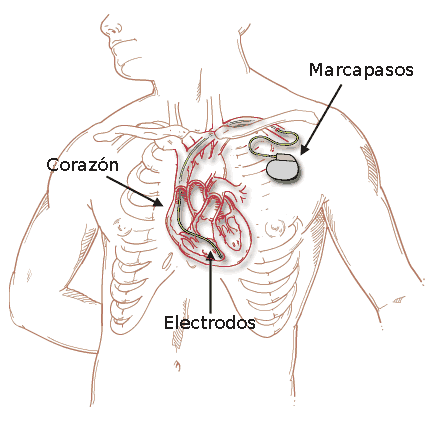
\includegraphics[scale=0.3]{./Introduccion/marcapasos}}
    \subfigure[]{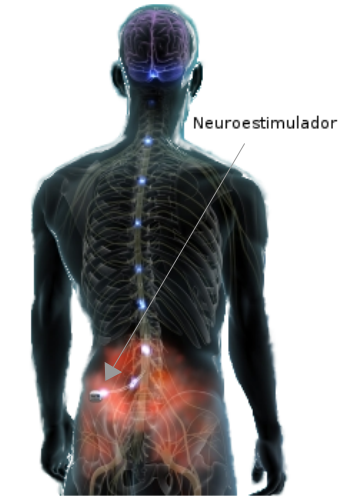
\includegraphics[scale=0.3]{./Introduccion/neuroestimulador}}
    \subfigure[]{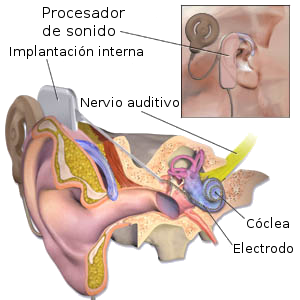
\includegraphics[scale=0.5]{./Introduccion/coclear}}
    \caption{Imágenes de ejemplos de dispositivos médicos implantables. (a) Marcapasos \cite{marcapasos}. (b) Neuroestimulador \cite{neuroestimulador}. (c) Implante coclear \cite{coclear}.}
    \label{fig:fig1.1}
\end{figure}


\section{El sistema de comunicaciones de los dispositivos médicos implantables}\label{sec:enlace}

El uso y tipos de los DMI ha crecido considerablemente desde que en 1958 se implantó el primer marcapasos \cite{brunckhorst}. Desde entonces, los avances en el diseño de los DMI y de sus componentes electrónicos han abierto puertas a funcionalidades más sofisticadas y versátiles. Esta evolución en el diseño de los DMI ha propiciado, a su vez, la posibilidad de configurar las funcionalidades y sus parámetros, pudiendo ser adaptadas a las necesidades de distintos grupos de pacientes.

La configuración de los DMI se realiza a través de un enlace de comunicaciones que pone en contacto al DMI con otro aparato externo. La comunicación del DMI no sólo sirve para programarlo, sino que además suele utilizarse para que el propio dispositivo envíe información recogida por él mismo para procesarla o cualquier otra medida que se lleve a cabo. Debido además a la posición del DMI en el interior del cuerpo humano, lo que hace imposible un contacto físico directo, se ha creado este sistema de comunicaciones en los dispositivos que lo necesiten.

Originalmente, el sistema de comunicaciones de estos dispositivos y otros semejantes ha sido llevada a cabo por un enlace inductivo~\cite{webster,cavuoto}. Sin embargo, este enlace inductivo presenta varias limitaciones: una de ellas es que se debe mantener el dispositivo externo al paciente a muy corta distancia e incluso perfectamente alineado con el DMI; otra limitación es que la capacidad de transferencia de datos es muy baja. Al cabo del tiempo y gracias a los avances arriba mencionados, se ha recurrido al uso de nuevas tecnologías de radiofrecuencia. Estas tecnologías de radiofrecuencia poseen ventajas muy importantes respecto al enlace inductivo: el ancho de banda es mayor (con lo que se puede transmitir y recibir mayor información a una tasa también mayor) y la onda electromagnética transmitida llega más lejos y se atenúa menos, es decir, permite que la comunicación entre el DMI y otro dispositivo sea a mayor distancia. En el capítulo \ref{ch:cap3}, se describen con detalle las tecnologías de radiofrecuencia utilizadas hoy en día para los DMI.

El punto de unión entre los DMI y este Proyecto Fin de Carrera son las antenas que poseen los sistemas de comunicación de estos dispositivos. Estas antenas cumplen una función muy importante, que es la de permitir la comunicación del DMI con otro aparato externo para, como se ha comentado anteriormente, configurar el DMI o recoger información monitorizada del cuerpo o zona del cuerpo donde se ha implantado el dispositivo. El diseño de las antenas debe obedecer varias restricciones impuestas por las características del DMI: deben ser antenas pequeñas, para que puedan ser ubicadas dentro del DMI y que no ocupen mucho espacio; deben ser también antenas eficientes y de bajo consumo, para evitar que el DMI sea reemplazado periódicamente por agotamiento de la batería instalada en el dispositivo y deben ser biocompatibles.

Es por estas razones que hoy en día, el sistema de comunicaciones de los DMI dentro del campo de investigación acutal, sea desarrollado con \textit{antenas microstrip}. Las antenas microstrip fabricadas de manera \textit{embebida}, es decir, fabricadas junto a otros dispositivos, han sido utilizadas por muchas aplicaciones. Destacamos como por ejemplo la aplicación de red de sensores (sensores de movimiento, sensores de humedad, geológicos, etc.) o aplicaciones para la comunicación inalámbrica entre dispositivos, ya sea un teléfono móvil, un GPS, etc~\cite{garg1}. Existen también aplicaciones terapéuticas como es el caso del tratamiento de la hipotermia\footnote{Descenso involuntario de la temperatura corporal por debajo de los 35ºC.} y la hipertermia\footnote{Aumento de la temperatura corporal por encima de los 38ºC; también conocido como \textit{golpe de calor}.} o en uso de catéteres cardíacos~\cite{yang1}. Debido a sus características, que se desarrollan en profundidad en el capítulo~\ref{ch:contexto}, las antenas microstrip son apropiadas para los DMI y su enlace de comunicaciones. Hoy en día son un continuo objeto de estudio por parte de laboratorios de investigación, universidades y empresas ya que son una herramienta muy útil y eficiente para el entorno en el que se desarrolla este Proyecto Fin de Carrera. En el capítulo~\ref{ch:contexto} se proporciona una revisión de trabajos previos de antenas microstrip para DMI.


\section{Objetivos del Proyecto Fin de Carrera}\label{sec:objetivos}

Este Proyecto Fin de Carrera se enmarca dentro del campo de las antenas microstrip para DMI. El \textbf{objetivo global} de este PFC es:

\begin{itemize}

    \item Estudiar, analizar y caracterizar una antena microstrip propuesta en un artículo de la literatura revisada para los sistemas de comunicaciones de los DMI \cite{soont}.
\end{itemize}

\clearpage

\begin{flushleft}
    Otros \textbf{objetivos parciales} recogidos en el proyecto son:
\end{flushleft}

\begin{itemize}
    \item Estudiar la tecnología microstrip, su funcionalidad, ventajas, desventajas y aplicaciones;
    \item Analizar los distintos métodos numéricos de análisis de antenas existentes y en concreto, para las antenas microstrip;
    \item Conocer las propiedades electromagnéticas de los tejidos humanos;
    \item Realizar una revisión bibliográfica de las antenas microstrip, en particular, artículos de investigación actual de antenas microstirp para DMI;
\end{itemize}


\section{Estructura del Proyecto Fin de Carrera}\label{sec:contenidos}

El recorrido por este Proyecto Fin de Carrera está compuesto por cinco capítulos principales:

\begin{itemize}
    \item En el \textbf{Capítulo \ref{ch:contexto} \textit{Contexto tecnológico de las antenas microstrip}}, se presentan las características principales de las antenas microstrip, en especial, las antenas rectangulares. Podemos ver los distintos tipos de análisis teóricos que existen para las mismas, además de sus modos de alimentación. Algunas aplicaciones para DMI se describen al final del capítulo.
    \item En el \textbf{Capítulo \ref{ch:cap3} \textit{Propiedades y modelos electromagnéticos del cuerpo humano y bandas de frecuencia}}, se analizan las distintas propiedades de los tejidos humanos o animales, los modelos de estudio para el cuerpo humano y por último las bandas de frecuencias utilizadas para los DMI.
    \item En el \textbf{Capítulo \ref{ch:metodos} \textit{Metodología}}, se introducen las distintas herramientas que han sido utilizadas en este Proyecto Fin de Carrera.
    \item En el \textbf{Capítulo \ref{ch:simulaciones} \textit{Simulaciones de antenas microstrip en forma de serpentina}}, se entra de lleno en la parte de la simulación de la antena propuesta y distintas variantes a la misma. Estudiamos los distintos parámetros de la antena como son el parámetro $S_{11}$, los campos eléctricos y el diagrama de radiación.
    \item En el \textbf{Capítulo \ref{conclusiones} \textit{Conclusiones y líneas futuras}}, se describen los objetivos conseguidos en este Proyecto Fin de Carrera y las conclusiones finales. Las líneas futuras que se han ido mencionando a lo largo de este texto, quedan recogidas aquí.
    \item En el \textbf{Apéndice I. Presupuesto} se muestra un cálculo aproximado de las horas trabajadas en este Proyecto Fin de Carrera.
    \item En el \textbf{Apéndice II. Artículo wiki} se menciona el aporte extra que acompaña a esta memoria, un artículo wiki alojado en la web del departamento de TSC de la URJC.
\end{itemize}

    \newpage \thispagestyle{empty} \cleardoublepage

%===============================================================
%CONTEXTO TECNOLÓGICO
%===============================================================
    \chapter{\textbf{Contexto tecnológico de las antenas microstrip}}\label{ch:contexto}

En este capítulo veremos las características principales de las antenas microstrip. No entraremos en detalle con estudio analítico ya que no es objeto de este proyecto. Desde la sección~\ref{sec:conceptos} a la sección~\ref{sec:alimentacion} veremos los conceptos generales de análisis de las antenas microstrip. Prosiguiendo esta línea, en la sección~\ref{sec:aplicaciones} abordaremos las distintas aplicaciones de estas antenas y en la sección~\ref{sec:aplicacionesdmi} proporcionaremos una revisión bibliográfica de antenas microstrip para DMI.


\section{Conceptos básicos}\label{sec:conceptos}

Los elementos radiantes con característica microstrip fueron descritos originariamente por Deschamps en 1953~\cite{deschamps}. No fue hasta veinte años después, cuando se fabricaron las primeras antenas microstrip. El desarrollo durante la década de los setenta de mejores substratos y modelos teóricos más fiables, propició un crecimiento muy grande en el desarrollo de dichas antenas. A partir de la creación de la primera antena microstrip práctica por Howell y Munson~\cite{howell,munson}, se hicieron investigaciones exhaustivas sobre este campo y el uso de configuración en arrays de las mismas antenas~\cite{bahl,james1,james2}. Fueron muchas las ventajas descritas en ese momento respecto a otra clase de antenas, como por ejemplo su bajo peso y volumen, su reducido coste y además la facilidad de fabricarlas y depués configurarlas. Esto propició que se desarrollara en masa este tipo de antenas para diversos campos de estudio y aplicaciones, las cuales podremos ver en este capítulo.

Una \textbf{antena microstrip} consiste en un \textbf{parche} o \textbf{estructura radiante} formado de material conductor, que suele ser cobre, oro, aluminio, etc., colocado encima de una capa de \textbf{substrato dieléctrico} con una cierta permitividad relativa $\epsilon_{r}$ y por debajo de estas dos capas, \textbf{un plano de masa} de material conductor. Dicha antena puede ser alimentada de muchas maneras, a través de líneas microstrip, coaxiales u otros elementos radiantes, tal y como veremos en una próxima sección. Los materiales dieléctricos del substrato suelen tener una $\epsilon_{r}$ menor de 10 para no perder eficiencia en la antena~\cite{garg}.

\begin{figure}[!htb]
    \centering
    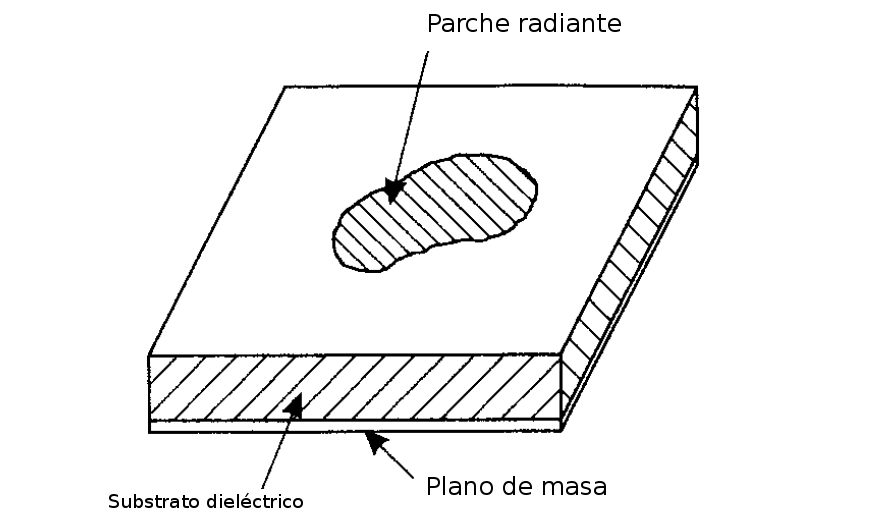
\includegraphics[scale=0.25]{./ContextoTecnologico/antena_parche}
    \caption{Dibujo de un esquema sencillo de una antena de parche o antena microstrip.}
    \label{fig:fig2.1}
\end{figure}

El conductor del parche como hemos dicho suele ser de un metal conductor con diversas formas geométricas posibles dependiendo de la aplicación y/o polarización requerida, aunque las más habituales suelen ser formas regulares (cuadrado, rectángulo, círculo, etc.). Para conseguir los campos que van hacia el exterior de la antena y ayudan a que aparezca la radiación, la constante dieléctrica  $\epsilon_{r}$ del substrato de la antena idealmente debe tener un valor bajo. Debido a esto, se han desarrollado varios tipos de substratos con óptimas propiedades en dicha variable, además de conseguir valores mínimos en pérdidas tangenciales\footnote{Término matemático que indica si es mayor la corriente de conducción o la corriente de desplazamiento cuando un campo electromagnético se propaga a través de cierto material. Proporciona las pérdidas de energía del dieléctrico.} del mismo dieléctrico. Estos materiales suelen ser moldeables, por lo que son apropiados para este tipo de antenas. Con respecto a los tipos de materiales utilizados para el substrato de una antena, éstos pueden ser de muchos tipos, entre los que destacamos: panal de miel (\textit{honeycomb}), cuarzo, grasas industriales, Duroid, ARLON1000, Macor, etc.

\clearpage

Muchas son las ventajas de las antenas de parche o microstrip, entre las que podemos enumerar~\cite{garg}:
\begin{itemize}
    \item Cubren aplicaciones que trabajan en un rango de frecuencias de 100 MHz a 100 GHz;
    \item Bajo peso, bajo volumen y configuraciones simples que pueden ser rediseñadas;
    \item Con una única alimentación, es posible obtener polarizaciones lineales y circulares;
    \item Su fabricación es muy simple y de bajo coste;
    \item Es posible crear antenas que trabajan en bandas duales;
    \item Pueden ser integradas perfectamente junto a circuitos de microondas;
    \item Algunas líneas y redes de alimentación pueden ser fabricadas simultáneamente junto a la estructura de la antena.
\end{itemize}

\begin{flushleft}
    Algunas de las limitaciones de las antenas microstrip son:
\end{flushleft}
\begin{itemize}
    \item Ancho de banda estrecho;
    \item Baja ganancia, alrededor de 6 dB;
    \item Es difícil conseguir una polarización pura;
    \item Un uso de un substrato de alta constante dieléctrica lleva asociado una pobre eficiencia y un reducido ancho de banda.
    \item Existe un constante compromiso entre muchas variables de la antena a fabricar: constante dieléctrica, ancho y largo, ancho del substrato, alimentación, etc.
\end{itemize}

Estas limitaciones pueden ser subsanadas si se aplican por ejemplo técnicas avanzadas que se alejan de nuestro estudio, como el uso de configuración array si se tiene una antena con muy baja ganancia~\cite{garg9}.


\section{Mecanismo de radiación}\label{sec:mecanismo}

La radiación de las antenas microstrip puede ser descrita en términos de distribución de campos alrededor de la superficie del parche conductor o de corrientes en la antena. Para calcular dicha distribución de campos de manera analítica hacen falta cálculos y métodos muy complejos~\cite{balanis14}, cosa que se aleja de nuestro estudio.

Para explicar el mecanismo de radiación, vamos a analizar de manera cualitativa una estructura muy sencilla de antena microstrip a la que se ha conectado una fuente de microondas. Como vemos en \textit{fig. \ref{fig:fig2.2}}, cuando el parche conductor recoge la energía procedente de la fuente, se establecen cargas entre la parte de arriba y la de abajo del propio parche conductor. Simultáneamente en el plano de masa se genera otra distrubución de cargas.

\begin{figure}[!htb]
    \centering
    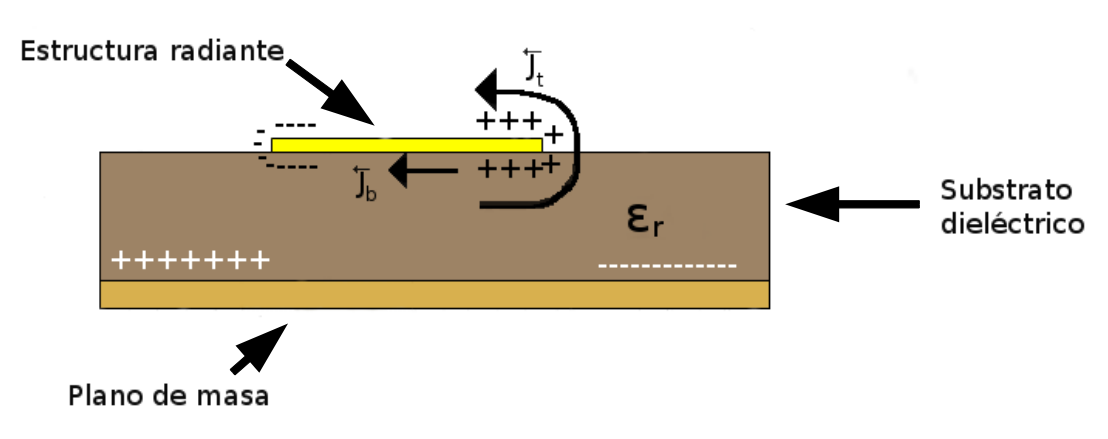
\includegraphics[scale=0.4]{./ContextoTecnologico/cargas_parche_4}
    \caption{Dibujo de las cargas de corriente que aparecen en la antena microstrip cuando se alimenta.}
    \label{fig:fig2.2}
\end{figure}

Las fuerzas resultantes repulsivas que aparecen entre las cargas de la parte de abajo del parche y la parte de la superficie, provocan un movimiento que desplaza a las cargas de abajo hacia arriba. Este movimiento crea dos \textbf{densidades de corriente} $\vec{J}$ tanto en la superficie como en la parte de abajo del parche. Es así como la fuerza atractiva entre las cargas predomina y debajo del parche es donde se acumula la mayor concentración de carga. Esto provoca pequeños flujos de corriente en los límites del parche hacia la superficie, siendo responsables de un débil campo magnético tangencial. Estas cargas además son el origen de los campos radiantes y de la radiación deseada, la cual puede ser aumentada utilizando un grosor mayor de substrato junto a un valor de $\epsilon_{r}$ suficientemente bajo para lograrlo. Sin embargo, la radiación de una estructura microstrip, tanto una antena como una línea, puede ser reducida si se utiliza un substrato dieléctrico con una alta constante relativa $\epsilon_r$ o en cambio, con una capa de substrato muy delgada. Por ello, las capas de substrato utilizadas deben ser anchas para permitir una radiación efectiva sin empeorar la eficiencia de dicha estructura. Como se puede deducir, existe un compromiso de diseño entre el ancho de la capa de substrato y el índice dieléctrico del material de la misma.


\section{Tipos de onda}\label{sec:ondas}

Tras ver cómo es posible el mecanismo de radiación, veremos qué tipos de ondas se forman en este tipo de antenas. Existen cuatro tipos de onda en una línea microstrip: las ondas espaciales, las ondas superficiales, las ondas de fuga y las ondas de guía \cite{balanis2}\cite{bhartia}.

\subsection{Ondas espaciales}\label{subsec:ondas-espaciales}

Las ondas espaciales son las ondas enviadas al espacio libre y sufren atenuación a medida que se alejan de su fuente. En el diseño de antenas, son las ondas más importantes a tener en cuenta, porque son las ondas radiadas. En el caso en el que se diseñan líneas de transmisión o circuitos, estas ondas son la causa de pérdidas y mal funcionamiento en la aplicación buscada y por tanto, deben eliminarse.

\subsection{Ondas superficiales}\label{subsec:ondas-superficiales}

Las ondas superficiales son las ondas que en su mayoría están recluídas dentro del substrato dieléctrico. No son ondas uniformes, ya que cuando viajan por esta capa son reflejadas una y otra vez por el plano de tierra y por la cara anterior del parche conductor. Las ondas superficiales permanecen viajando y perdiendo amplitud, tomando parte de la señal que se quiere enviar y aumentando las pérdidas en la transmisión. Esto provoca también un acoplamiento incorrecto del circuito de la antena.

\subsection{Ondas de fuga}\label{subsec:ondas-de-fuga}

Las ondas de fuga se forman cuando las ondas que viajan por el substrato dieléctrico llegan al lateral del substrato y se dividen entre las que se \textit{fugan} al espacio libre y las que se reflejan de nuevo.

\subsection{Ondas guiadas}\label{subsec:ondas-guiadas}

Las ondas guiadas aparecen en las antenas que tienen cubierto su parte superior casi por completo de material conductor: las ondas viajan por el substrato dieléctrico y al estar rebotando todo el rato por las partes metálicas, quedan recluídas dentro de la antena como si fuera un circuito. En el diseño de antenas esto se debe evitar.


\section{Alimentación}\label{sec:alimentacion}

Otro de los aspectos importantes del diseño de antenas, ya sean microstrip o de otro tipo, es el modelo de alimentación que tienen. Una antena con un mal diseño de alimentación puede llevar a un mal funcionamiento de la misma. A través de un correcto acoplamiento de impedancias, se puede conseguir que la antena radie en la banda de frecuencias deseada. Estudiaremos en nuestro caso tres métodos distintos: \textit{alimentación directa}, \textit{alimentación por proximidad} y \textit{alimentación por apertura} \cite{garg,bhartia}.

\subsection{Alimentación directa}\label{subsec:alimentacion-directa}

Este método de alimentación necesita que tanto la estructura de alimentación como el parche radiante estén unidos o en contacto. La principal desventaja de este método es que a la hora de diseñar, existe un compromiso muy estrecho entre las características de radiación de la antena y las características propias del modelo de alimentación. Ambas no se pueden optimizar por separado al estar unidas, ya que ambos se encuentran en una misma capa de substrato en la mayoría de diseños. Dentro de esta misma categoría de alimentación nos encontramos con dos tipos diferentes: la \textit{alimentación por microstrip} y la \textit{alimentación por coaxial}.

\subsubsection{Alimentación por microstrip}

La alimentación por microstrip o por tira conductora, consiste simplemente en alimentar al parche radiante por medio de una línea o tira microstrip con una impedancia diseñada con anterioridad. Este modelo es muy fácil de diseñar y fabricar pero conlleva no obstante una pérdida notoria en ancho de banda, acoplamiento y eficiencia. Las dos formas más comunes de alimentar una antena por medio de una tira microstrip son conectando la línea microstrip \textit{directamente en un borde de la antena} o alimentando la linea microstrip \textit{a través de inserciones en la antena}. El acoplamiento de impedancia dependerá de la posición de la línea con el parche radiante en el primer caso y en el segundo dependerá de la longitud de la inserción. Este método se aprecia en la \textit{fig. \ref{fig:fig2.3}}

\begin{figure}[!htb]
    \centering
    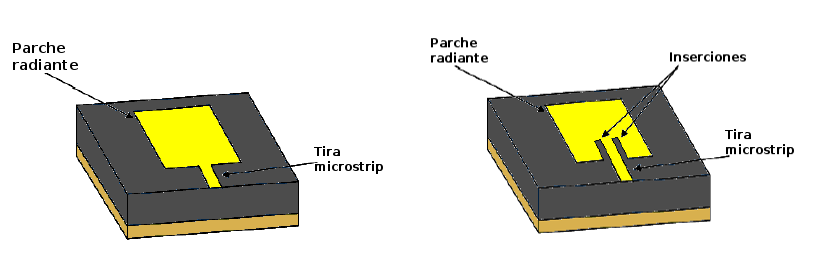
\includegraphics[scale=0.55]{./ContextoTecnologico/microstrip_feed}
    \caption{Ejemplo de antenas con alimentación microstrip. Izquierda: conexión directa al borde de la antena. Derecha: conexión con inserciones.}
    \label{fig:fig2.3}
\end{figure}

\subsubsection{Alimentación por coaxial}

La alimentación por coaxial se basa en colocar el pin del cable coaxial directamente al parche radiante y la parte negativa del pin a la capa de tierra o masa de la antena. Tendremos una impedancia u otra dependiendo de cómo coloquemos el coaxial con respecto a la antena y al parche radiante. Este método es uno de los más utilizados, pero su construcción es difícil ya que el pin del cable debe atravesar el substrato y a la vez estar soldado a la propia antena para su correcto funcionamiento. En la \textit{fig. \ref{fig:fig2.4}} podemos ver una estructura ejemplo.

\begin{figure}[!htb]
    \centering
    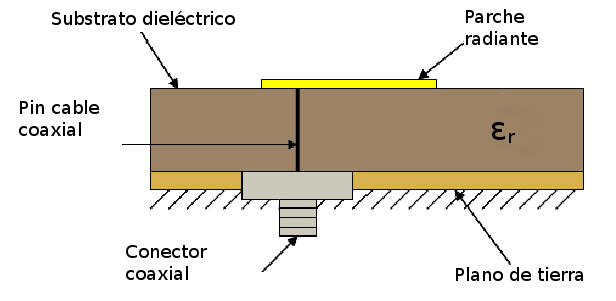
\includegraphics[scale=0.55]{./ContextoTecnologico/coaxial}
    \caption{Estructura ejemplo de una conexión para la alimentación por medio de un cable coaxial.}
    \label{fig:fig2.4}
\end{figure}

\subsection{Alimentación por proximidad}\label{subsec:alimentacion-por-proximidad}

La alimentación por proximidad ocurre en este caso por medio de un acoplamiento electromagnético. Consiste en separar la estructura del parche radiante de la estructura de alimentación para optimizar por separdo cada parte. Lo más normal es colocar el parche radiante en un substrato con una constante de permitividad relativa baja; debajo de éste la tira microstrip con un substrato con permitividad relativa alta y debajo de todas estas capas, el plano de masa o tierra. La \textit{fig. \ref{fig:fig2.5}} representa un ejemplo de la estrucutra de alimentación por proximidad.

\begin{figure}[!htb]
    \centering
    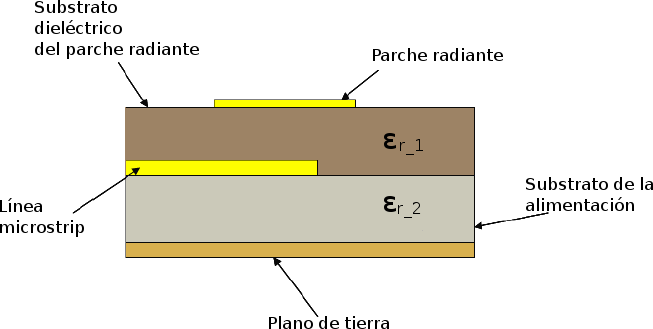
\includegraphics[scale=0.45]{./ContextoTecnologico/proximidad_2}
    \caption{Estructura ejemplo de la alimentación por proximidad.}
    \label{fig:fig2.5}
\end{figure}

\subsection{Alimentación por apertura}\label{subsec:alimentacion-por-apertura}

El método de alimentación por apertura consiste en diseñar una antena con estas capas: un parche radiante sobre un substrato dieléctrico, los cuales están encima de un plano de tierra compartido por otro substrato dieléctrico que tiene por debajo una línea microstrip de alimentación. Tiene muchas similitudes con el método de alimentación por proximidad, pero en este caso, el plano de tierra, que es común, tiene una apertura o agujero cuya posición y dimensiones participan directamente en el valor de la impendancia y por lo tanto, en el acoplamiento de la antena. Una ventaja a destacar con respecto a la alimentación por proximidad es que al estar más separadas las estructuras radiante y la de alimentación, la radiación de esta última no influye en la dirección de propagación de la onda resultante; evita además la aparición de interferencias y polarizaciones. Una estructura ejemplo se puede apreciar en la \textit{fig. \ref{fig:fig2.6}}.

\begin{figure}[!htb]
    \centering
    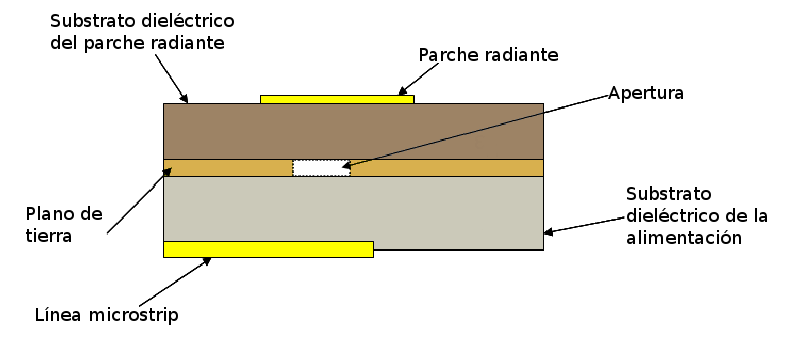
\includegraphics[scale=0.45]{./ContextoTecnologico/apertura}
    \caption{Estructura ejemplo de la alimentación por apertura.}
    \label{fig:fig2.6}
\end{figure}


\section{Antenas microstrip rectangulares}\label{rectangular}

Las antenas tipo parche rectangulares son las más utilizadas debido a su facilidad de diseño y de implementación en diversos dispositivos. Además de conseguir fácilemente la polarización, su estudio y análisis son bastante simples.

La configuración más sencilla posible de una antena microstrip es una antena en forma rectangular, cuyo parche conductor tiene dimensiones \textit{L} x \textit{W} (largo x ancho) situado encima de una capa de substrato con constante dieléctrica $\epsilon_r$ y anchura \textit{h}, la cual descansa sobre una última capa de plano de masa. Podemos ver esta estructura de antena en la \textit{fig. \ref{fig:fig2.7}}.

\begin{figure}[!htb]
    \centering
    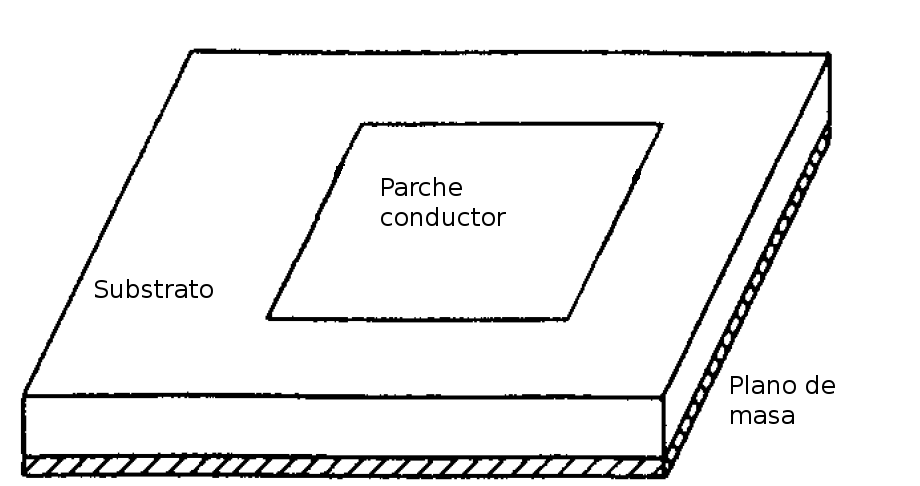
\includegraphics[scale=0.25]{./ContextoTecnologico/antena_rectangular}
    \caption{Dibujo ejemplo de una antena microstrip rectangular.}
    \label{fig:fig2.7}
\end{figure}

\subsection{Consideraciones de diseño}\label{subsec:consideraciones-de-diseno}

El objetivo principal del diseño es conseguir por ejemplo, un resultado específico a una frecuencia estipulada. En el diseño de una antena microstrip, el primer paso es la elección del tipo de substrato con una adecuada constante dieléctrica y el grosor de su capa $h$. Una capa ancha incrementa la potencia radiada, reduce las pérdidas por conducción e incrementa el ancho de banda. Sin embargo, esto aumenta el peso, las pérdidas del dieléctrico en sí y las pérdidas por ondas superficiales, además de las pérdidas por conectores. Es posible que una antena microstrip rectangular deje de emitir en su frecuencia de resonancia debido al grosor de esta capa y a la reactancia surgida en la alimentación~\cite{pozar}.\\

El valor de la constante dieléctrica $\epsilon_{r}$ es fundamental también para el diseño ya que un valor pequeño de éste incrementa el campo exterior radiado, la potencia radiada y por tanto la eficiencia de la antena; en cambio, un valor grande provoca todo lo contrario. Estudios realizados en \cite{garg4}, aseguran que el objetivo en el diseño es encontrar un substrato con índices de $\epsilon_{r}$ menores a 2,5.

Existe además un compromiso entre el grosor de la capa de substrato y la constante dieléctrica del mismo, ya que aumentar el ancho de la capa tiene el mismo efecto que disminuir $\epsilon_{r}$. Los elementos más utilizados para el substrato de antenas tipo parche son:

\begin{itemize}
    \item Honeycomb, con $\epsilon_{r}$ = 1.07;
    \item Duroid, con $\epsilon_{r}$ = 2.32;
    \item Cuarzo, con $\epsilon_{r}$ = 3.8;
    \item Arlon, con $\epsilon_{r}$ variable;
    \item y Alumina, con $\epsilon_{r}$ = 10.
\end{itemize}

Otras consideraciones parten del ancho $W$ y largo $L$ de la estructura de la antena. En~\cite{garg4} se sugiere que las dimensiones deben cumplir esta relación: $1 < W/L <2$. El ancho por ejemplo, afecta a la resistencia de entrada y al ancho de banda. El largo por otro lado, determina la frecuencia de resonancia y es crítico en el diseño debido a como hemos mencionado antes, el estrecho ancho de banda que proporcionan estas antenas. Puede incluso incrementar la potencia radiada, el ancho de banda y la eficiencia de radiación. No todos los campos quedan confinados en la región de $L$ x $W$ como se ha podido ver en en la sección~\ref{sec:ondas}; esto es lo que provoca realmente que la antena radie ondas electromagnéticas~\cite{garg4}.

\subsection{Métodos para el estudio de antenas microstrip rectangulares}\label{subsec:teoria}

En esta sección veremos dos modelos para el estudio de las antenas microstrip rectangulares los cuales facilitan mucho el estudio teórico y la asimilación de conceptos: el método de línea de transmisión y el método de cavidad.

\subsubsection{Método de línea de transmisión}

Las antenas microstrip tienen una estructura que deriva directamente de una línea de transmisión microstrip. En este modelo, la antena es modelada como una línea de transmisión de longitud L, una impedancia característica $Z_{0}$ y una constante de propagación que se deriva de la ecuación $\gamma = \alpha + j\beta$, donde $\alpha$ es la constante de atenuación de la línea y $\beta$ es la constante de fase de la misma. Los campos electromagnéticos varían a lo largo del parche, que suelen ser de media onda y la radiación se produce en este caso debido a los terminales que están en circuito abierto.\\

\begin{figure}[!htb]
    \centering
    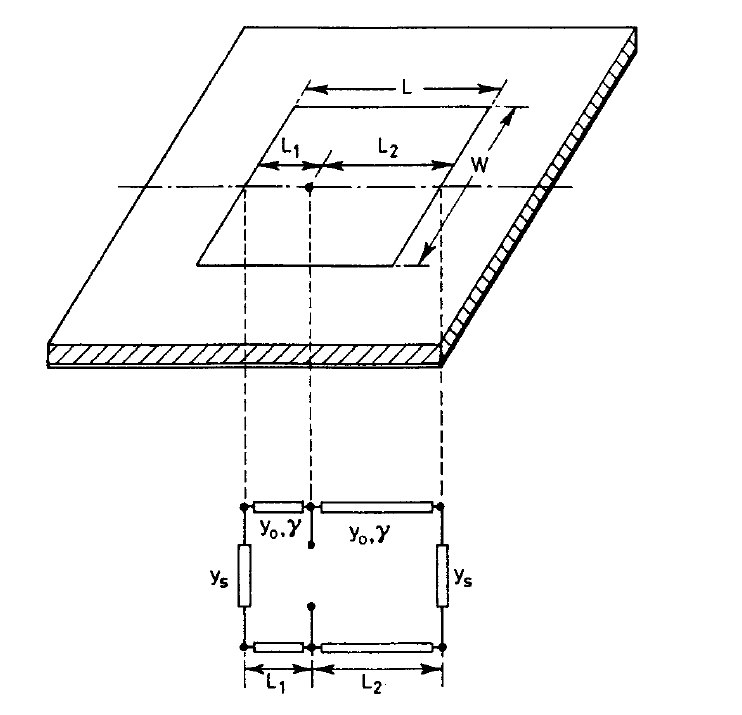
\includegraphics[scale=0.25]{./ContextoTecnologico/ejemplo_linea}
    \caption{Ejemplo de análisis de una estructura microstrip como línea de transmisión.}
    \label{fig:fig2.8}
\end{figure}

Existen muchos estudios sobre este método y la manera de desarrollar las ecuaciones del mismo para encontrar los parámetros de la línea, es decir cómo obtener la impendacia de entrada $Z_{in}$, la constante de fase $\beta$ y la auto-admitancia $Y_{S}$ (encontrada al final de la línea en circuito abierto y que recoge el efecto de la radiación de la línea)~\cite{munson,derneryd,pues}.

\subsubsection{Método de cavidad}

Otro punto de vista por el que podemos ver las antenas microstrip, es el de cavidad resonante. Las antenas microstrip son resonantes de banda estrecha, de ahí este nombre para este método de análisis.

En este modelo, el interior de la estructura de la antena es modelado como una cavidad rodeada de paredes eléctricas tanto en la parte inferior como superior y de una pared magnética a los lados. Existen unas bases para este modelo, asumiendo siempre que $h << \lambda_{0}$, es decir, que la altura de la capa de substrato sea mínima frente a la longitud de onda de resonancia \cite{richards}:

\begin{itemize}
    \item Los campos en el interior no varían con $z$, porque el substrato es muy delgado;
    \item El campo eléctrico viaja sólo en dirección $z$ y el campo magnético confinado entre el parche conductor y el plano de masa sólo tiene componentes $H_{x}$ y $H_{y}$;
    \item La corriente eléctrica en la dirección normal del parche conductor es cero, lo que implica que la componente tangencial del campo magnético a lo largo de los lados parche es cero y de esta forma la pared magnética está situada allí.
\end{itemize}

\begin{figure}[!htb]
    \centering
    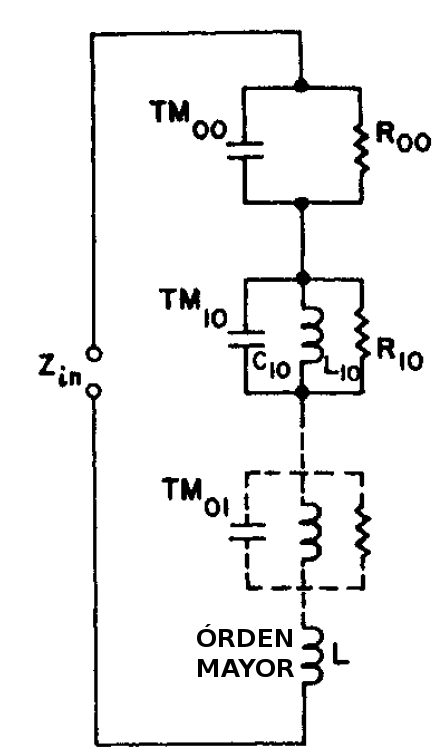
\includegraphics[scale=0.25]{./ContextoTecnologico/ejemplo_cavidad}
    \caption{Circuitos ejemplo tras el análisis del modelo de cavidad.}
    \label{fig:fig2.9}
\end{figure}

La distribución de campo está divida en dos regiones, los campos en el interior de la estructura y los campos que están en el exterior. Los campos externos son los que salen hacia afuera de la cavidad y determinan las características de radiación del parche. Así mismo, los campos internos de la cavidad nos proporcionan información acerca de la impendancia de entrada de la antena y las corrientes responsables de dicha radiación. Estos campos se determinan a través de las cuatro ecuaciones fundamentales del electromagnetismo descritas por Maxwell y su desarrollo para obtener la ecuación de onda.

Todo ese desarrollo determina la ecuación para obtener el campo eléctrico en la dirección de propagación $E_{z}$, la impedancia de entrada y fundamentalmente, los modos de trabajo de la cavidad. Los modos más básicos pueden ser representados mediante sencillos circuitos RLC como vemos en la \textit{fig \ref{fig:fig2.9}} \cite{garg4}.


\section{Aplicaciones}\label{sec:aplicaciones}

Las antenas microstrip o de tipo parche fueron inicialmente desarrolladas y utilizadas en aplicaciones militares, tales como diseño de misiles y/o cohetes, en la aviación y en la mejora de los sistemas de satélites \cite{garg1}. En la actualidad estas antenas han visto aumentado su uso en muchas otras áreas, debido especialmente al reducido coste de su fabricación. Es más, en muchas aplicaciones, las antenas convencionales pueden ser sustituidas por antenas de parche o microstrip.

\begin{flushleft}
    Algunas aplicaciones que han podido desarrollar antenas microstrip son:
\end{flushleft}

\begin{itemize}
    \item Comunicaciones vía satélite tipo broadcast (DBS);
    \item Radares Doppler y otros;
    \item Misiles y telemetría espacial;
    \item Alimentación en antenas con estructuras complejas;
    \item Comunicaciones móviles;
    \item Antenas integradas en dispositivos de comunicaciones;
    \item Elementos radiantes biomedicinales;
    \item Alarmas de intrusión.
\end{itemize}

Veremos a continuación con detalle algunas de estas interesantes aplicaciones en los campos de la comunicación terrestre y satélite, además de implementaciones para uso médico.

\subsection{Aplicaciones en comunicaciones móviles y vía satélite}\label{subsec:aplicaciones-en-comunicaciones-moviles-y-via-satelite}

Las comunicaciones móviles requieren dispositivos ligeros, pequeños y en consecuencia, antenas de bajo coste y poco volumen para integrar muchas otras herramientas \cite{james2}\cite{huang}. Las antenas microstrip cumplen este último propósito y para ello, se han desarrollado varios modelos de las mismas para distintas aplicaciones y sistemas de comunicaciones móviles. Muchas de estas antenas que trabajan en rangos que van de MHz a GHz han sido integradas en radares, barcos, aviones, teléfonos celulares e incluso en sistemas automovilísticos para evitar colisiones.

Las antenas aplicadas a las comunicaciones vía satélite utilizan en algunas aplicaciones la polarización circular. Para ello, se diseñan antenas microstrip con forma de parche circular con uno o más puntos de alimentación en ella \cite{garg8}. Pero existen algunos problemas en el desarrollo de estas antenas, como por ejemplo el límite de potencia que puede dar el satélite o el tamaño máximo de la antena o incluso, la ganancia de la misma para obtener una fiable comunicación entre el satélite y la Tierra. Es en este caso cuando se han diseñando arrays de antenas microstrip, consiguiendo mucha más directividad, ganancia y bajo coste en la implementación. Muchas de ellas son construidas bajo el criterio de uso de unos modos de onda concretos TM.

Otra interesante aplicación vía satélite que empezó siendo un proyecto militar hace 30 años y ahora es una realidad cotidiana es el \textbf{GPS} o \textbf{Sistema de Posicionamiento Global} \cite{garg1}. Actualmente, este sistema es utilizado por millones de dispositivos o vehículos en cualquier parte del mundo para determinar su posición y altura de manera exacta. El GPS consiste en 24 satélites que orbitan alrededor de la Tierra a unos 20.000 kms. de distancia. Para obtener este servicio, se necesitan antenas de polarización circular omnidireccionales y de baja ganancia. Las antenas microstrip son adecuadas para este trabajo, minimizando el tamaño de la antena, el peso y el coste de la misma en la banda L de frecuencias (1573-1577 MHz), que es la que utiliza el GPS.

Las aplicaciones correspondientes a las comunicaciones móviles terrestres es el campo donde el desarrollo e integración de las antenas microstrip está extendido globalmente \cite{garg1}. Las antenas que normalmente llevan los dispositivos celulares suelen ser de pequeño tamaño y por supuesto compactas. Un problema existente en este tipo de comunicaciones es la baja eficiencia y ganancia de las antenas. El problema puede ser resuelto modificando el diseño de las antenas mediante substratos con un dieléctrico con $\epsilon_r$ más alto o incluso colocando arrays de antenas.

\subsection{Aplicaciones en medicina}\label{subsec:aplicaciones-en-medicina}

Las ondas de microondas han sido estudiadas profundamente en el campo de la medicina como una manera efectiva de combatir la hipotermia y tratar tumores malignos. Un elemento radiante que se utilice para estos propósitos y que se aplique directamente en la superficie a tratar debe ser ligero, flexible y fácil de manejar. Este elemento por ejemplo puede ser un parche con estructura radiante.

Algunos diseños de estructuras microstrip utilizadas son los dipolos impresos o los anillos anulares en la banda S para tratar la hipotermia \cite{sterzer}. Hay otros casos de discos circulares microstrip en la banda L para el mismo cometido \cite{deleo}. En otro caso, para medir la temperatura del cuerpo humano, se ha utlizado dos líneas microstrip con separación variable y ajustable~\cite{kobay1}. Un uso de esta aplicación, la cual va encaminada a nuestro estudio, se puede ver en la \textit{fig. \ref{fig:fig2.10}}.

\begin{figure}[!htb]
    \centering
    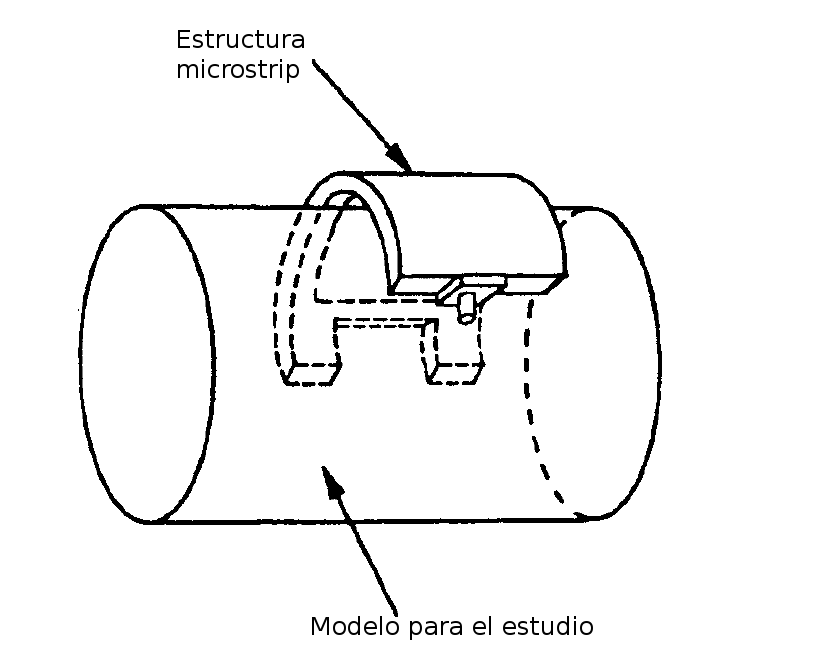
\includegraphics[scale=0.2]{./ContextoTecnologico/antena_medicina}
    \caption{Ejemplo de aplicación de una estructura microstrip flexible para uso medicinal trabajando a una frecuencia de 430 MHz. \cite{kobay2}}
    \label{fig:fig2.10}
\end{figure}


\section{Antenas microstrip en dispositivos médicos implantables}\label{sec:aplicacionesdmi}

En la anterior sección, se han mencionado algunas de las aplicaciones más destacables de las antenas microstrip, con especial mención de la última parte para uso médico. A lo largo de la actual sección, vamos a citar algunos ejemplos de diseños de antenas microstrip para sistemas de comunición de los DMI.

En la literatura acerca de diseños de antenas microstrip para DMI podemos encontrar múltiples estudios. En \textit{Antennas for Over-Body-Surface Communication at 2.45 GHz} de Conway et al. \cite{conway} tenemos un ejemplo de diseño de antenas microstrip para la comunicación de DMI colocados a lo largo de la superficie del cuerpo. En este caso los autores intentan máximizar el parámetro $S_{21}$ entre dos o más dispositivos para conseguir una enlace de comunicaciones fiable. Las antenas microstrip emiten a la frecuencia 2.45 GHz, centrados en la banda ISM (\textit{Industrial, Scientific and Medical band}), frecuencia en la que los autores estudian la posibilidad de tener ondas que se propagan a lo largo de la superficie del cuerpo. Para ello, en el artículo se proponen cinco tipos de antenas microstrip y se realiza un estudio paramétrico de cada una de ellas para la banda mencionada.

\begin{figure}[!htb]
    \centering
    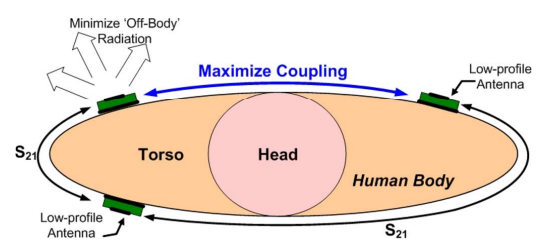
\includegraphics[scale=0.4]{./ContextoTecnologico/articulos/conway1}
    \caption{Esquema del estudio de antenas microstrip sobre la superficie del cuerpo para su comunicación obtenido del artículo \cite{conway}.}
    \label{fig:fig2.11}
\end{figure}

Tras algunas simulaciones y pruebas reales en laboratorio con las antenas, los autores concluyen que el tipo de antena HMMPA (\textit{Higher Mode Microstrip Patch Antenna}), es decir, antenas tipo parche con un alto modo de propagación de onda, son las más adecuadas para este tipo de investigación, ya que obtienen unos resultados parecidos a antenas tipo monopolo\footnote{Antenas formadas por un solo brazo rectilíneo en posición vertical.}. El parámetro $S_{21}$ que obtienen es eficiente y no hay tanta pérdida de potencia como en otras antenas.\\

Otro artículo interesante es el titulado \textit{Dual-band microstrip patch antenna based on short-circuited ring and spiral resonators for implantable medical devices}~\cite{requena} escrito por C.J. Sánchez-Fernández et al., en el cual se propone un diseño innovador para el parche radiante de las antenas microstrip. El parche está formado por una espiral y un anillo cortocircuitado, con lo que proporciona a la antena la característica de ser dual, es decir, que pueda emitir en dos bandas de frecuencias. Este esquema lo podemos ver en la \textit{fig. \ref{fig:fig2.12}}. En este caso, la antena es capaz de emitir tanto en la banda MICS (\textit{Medical Implant Communication Service band}) (402-405 MHz) como en la banda ISM (\textit{Industrial, Scientific and Medical band}) (2.4-2.48 GHz). El diseño de la antena está compuesto de dos capas de substrato dieléctrico: un superestrato para proteger al parche y un substrato para conseguir el efecto de radiación.

\begin{figure}[!htb]
    \centering
    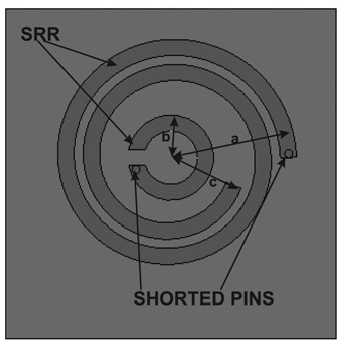
\includegraphics[scale=0.4]{./ContextoTecnologico/articulos/requena1}
    \caption{Diseño del parche radiante la antena microstrip dual descrita en \cite{requena}.}
    \label{fig:fig2.12}
\end{figure}

La espiral del parche hace que la antena radie en la banda MICS y el anillo cortocircuitado en la banda ISM. Los autores realizan diversos experimentos en simulación con la antena sobre distintos medios, como el entorno muscular, el entorno de tres tejidos (piel, músculo y grasa) y en un modelo de cuerpo humano completo. Una de las ventajas que posee esta antena es su reducido tamaño respecto a otras antenas microstrip para DMI. La alimentación de la antena, que es a partir del método de proximidad, consigue un nivel de libertad mayor respecto a otras antenas, sujetas a la alimentación por medio de conexiones coaxiales u otro tipo. Los autores concluyen argumentando que la antena cumple su misión presentando las pruebas realizadas en laboratorio del parámetro $S_{11}$ medidas en un gel con características parecidas al tejido humano de la piel.\\

Un nuevo diseño de antena microstrip lo podemos encontrar en el artículo llamado \textit{Implanted Antennas Inside a Human Body: Simulations, Designs, and Characterizations} \cite{kim}, escrito por J. Kim y Y. Rahmat-Samii. En el artículo, a parte de mencionar los distintos tipos de simulaciones y caracterizaciones que se pueden realizar de un estudio electromagnético para DMI, se propone un diseño de parche radiante en forma de serpentina. Es una antena de bajo coste, pequeña y eficiente que emite en la banda MICS.

\begin{figure}[!htb]
    \centering
    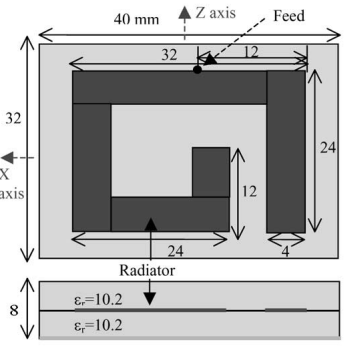
\includegraphics[scale=0.4]{./ContextoTecnologico/articulos/kim1}
    \caption{Diseño del parche radiante en forma de espiral de la antena microstrip descrita en \cite{kim}.}
    \label{fig:fig2.13}
\end{figure}

El diseño propuesto permite tener una antena mucho más peqeuña que otros diseños ya que la estructura en espiral, al igual que hemos visto en el ejemplo anterior, reduce el tamaño de la antena considerablemente. En cambio, se pierde eficiencia al no tener unas capas de substrato lo suficientemente anchas y grandes que permitan la radiación hacia el exterior.

A lo largo del artículo se hace un estudio sobre la comunicación entre la antena diseñada y otra externa tipo dipolo de media longitud de onda. La antena en espiral está situada en un torso humano diseñado en 3D, que podemos visualizar en la \textit{fig. \ref{fig:fig2.14}}.

Los resultados mostrados indican que el enlace de comunicaciones es posible de esta manera y que por supuesto cumplen con los límites legales de radiación máxima permitida para el cuerpo humano. Los autores concluyen argumentando que para este tipo de simulaciones en 3D del torso humano, es conveniente incluir parte del cuello y hombros, para obtener una correcta distribución de campos.

\vspace{1.5cm}

\begin{figure}[!htb]
    \centering
    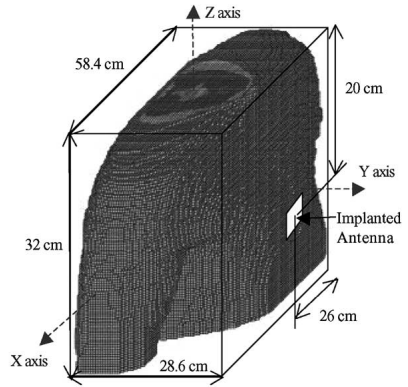
\includegraphics[scale=0.3]{./ContextoTecnologico/articulos/kim2}
    \caption{Diseño 3D del torso de cuerpo humano para simular la antena microstrip descrita en \cite{kim}.}
    \label{fig:fig2.14}
\end{figure}

Siguiendo la línea del anterior artículo, se diseña otra antena microstrip, pero esta vez con parche radiante en forma de serpentina en el artículo escrito por T. Karacolak et al. y titulado \textit{Design of a Dual-Band Implantable Antenna and Development of Skin Mimicking Gels for Continuous Glucose Monitoring}~\cite{karacola}. La gran diferencia con el anterior artículo se basa en que este nuevo diseño permite a la antena ser una antena dual, que trabaje tanto en la banda MICS, como en la banda ISM. Las dimensiones de la antena son reducidas de nuevo, obteniendo una antena apta para DMI.

\begin{figure}[!htb]
    \centering
    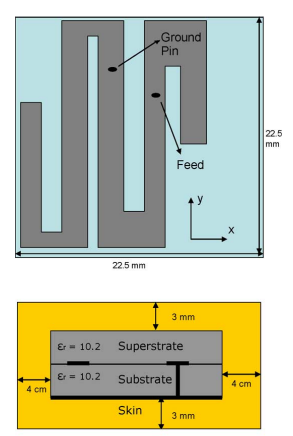
\includegraphics[scale=0.25]{./ContextoTecnologico/articulos/kara1}
    \caption{Diseño de la antena dual en forma de espiral descrita en \cite{karacola}.}
    \label{fig:fig2.15}
\end{figure}

\clearpage

La característica de la antena que le permite trabajar en las dos bandas es conseguida a través de diferencias en el parche radiante. En el anterior ejemplo~\cite{kim}, el ancho del parche era igual en toda su longitud, pero en este caso, se puede apreciar que hay distintos grosores a lo largo de la longitud. Sumando a esto, la antena posee un pin unido a tierra que hace cortocircuito para diferenciar cuándo empieza una banda y otra. En la \textit{fig. \ref{fig:fig2.16}} podemos apreciar estos detalles.

\begin{figure}[!htb]
    \centering
    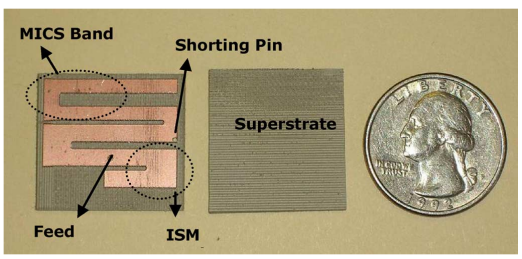
\includegraphics[scale=0.4]{./ContextoTecnologico/articulos/kara2}
    \caption{Antena dual fabricada basada en el diseño descrito en \cite{karacola}.}
    \label{fig:fig2.16}
\end{figure}

El artículo hace también un completo estudio sobre distintos geles que imitan a las propiedades el tejidos humanos para pruebas en la banda MICS. Los autores concluyen su artículo mostrando que la antena es eficiente en ambas bandas y cumplen su tarea a través de gráficas del parámetro $S_{11}$ y diagramas de radiación. Como línea futura, incluyen que están trabajando sobre un gel que funcione mejor para la banda ISM.

    \newpage \thispagestyle{empty} \cleardoublepage

%===============================================================
%PROPIEDADES Y BANDAS
%===============================================================
    \chapter{\textbf{Propiedades, modelos electromagnéticos del cuerpo humano y bandas de frecuencia}}\label{ch:cap3}

En este capítulo veremos una introducción a las propiedades electromagnéticas del cuerpo humano y las distintas bandas de frecuencia para Dispositivos Médicos Implantables. En la sección~\ref{sec:propiedades}, estudiaremos las propiedades y distintos modelos electromagnéticos del cuerpo humano. El análisis de las dos bandas principales de radiofrecuencia para los sistemas de comunicaciones de los DMI lo podemos ver en la sección~\ref{bandas}.


\section{Propiedades electromagnéticas y modelado del cuerpo humano}\label{sec:propiedades}

Antes de empezar a diseñar una antena microstrip, es importante conocer en qué entorno vamos a trabajar, es decir, sobre qué vamos a aplicar lo visto en el capítulo~\ref{ch:contexto}. En el presente estudio, dicho entorno es el \textbf{cuerpo humano}, el cual actúa de forma muy diferente con las diversas ondas electromagnéticas existentes. El cuerpo o tejidos humanos poseen propiedades electromagnéticas que pueden variar de forma sustancial, debido a que las ondas pueden variar tanto en amplitud, como en frecuencia, como en el modo en el que inciden en los tejidos. Es por esto, que los DMI junto a su sistema de comunicaciones, donde encontramos la antena microstrip, deben ser diseñados a la par que se dan las características del entorno de trabajo. Estas características de los tejidos son las que vamos a mencionar a continuación.

\subsection{Características de los tejidos humanos y/o animales}\label{subsec:caracteristicas-de-los-tejidos-humanos-y/o-animales}

Muchos autores han realizado estudios sobre las propiedades dieléctricas de los diferentes tejidos corporales, tanto humanos como animales, hasta la fecha. Existen datos tabulados~\cite{durney,geddes,stuchly} que van desde un rango de frecuencias desde 10 Hz hasta 30 GHz. Lo más difícil de estos estudios es siempre la tarea de conseguir tejidos o cuerpos vivos. La mayor parte de los recursos que se utilizan son organismos sin vida o tejidos muertos. En el caso de humanos, el estudio se centra en cadáveres a los que se les ha practicado la autopsia y en el caso de animales, son aquellos que se han sacados de mataderos: ovejas, cerdos, pollos, etc.

Para caracterizar un tejido animal o humano de manera electromagnética, tenemos tres importantes parámetros: la \textbf{permitividad relativa}, la \textbf{conductividad} y la \textbf{profundidad de penetración}.

\begin{itemize}
    \item La \textit{permitividad relativa} ($\epsilon_{r}$) hace referencia a cómo un campo eléctrico afecta a un medio y su tendencia a polarizarse: este parámetro es adimensional ya que se compara con la permitividad en el vacío ($\epsilon_{0}$). Se relaciona con el campo eléctrico y la densidad de flujo eléctrico de la siguiente manera:
    \begin{center}
        $D =  \epsilon E = \epsilon_{r}\epsilon_{0} E$
    \end{center}

    \item La \textit{conductividad} ($\sigma$) es la capacidad de un cuerpo para conducir corriente eléctrica, dejar paso a partículas cargadas: se mide en siemens por metro (S/m). El campo eléctrico es directamente proporcional a la distribución de corriente eléctrica gracias a esta magnitud:
    \begin{center}
        $J = \sigma E$
    \end{center}

    \item La \textit{profundidad de penetración} se definde como la longitud a la que las radiaciones electromagnéticas pueden llegar dentro de un material. Se mide simplemente en metros o milímetros y depende de los dos parámetros arriba mencionados, además de muchos otros, como la geometría del cuerpo, intensidad de la radiación, frecuencia, etc.
\end{itemize}

Podemos ver en la siguiente \textit{tabla \ref{tabla3.1}} extraída de \cite{yangtabla} algunos ejemplos de propiedades electromagnéticas de tejidos del cuerpo humano a una frecuencia de 2.45 GHz.

\begin{table}[h]
    \centering\scalebox{0.9}{
        \begin{tabular}{| c | c | c | c | c | c |}
            \hline
            \textbf{Nombre}       & \textbf{Conductividad} & \textbf{Permitividad} & \textbf{Profunidad}         \\
            \textbf{del tejido}   & \textbf{[S/m]}         & \textbf{relativa}     & \textbf{de penetración [m]} \\
            \hline
            \hline
            Cerebro, materia gris & 1.843                  & 48.83                 & 0.02031                     \\
            \hline
            Grasa                 & 0.10672                & 5.2749                & 0.11455                     \\
            \hline
            Músculo               & 1.773                  & 52.668                & 0.021886                    \\
            \hline
            Piel seca             & 1.4876                 & 37.952                & 0.022198                    \\
            \hline
            Piel húmeda           & 23.984                 & 20.369                & 0.0010736                   \\
            \hline
            Sangre                & 2.5878                 & 58.181                & 0.015842                    \\
            \hline
            \hline
        \end{tabular}}
    \caption{Propiedades electromagnéticas de tejidos humanos a 2.45 GHz.}
    \label{tabla3.1}
\end{table}

En la \textit{fig. \ref{fig:fig3.1}}, podemos ver la variación de los tres parámetros en músculo y grasa para un rango extenso de frecuencias.

\begin{figure}[!htb]
    \centering
    \subfigure[]{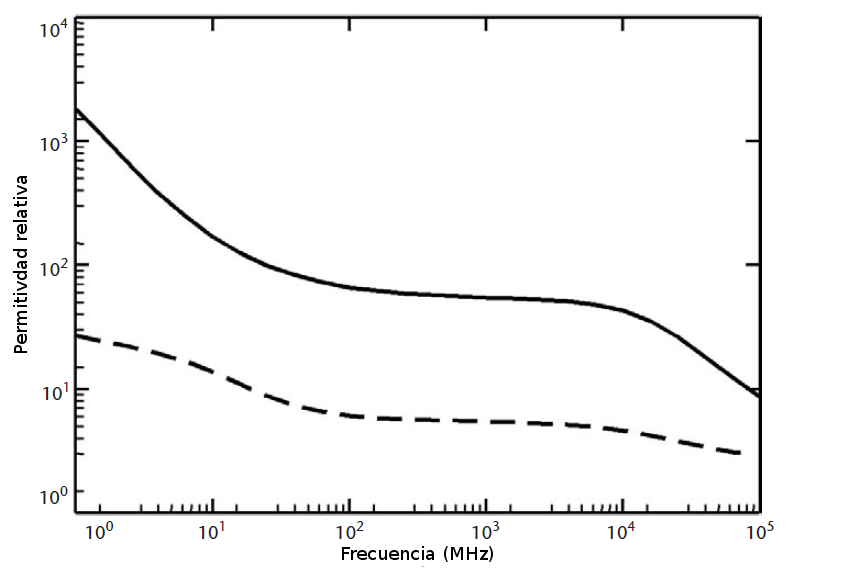
\includegraphics[scale=0.27]{./ContextoTecnologico/permitividad_relativa}}
    \subfigure[]{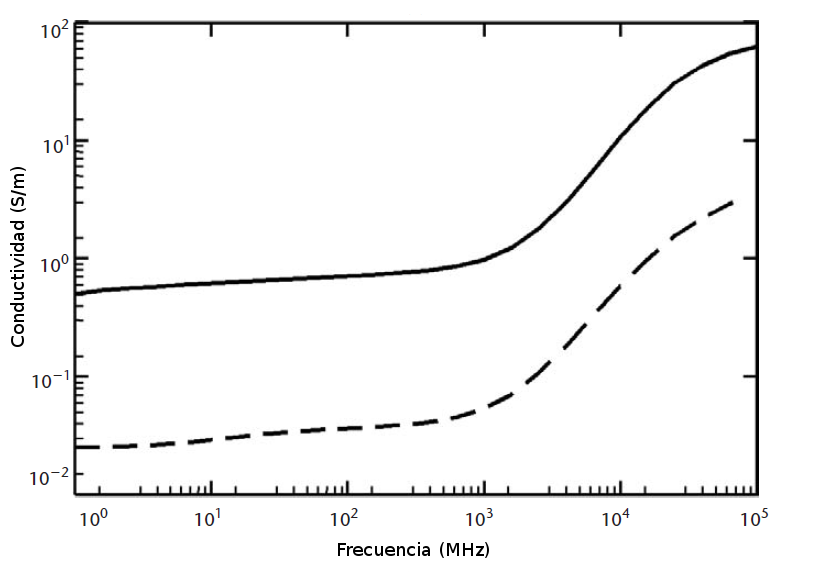
\includegraphics[scale=0.27]{./ContextoTecnologico/conductividad}}
    \subfigure[]{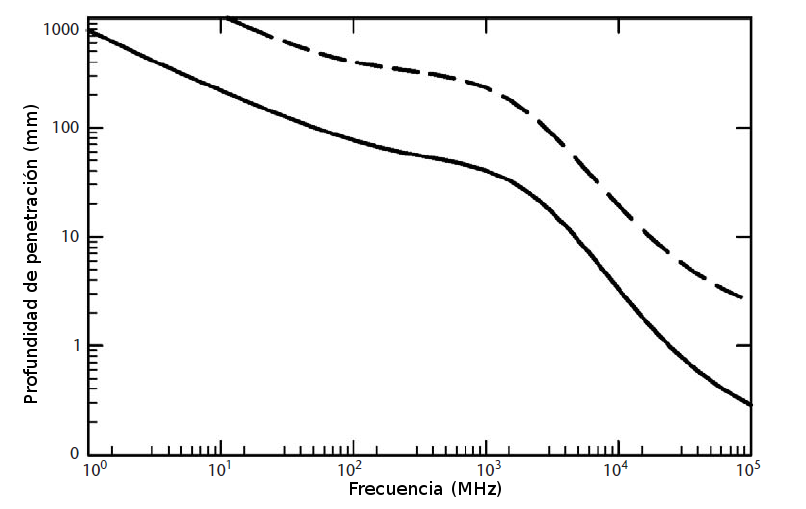
\includegraphics[scale=0.28]{./ContextoTecnologico/grado_de_penetracion}}
    \caption{Gráficas que representan distintas características de tejidos. En línea continua se representa el músculo y en discontinua grasa \cite{yang2}. En (a) permitividad relativa, en (b) conductividad y en (c) profundidad de penetración.}
    \label{fig:fig3.1}
\end{figure}

Las gráficas nos muestran una serie de características a destacar. Quedan recogidas en los siguientes puntos \cite{gabriel}:

\begin{itemize}
    \item La permitividad relativa de un tejido puede alcanzar valores de $10^{6}$ o $10^{7}$ para frecuencias menores de 100 Hz.
    \item Dicha permitividad decrece a altas frecuencias en tres principales puntos, conocidos como \textit{dispersiones $\alpha$, $\beta$} y \textit{$\gamma$}.
    \item La \textit{dispersión $\gamma$} que aparece en la región de los GHz, es debido a la polarización de las moléculas de agua.
    \item La \textit{dispersión $\beta$} que ocurre en torno a la región de los KHz, es debida principalmente a la polarización de las membranas celulares que actúan como barreras al paso de iones entre los medios intra y extra celular. Diversas contribuciones a esta dispersión vienen dadas por la polarización de proteínas o macromoléculas orgánicas.
    \item A bajas frecuencias, encontramos la \textit{dispersión $\alpha$} que está asociada con procesos de difusión iónica en la membrana celular.

\end{itemize}

Analizando la gráfica de la profundiad de penetración, se deduce la posibilidad de tener ondas capaces de viajar por el interior del cuerpo y ondas capaces de viajar por la superficie del mismo. La mayoría de los sistemas de comunicaciones de los DMI contemplan ambas posibilidades. Esto queda reflejado y se menciona en los dos estándares/bandas que podemos ver la sección \ref{bandas}: el estándar \textbf{MICS} (\textit{Medical Implant Communication Service}), que trabaja sobre los 402-405 MHz y la banda \textbf{ISM} (\textit{Industrial, Scientific and Medical band}) que trabaja sobre los 2.4 GHz.

\subsection{Modelos del cuerpo humano físicos para el estudio electromagnético}\label{subsec:modelos-del-cuerpo-humano-fisicos-para-el-estudio-electromagnetico}

Un modelo físico del estudio electromagnético o también conocido como \textbf{\textit{phantom}}, es un prototipo que se asemeja a alguna parte del cuerpo humano con propiedades parecidas a los tejidos biológicos que se tienen en dicha parte o sección \cite{yang}. El objetivo de los estuidos con \textit{phantoms} es analizar la influencia que crean los campos electromagnéticos con el cuerpo a analizar. Estos \textit{phantoms} son esenciales en muchos experimentos e investigaciones para probar dispositivos tecnológicos y cuantificar su seguridad para la salud del ser humano. Para cuantificar esa seguridad se utiliza el índice de absorción específica o SAR (\textit{specific absortion rate}), el cual mide cuántos W/Kg son absorbidos por el cuerpo. Todos los dispositivos actuales que emiten en bandas de RF (radiofrecuencia) son sometidos a estudios de SAR para medir este índice, el cual debe estar bajo un límite propuesto internacionalmente para cada banda. Los límites SAR son actualmente fijados por ANSI \cite{ANSI}, IEEE \cite{IEEE} e ICNIRP \cite{ICNIRP}.

La clasificación más común para los \textit{phantoms} depende de su estado físico final, es decir, una vez construido, de qué manera, material o forma se ha realizado. Así, tenemos los \textit{phantoms} líquidos, los \textit{phantoms} de gel o semisólidos y los \textit{phantoms} sólidos o secos.

\subsubsection{\textit{Phantoms} líquidos}

Los \textit{phantoms} líquidos son los más antiguos. Consisten básicamente en un recipiente relleno de líquido con las mismas características o propiedades del tejido humano que se analiza en un determinado rango de frecuencias. Son usados en su gran mayoría para los estudios SAR aunque poseen la desventaja de no poder tomar medidas cerca de la superficie del objeto, únicamente en el interior.

\subsubsection{\textit{Phantoms} de gel o semisólidos}

Los \textit{phantoms} de gel o semisólidos son adecuados para medir campos en tejidos con gran catidad de agua, como el tejido muscular, el tejido cerebral, etc. y ajustar sus característcias eléctricas en un amplio espectro de frecuencias.

\subsubsection{\textit{Phantoms} sólidos o secos}

Los \textit{phantoms} sólidos son utilizados cuando no se han realizado las medidas oportunas en la superficie del cuerpo de estudio. Dichos \textit{phantoms} son hechos de materiales que son capaces de mantener su forma en un extenso periodo de tiempo. De esta manera, las medidas SAR son realizadas a través de termografía: el aumento de temperatura que aparece en la superficie del \textit{phantom} después de una serie de exposiciones a campos electromagnéticos da lugar a una medición SAR.

A continuación, podemos observar diferentes modelos que se han usado en estudios de medidas SAR, todos con forma o apariencia humana.

\begin{figure}[!htb]
    \centering
    \subfigure[]{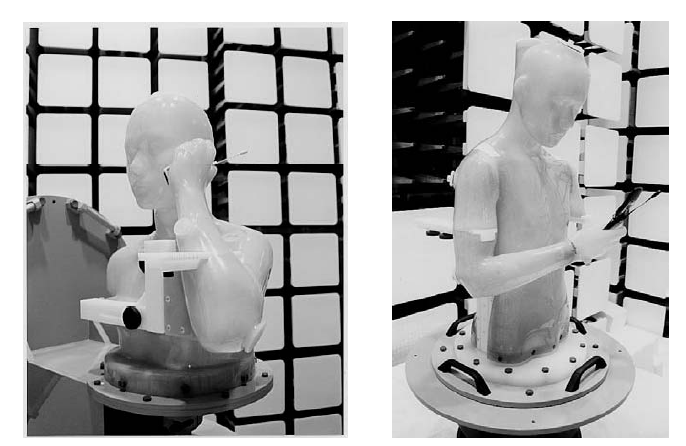
\includegraphics[scale=0.3]{./ContextoTecnologico/phantoms}}
    \subfigure[]{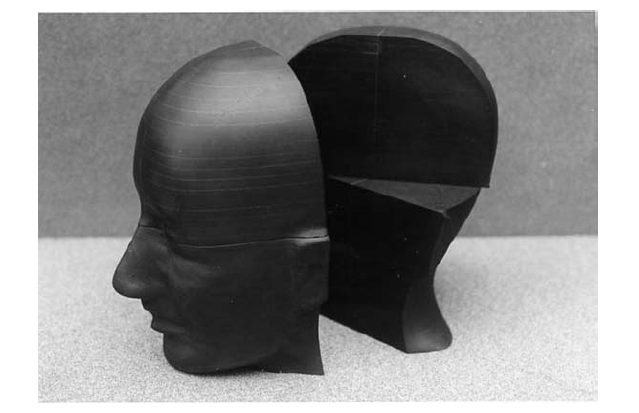
\includegraphics[scale=0.3]{./ContextoTecnologico/dry_phantom}}
    \caption{Distintos modelos de phantoms con apariencia humana \cite{yang}. En (a) modelos con posturas realistas humanas usando un teléfono móvil: a la izquierda en posición de conversación y a la derecha en posición de vista. En (b) un ejemplo de phantom seco.}
    \label{fig:fig3.2}
\end{figure}

\subsection{Modelos del cuerpo humano númericos para el estudio electromagnético}\label{subsec:modelos-del-cuerpo-humano-numericos-para-el-estudio-electromagnetico}

Para llegar a realizar un estudio exhaustivo de la medición registrada en un cuerpo, no sólo es necesario la creación de \textit{phantoms} o modelos físicos. Se necesitan estudios realizados por ordenador mediante medidas numéricas que contrasten los datos físicos obtenidos. En la actualidad, estos modelos numéricos son ampliamente utilizados a la par que los modelos físicos, ya que proporcionan un número importante de datos. Su principal fuente son los \textit{vóxels}. Un \textbf{\textit{vóxel}} es un píxel en tres dimensiones que representa la unidad mínima para la creación de modelos numéricos realizados por computador.

\begin{figure}[!htb]
    \centering
    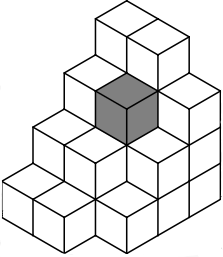
\includegraphics[scale=0.3]{./ContextoTecnologico/voxel}
    \caption{Ejemplo de vóxel cúbico. \cite{voxel}}
    \label{fig:fig3.3}
\end{figure}

Un vóxel forma parte de una matriz tridimensional necesaria para el procesamiento de imágenes. En nuestro caso, forman las imágenes que se usarán posteriormente para construir un modelo del cuerpo humano tridimensional. Los \textit{vóxels} pueden contener numerosos datos escalares que ayudan al posicionamiento, a calcular el volumen de la figura, etc.

En el campo de los DMI para personas, los \textit{voxel phantoms} ayudan a calcular las características de las antenas de los DMI cuando están cerca del cuerpo humano, formando un modelo real numérico, de gran exactitud y precisión.

\begin{figure}[!htb]
    \centering
    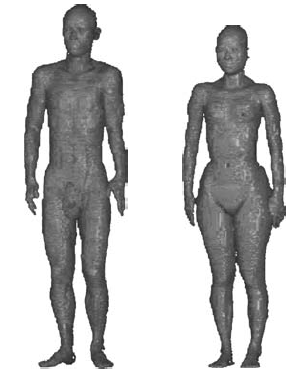
\includegraphics[scale=0.30]{./ContextoTecnologico/voxel_phantoms}
    \caption{Voxel phantoms de alta resolución de cuerpo entero. Modelos japoneses hombre y mujer. \cite{nagaoka}}
    \label{fig:fig3.4}
\end{figure}

\subsubsection{Técnicas para modelos numéricos para comunicaciones wireless}

Los modelos numéricos también se utilizan para el cálculo de índices SAR, pero también son utilizados como herramienta en análisis a frecuencia de microondas \cite{yang1}. Estos modelos permiten además aproximaciones semianalíticas, suponiendo que el cuerpo es un medio dieléctrico con pérdidas; esto da lugar a diversas técnicas de estudio:

\begin{itemize}
    \item  \textbf{Teoría geométrica uniforme de difracción} (\textit{Uniform Geometrical Theory of Diffraction, UTD}). Se basa en óptica geométrica y en teoría de difracción.
    \item  \textbf{Técnica de trazo de rayos o RT}. Puede ser usada para determinar la fuerza de la señal recibida y perfiles de potencia en situaciones donde la longitud de onda es pequeña en relación con el tamaño del entorno de propagación.
    \item \textbf{Método de los momentos o MoM}. Es una técnica para resolver ecuaciones con integrales complejas reduciéndolas a un sistema de ecuaciones lineales más simple. Puede ser usada en el dominio tanto de la frecuencia como del tiempo para analizar de manera bastante exacta estructuras estrechas.
    \item \textbf{Método de los elementos finitos o FEM}. La idea básica de esta técnica es dividir las estructuras electromagnéticas en un número de elementos de forma variante, tales como rectangulares o triangulares. Cada elemento tiene un valor de campo asociado, los cuales conforman una matriz de pesos donde calcular autovalores.
    \item \textbf{Método de las diferencias finitas en el dominio del tiempo o FDTD Method}. Método que destacaremos a continuación ya que es implementado por el software que vamos a utilizar para nuestro estudio.
\end{itemize}

\subsubsection{Método de las diferencias finitas en el dominio del tiempo. FDTD Method}

Este método es uno de los más conocidos dentro de los métodos numéricos para problemas de condiciones de contorno difíciles de resolver. Ha sido aplicado además a problemas electromagnéticos durante muchos años~\cite{yang}. Al igual que FEM, parte de la divisón de estructuras electromagnéticas en un conjunto de pequeñas celdas para poder así obtener de manera idónea los cálculos de condiciones de contorno complicados en medios no homogéneos.

Una de las razones por las cuales el método FDTD ha visto un rápido crecimiento en su uso, ha sido su complejidad en pasos de computación\footnote{Número de instrucciones necesarias de un programa para realizar un cálculo computacional.}, siendo esta O(n). Otros métodos, como el MoM o FEM, necesitan O(n$^{2}$) de complejidad, es decir, necesitan n veces más cálculos computacionales que en FDTD. Los resultados con un rango de frecuencias amplio, se pueden conseguir fácilmente a través de la implementación de la Transformada Rápida de Fourier (FFT) en el dominio temporal, lo que abarata el cálculo de los datos a obtener~\cite{yang}.

Sin embargo, el FDTD tiene sus inconvenientes. Requiere que todo el dominio de trabajo sea dividido en una malla compuesta por celdas, las cuales deben ser más pequeñas que la longitud de onda más corta y más pequeñas que la medida más diminuta del modelo. Además, como muchos de los elementos estructurales electromagnéticos son curvos, los límites o perfiles de las celdas no serán suaves, sino rugosas, con cortes. En este aspecto, el método FDTD no es tan flexible como el FEM.


\section{Bandas de frecuencia para los sistemas de comunicación de los dispositivos médicos implantables}\label{bandas}

En los capítulos~\ref{ch:intro} y~\ref{ch:contexto} se ha mencionado que la tecnología utilizada en los orígenes de los DMI para que los dispositivos se comunicaran, era el enlace inductivo. Debido a sus limitaciones en capacidad y distancia de transmisión de datos, se han establecido dos bandas certificadas de radiofrecuencia para DMI que minimizan esas dos limitaciones. Nos referimos a la banda \textbf{MICS} (\textit{Medical Implant Communication Service}) y la banda \textbf{ISM} (\textit{Industrial, Scientific and Medical band}).

\subsection{Banda MICS}

Tanto el Instituto Europeo de Estandarizaciones en Telecomunicación, conocido como ETSI (\textit{European Telecommunications Standards Institute}), como el FCC (\textit{Federal Communications Commission}) por parte de Estados Unidos, recogen la estandarización de la banda MICS~\cite{mics}. Nos centraremos principalmente en el estándar definido en ETSI, el cual establece dos principales usos para esta banda:

\begin{itemize}
    \item La comunicación entre un dispositivo implantable y un dispositivo que funciona como estación base que recoge la información que vierte el primero.
    \item La comunicación entre varios (dos o más) dispositivos que se encuentran implantados en un mismo cuerpo.
\end{itemize}

Sin embargo, el estándar no recoge otro uso también destacable y que es posible realizar: la comunicación entre dispositivos implantables que se sitúan en diferentes cuerpos~\cite{yang9}.

La frecuencia de trabajo de esta banda se encuentra entre los \textbf{402 MHz} y los \textbf{405 MHz}. Este espectro de 3 MHz se reparte en 10 canales, con lo que el máximo ancho de banda disponible es de 300 KHz en una única transmisión. Esto es una desventaja importante para esta banda ya que si se trabaja en comunicaciones \textit{full-duplex}, es decir todo dispositivo puede transmitir y recibir información a la vez, el ancho de banda necesario para cada dispositivo es pequeño, lo que reduce la tasa de información considerablemente. Debido a esto, tenemos otra posibilidad para utilizar todo el ancho de banda: utilizar \textit{half-duplex}, es decir que en cada momento el dispositivo sólo puede transmitir o recibir información (no a la vez), y que cada dispositivo utilice totalmente el ancho de banda en su turno de transmisión. Esta última posibilidad limita tanto la recogida de información como la comunicación entre dispositivos.

Como los 300 KHz de ancho de banda total en esta banda supone una restricción importante, se ha establecido que en los límites de emisión, la potencia debe ser 20 dB menor que el máximo nivel. La potencia radiada equivalente\footnote{El nivel máximo de campo emitido en cualquier dirección debería ser igual o menor a la de un dipolo resonante a la misma distancia con máxima directividad siendo alimentado por una señal de 25$\mu$W.} (ERP) es de 25$\mu$W. Según el estándar MICS para ETSI~\cite{mics} los niveles de ERP deben medirse a través de simulaciones recogidas en implantes colocados sobre un objeto con forma de torso humano. No existen estandarizaciones para implantes usados principalmente en otras partes del cuerpo, como son brazos, piernas o en la cabeza. De acuerdo con el estándar, cada implante diseñado y fabricado en esta banda, sin importar dónde irá colocado, debe ser probado con la misma simulación de torso humano anteriormente descrita.

Existe otro inconveniente para esta banda de frecuencias. El Servicio de Apoyo Meteorológico o METAIDS (\textit{Meteorological Aids Service}), utiliza esta banda para transmitir información de la previsión meteorológica desde antenas colocadas en globos aerostáticos hasta antenas que recogen la información en la superficie de la Tierra. Por esta razón, la banda MICS está especificada únicamente para su uso en interiores y no para su uso en exteriores~\cite{yang9,mics}. Posteriormente, la ITU-T ha propuesto una recomendación de cómo debe repartirse y usarse el espectro en la banda de 401 MHz a 406 MHz~\cite{itut}, en el cual la banda MICS queda dispuesta entre los 402 MHz y los 405 MHz: el resto es para el servicio METAIDS.

\subsection{Banda ISM}\label{subsec:banda-ism}

La banda ISM es usada también para la comunicación entre implantes o DMI. Trabaja en las mismas frecuencias que algunos estándares de IEEE~\cite{IEEE} como el 802.11 (Wi-Fi)~\cite{wifi}, 802.15 (Bluetooth)~\cite{bluetooth} por poner unos ejemplos.

De acuerdo de nuevo a ETSI~\cite{etsi}, el máximo ERP en la banda ISM es de 100 mW. Las tecnologías de reparto de frecuencias que son posibles de utilizar en esta banda son espectro ensanchado, espectro ensanchado por salto de frecuencias o FHSS y espectro ensanchado por secuencia directa o DSSS. La banda de frecuencias se encuentra entre los 2.4 y los 2.4835 GHz.

La desventaja fundamental de esta banda de trabajo es el solapamiento que existe con otros estándares y tecnologías: esto hace que sea una banda con riesgos en seguridad e interoperabilidad. Con respecto a la banda MICS, que trabaja en torno a los 400 MHz como hemos mencionado antes, la atenuación de las ondas de propagación que presentan en la banda ISM ante un cuerpo humano es mucho mayor. De esta manera, esta banda es posible utilizarla para el uso de dispositivos implantados alrededor del cuerpo y no en su interior, ya que se aprovecha de las ondas que se propagan por la superficie del cuerpo~\cite{conway,yang9}. El caso más general, es utilizar esta banda para sincronizar y activar al DMI cuando se vaya a interactuar con él; es entonces cuando se utiliza la banda MICS para intercambiar información. Un ejemplo claro lo podemos ver en la siguiente sección.

Sin embargo, el problema al que hacíamos mención en la banda MICS, el poco ancho de banda disponible, aquí es solventado, ya que tenemos un ancho de banda muy superior. Dos o más dispositivos pueden transmitir a la vez, pueden establecerse comunicaciones \textit{full-duplex} sin problemas junto a la utilización además de cualquier tecnología de las arriba citadas, FHSS, DSSS, etc., con lo que tenemos la posibilidad de aumentar los recursos de estos dispositivos.

\subsection{Comparación entre las bandas MICS e ISM}\label{subsec:comparacion}

En la \textit{tabla \ref{tab:tabla3.2}} se presenta una tabla comparativa de ambos estándares, donde se recogen las bandas de frecuencia, usos, potencia, tipo de comunicación, etc.

\begin{table}[h]
    \centering\scalebox{0.8}{
        \begin{tabular}{| c | c | c | c | c | c |}
            \hline
            \large{\textbf{Estándar}}           & \textbf{MICS}               & \textbf{ISM}                     \\
            \hline
            \hline
            \large{\textbf{Frecuencias}}        & 402 - 405 MHz               & 2.4 - 2.4835 GHz                 \\
            \large{\textbf{de trabajo}}         &                             &                                  \\
            \hline
            \large{\textbf{Potencia}}           & 25 $\mu$W                   & 100 mW                           \\
            \large{\textbf{máxima}}             &                             &                                  \\
            \hline
            \large{\textbf{Recogido}}           & ITU-T                       & ITU-T                            \\
            \large{\textbf{en}}                 & ETSI                        & ETSI                             \\
            & FCC                         & FCC                              \\
            %\hline
            %\large{\textbf{Uso}} & Tejidos interior del cuerpo & Tejidos superficiales del cuerpo \\
            %\large{\textbf{científico/médico}} & & \\
            \hline
            \large{\textbf{Velocidad}}          & Kbps                        & Mbps                             \\
            \large{\textbf{de bits}}            &                             &                                  \\
            \hline
            \large{\textbf{Ancho}}              & 300 KHz                     & MHz                              \\
            \large{\textbf{de banda}}           &                             &                                  \\
            \hline
            \large{\textbf{Tipo}}               & \textit{half-duplex}        & \textit{full-duplex}             \\
            \large{\textbf{de transmisión}}     &                             &                                  \\
            \hline
            \large{\textbf{Reparto}}            & N/A                         & FHSS, DSSS                       \\
            \large{\textbf{de frecuencias}}     &                             &                                  \\
            \hline
            \hline
        \end{tabular}}
    \caption{Características comparativas de las bandas MICS e ISM vistas anteriormente.}
    \label{tab:tabla3.2}
\end{table}

Como ejemplo práctico a las dos bandas vistas, podemos ver un modelo de chip de la empresa \textbf{\textit{Microsemi}}, antigua \textit{Zarlink Semiconductor}. En la ilustración de la \textit{fig. \ref{fig:fig3.5}} se puede ver. Este modelo utiliza la banda ISM para \textit{despertar} al dispositivo implantable que está junto al chip: el dispositivo entra en modo \textit{idle} o inactivo cuando después de un cierto tiempo no recibe ninguna orden de algún dispositivo externo. Una vez despertado, el dispositivo recoge toda la información necesaria por el uso de la banda MICS y utiliza esta misma banda para enviar dicha información al dispositivo externo que le ha despertado. En definitiva:

\begin{itemize}
    \item El equipo externo de monitorización manda una señal en la banda ISM al dispositivo del chip para que se active y empiece a funcionar.
    \item El dispositivo del chip, recoge la información a través de la banda MICS y la entrega al equipo externo por la misma vía.
\end{itemize}

\begin{figure}[!htb]
    \centering
    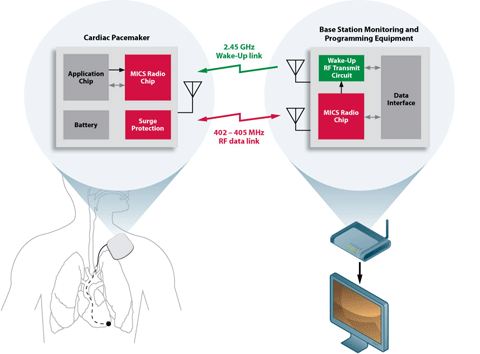
\includegraphics[scale=0.6]{./Introduccion/medical-cardicpacemaker}
    \caption{Ilustración ejemplo de la estructura de comunicación de un chip de la empresa \textit{Microsemi} \cite{zarlink}.}
    \label{fig:fig3.5}
        % http://www.zarlink.com/zarlink/hs/22122.htm
\end{figure}

    \newpage \thispagestyle{empty} \cleardoublepage

%===============================================================
%METODOLOGÍA
%===============================================================
    \chapter{\textbf{Metodología}}\label{ch:metodos}

La herramienta de trabajo principal que vamos a utilizar a lo largo de nuestro estudio es el software \textbf{\textit{CST Studio Suite 2010}}, el cual permite realizar simulaciones de antenas con sus resultados de ganancia, directividad, campos y diversas medidas. Entraremos en detalle en este capítulo en el principal uso que le vamos a dar: diseñar y simular antenas microstrip.


\section{Introducción al software CST}

El software CST proviene de las siglas de \textit{Computer Simulation Technology} el cual es un programa que permite diseñar y simular aplicaciones para filtros, conectores, antenas, capacitores, inductancias, guías de onda y un sinfín de dispositivos que se pueden modelar~\cite{cst}.

\begin{figure}[!htb]
    \centering
    
\includegraphics[scale=0.35]{./Metodologia/CST_Intro}
    \caption{Logo del programa CST Studio Suite 2010.}
    \label{fig:fig4.1}
\end{figure}

Una vez iniciado el programa tenemos la posibilidad de elegir el tipo de problema al que nos vamos a enfrentar, es decir, podemos elegir de qué manera va a ir encaminado nuestro proyecto, ya que si elegimos una opción u otra, las condiciones en las que trabajaremos serán muy distintas. Como podemos ver en la \textit{fig. \ref{fig:fig4.2}}, se nos presentan ocho opciones a elegir, desde un proyecto que engloba un estudio electromagnético, pasando por un estudio de partículas o incluso un estudio de conectores o de líneas microstrip.

\begin{figure}[!htb]
    \centering
    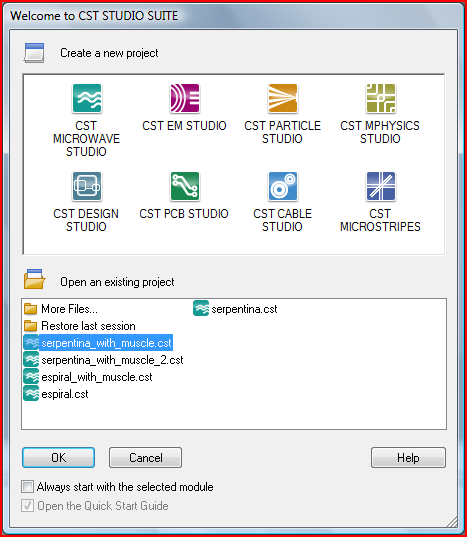
\includegraphics[scale=0.45]{./Metodologia/CST_Open_folder}
    \caption{Ventana introductoria del CST Studio Suite 2010.}
    \label{fig:fig4.2}
\end{figure}

En el marco en el que nos encontramos, de todas esas opciones la elegida por nosotros será \textbf{CST MICROWAVE STUDIO}, es decir, un proyecto en el que se diseñan y simulan dispositivos que trabajan a frecuencas de microondas, como los teléfonos móviles, dispositvos aeronáuticos o como en nuestro caso, antenas planas o de parche.

\subsection{Entorno de trabajo del software CST}\label{subsec:entorno-de-trabajo-del-software-cst}

Después de elegir el tipo de proyecto en el que nos vamos a embarcar, el programa nos presenta una interfaz como la que podemos ver en la \textit{fig. \ref{fig:fig4.3}} bastante clara e intuitiva. En la parte de arriba, tenemos todas las herramientas a nuestra disposición para diseñar, fijar parámetros de nuestra antena y simular según unas condiciones. En la parte de la izquierda se recogen en un árbol de directorios todos los elementos de nuestro diseño, desde componentes, pasando por los materiales utilizados hasta las propias simulaciones y resultados en último lugar. En la parte de abajo, tenemos las variables globales que se pueden definir como queramos para facilitar la tarea de asignar valores a las medidas del diseño en proceso. Y por último, en la parte central, tenemos la aparencia de nuestro diseño en un entorno tridimensional.

\begin{figure}[!htb]
    \centering
    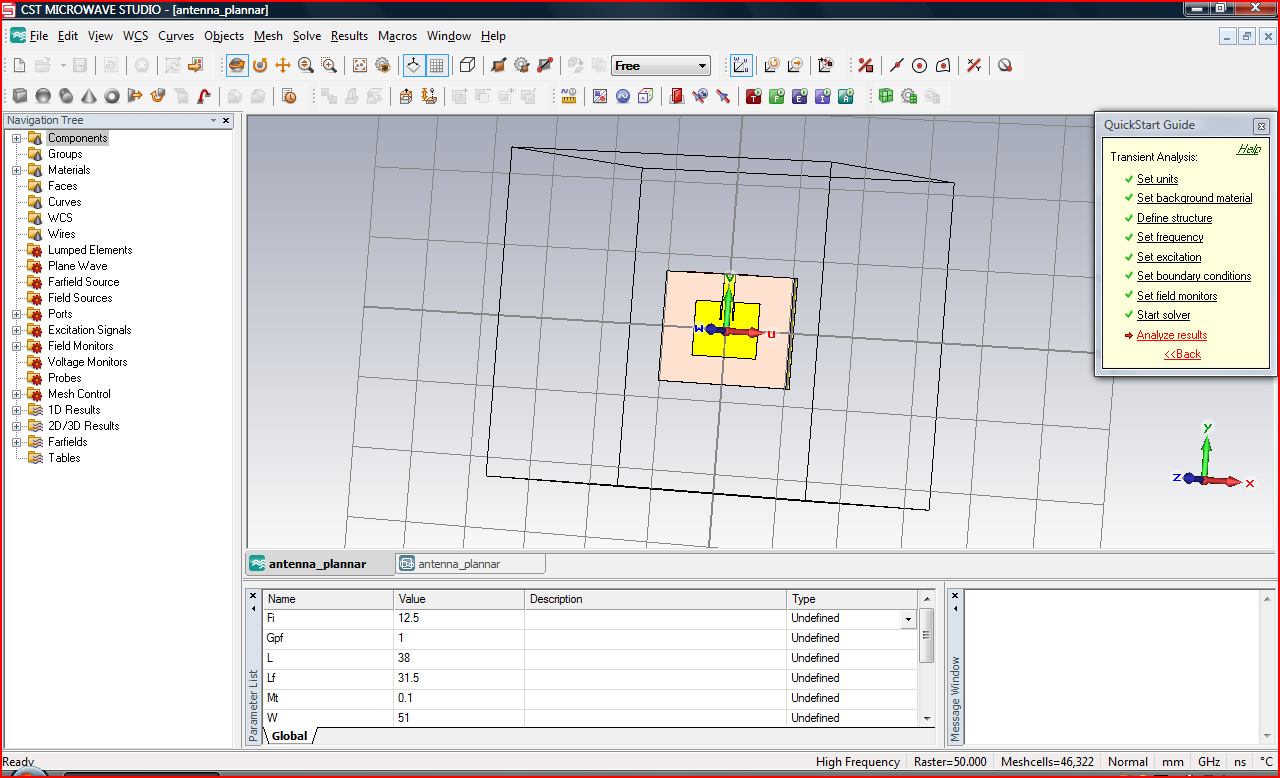
\includegraphics[scale=0.35]{./Metodologia/CST_first_window}
    \caption{Entorno de trabajo del CST Studio Suite 2010.}
    \label{fig:fig4.3}
\end{figure}

\subsection{Diseño antena ejemplo en CST}\label{subsec:diseno-antena-ejemplo-en-cst}

Lo primero que debemos hacer es dar información al CST sobre las medidas del diseño. Para ello tenemos la opción de crear variables globales con las que podremos dar forma a la antena, como por ejemplo, el largo y ancho, la altura del substrato o la longitud de la alimentación.

\clearpage

\begin{figure}[!htb]
    \centering
    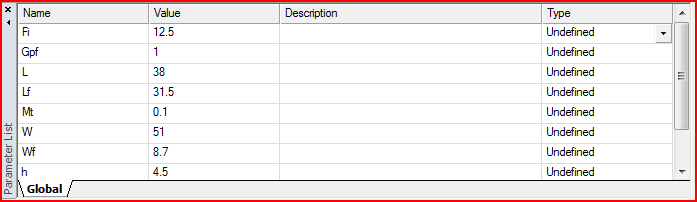
\includegraphics[scale=0.4]{./Metodologia/CST_global_parametres}
    \caption{Parámetros globales para el CST.}
    \label{fig:fig4.4}
\end{figure}

Una vez introducidas las variables globales, es el turno de construir nuestro diseño de la antena. En la barra de herramientas superior tenemos una serie de botones con distintas formas geométricas que se usan para crear las diferentes partes de la antena en tres dimensiones: cubos, hexaedros, conos, cilindros, toroides, etc. Existe incluso la opción de crear capas a partir de las ya creadas con la opción de \textit{extrude}.

\begin{figure}[!htb]
    \centering
    
\includegraphics[scale=0.7]{./Metodologia/CST_figures}
    \caption{Herramientas para la creación del dispositivo.}
    \label{fig:fig4.5}
\end{figure}

El paso siguiente a elegir el tipo de material de cada capa y sus correspondientes medidas, además de colocar adecuadamente la alimentación. Dicha alimentación puede ser un puerto discreto, simplemente unir conductor y dieléctrico o como una guía de onda, en la que tendremos que especificar las dimensiones de la misma. Dependiendo de dónde lo alimentemos y cómo, tendremos unos u otros resultados.

Cuando hayamos completado nuestro diseño procederemos a la etapa de simulación, la cual es clave en todo proyecto realizado en este software. Tenemos en primer lugar que elegir qué característica queremos medir: campo electromagnético, flujo magnético, corriente, etc. Esto se ve en \textit{fig. \ref{fig:fig4.6}}, que representa la ventana de \textit{monitor}.

\clearpage

\begin{figure}[!htb]
    \centering
    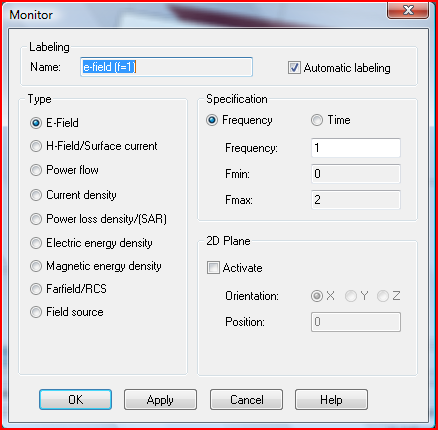
\includegraphics[scale=0.45]{./Metodologia/CST_monitor}
    \caption{Ventana \textit{monitor} con las distintas simulaciones y pruebas posibles.}
    \label{fig:fig4.6}
\end{figure}

El siguiente paso es ejectuar las tareas de simulación a través de la herramienta \textit{solver}. Elegimos de qué manera queremos que salgan los resultados, cuánta impedancia hay a la entrada, etc. y después tendremos los datos listos para revisarlos.

\begin{figure}[!htb]
    \centering
    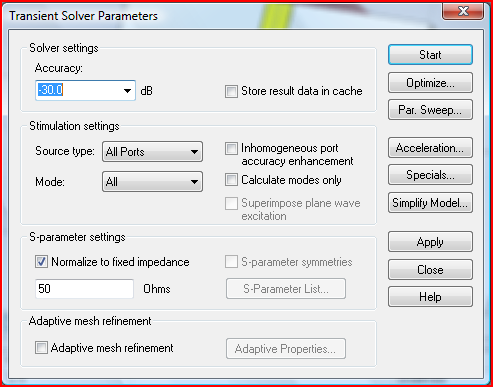
\includegraphics[scale=0.45]{./Metodologia/CST_solver}
    \caption{Ventana \textit{solver} con los parámetros disponibles para la simulación.}
    \label{fig:fig4.7}
\end{figure}

La última parte en la tarea del manejo del software CST será comprobar el diseño y las simulaciones conseguidas. En las siguientes imágenes podemos ver para un ejemplo concreto de antena microstrip, sus distintos resultados.

\clearpage

\begin{figure}[!htb]
    \centering
    \subfigure[]{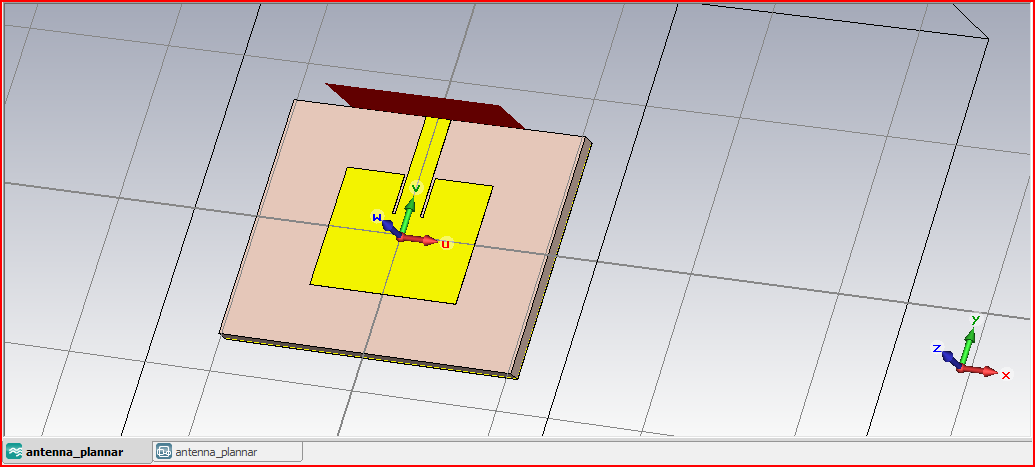
\includegraphics[scale=0.3]{./Metodologia/CST_antenna}}
    \subfigure[]{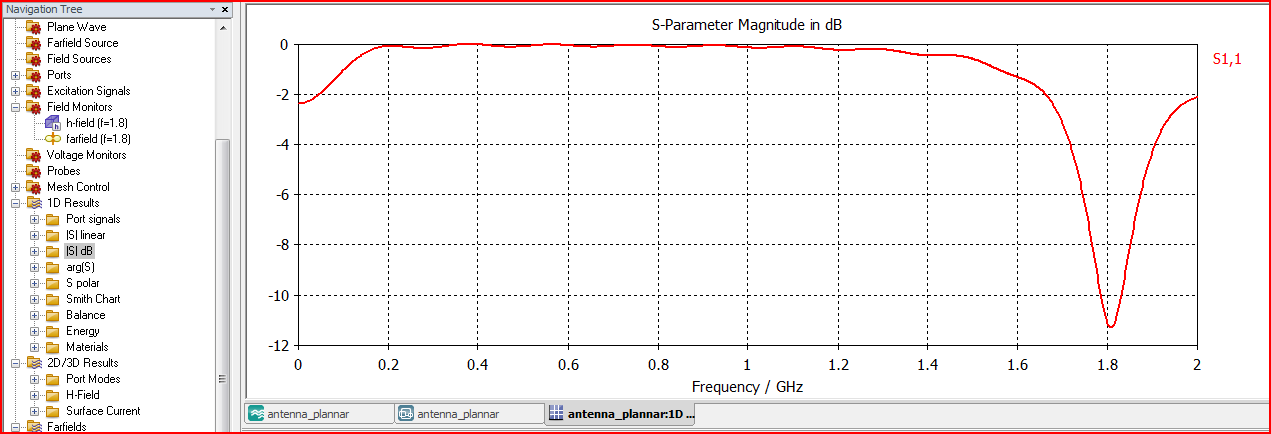
\includegraphics[scale=0.3]{./Metodologia/CST_dB}}
    \subfigure[]{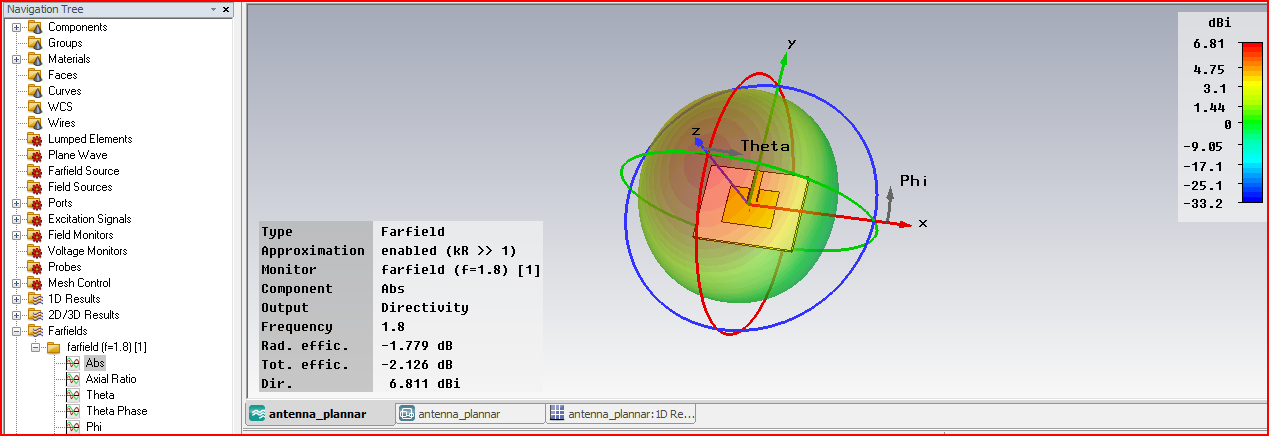
\includegraphics[scale=0.3]{./Metodologia/CST_farfield}}
    \caption{Imágenes tras el diseño y simulación de una antena ejemplo en el CST. En (a) un diseño final en 3D de una antena. En (b) gráfica del parámetro $S_{11}$. En (c) diagrama de radiación en 3D.}
    \label{fig:fig4.8}
\end{figure}

\clearpage


\section{Matlab como herramienta de apoyo}\label{sec:matlab-como-herramienta-de-apoyo}

El software \textbf{\textit{Matlab R2010b}} ha sido utilizado para crear las gráficas de los parámetros $S_{11}$ de las distintas simulaciones, además de las gráficas comparativas entre simulaciones del mismo parámetro.

Para ello, se ha obtenido del software CST los datos tabulados de cada simulación del parámetro $S_{11}$ por medio de un fichero de texto, el cual se ha metido como entrada un fichero \textbf{.m} de Matlab que se ha creado para este propósito.

\begin{figure}[!htb]
    \centering
    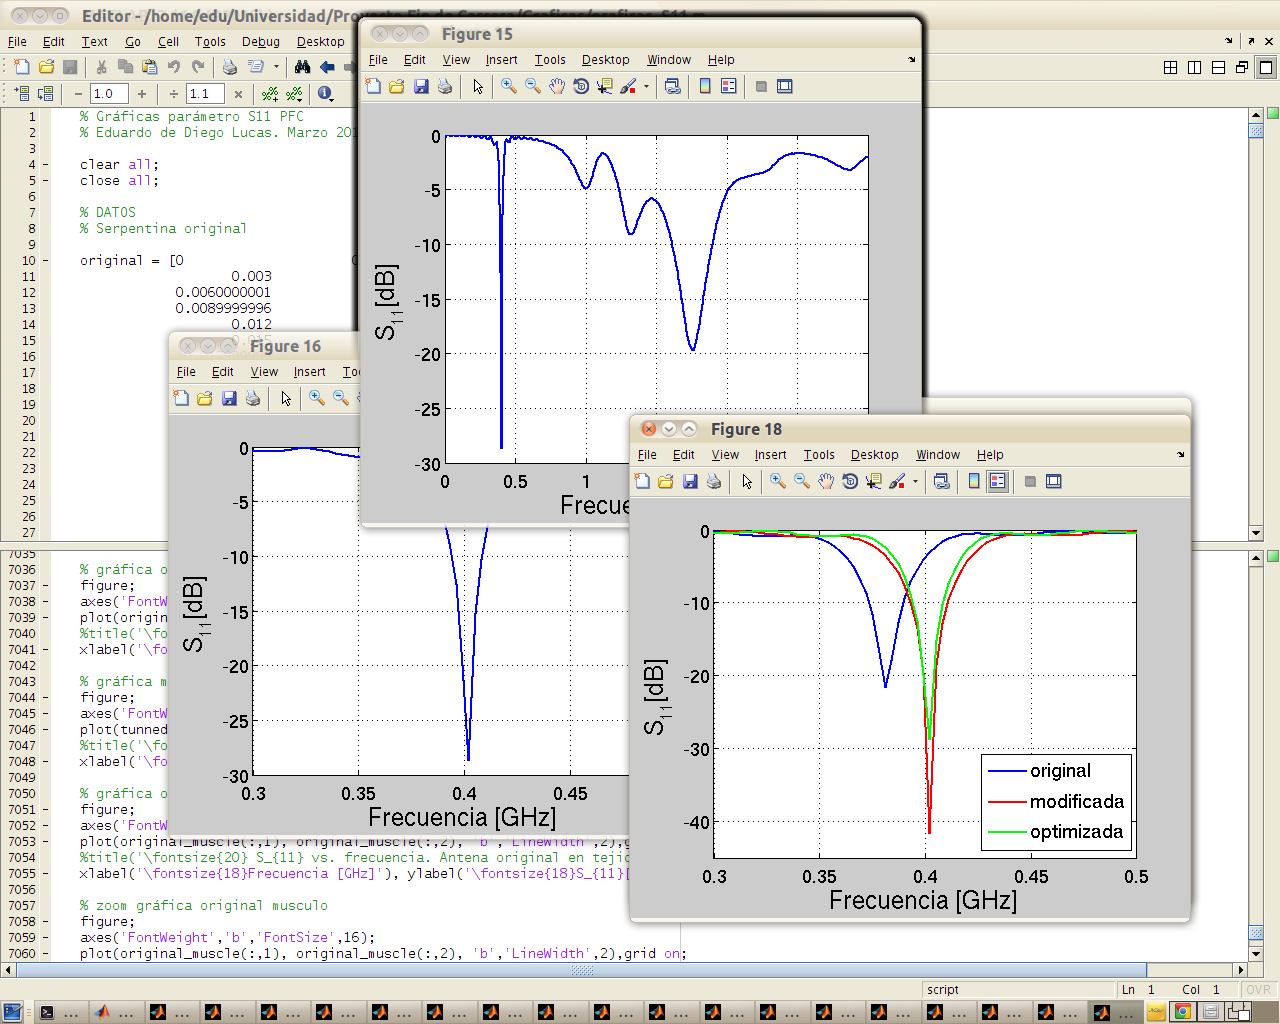
\includegraphics[scale=0.35]{./Metodologia/matlab2}
    \caption{Programa Matlab y su editor con distintas gráficas obtenidas del archivo creado.}
    \label{fig:fig4.9}
\end{figure}
    \newpage \thispagestyle{empty} \cleardoublepage

%===============================================================
%SIMULACIONES
%===============================================================
    \chapter{\textbf{Simulaciones de antenas microstrip en forma de serpentina}}\label{ch:simulaciones}

En este capítulo presentaremos la antena de tecnología microstrip con parche radiante en forma de serpentina descrita en el artículo de Soontornpipit~\cite{soont}. En las secciones~\ref{sec:base} y~\ref{sec:original} veremos el análisis y simulación de la antena original del artículo. A continuación, veremos en la sección~\ref{sec:modificado} un diseño modificado de la antena original ajustando algunos parámetros. En último punto, la sección~\ref{sec:optimizado}, analizaremos y simularemos una antena con materiales que se encuentran habitualmente en laboratorios de investigación y con algunos parámetros optimizados a partir del diseño original.


\section{Introducción al diseño base de la antena}\label{sec:base}

Comenzaremos explicando el diseño original del artículo de Soontornpipit. En este artículo el diseño de la antena es muy simple: se trata de una antena microstrip, alimentada por un cable coaxial y que posee una estructura radiante en forma de serpentina, es decir, tiene los brazos plegados entre sí formando varias curvas en ángulo recto. Las dimensiones originales del diseño del parche están recogidas en la \textit{fig. \ref{fig:fig5.1}}. La medida $B$ del último brazo de la estructura de serpentina la toman los autores del artículo como una variable a estudiar a lo largo del mismo. Para nuestro estudio hemos cogido la medida inicial de $B$ que toma el valor de 8.4 mm.

\begin{figure}[!htb]
    \centering
    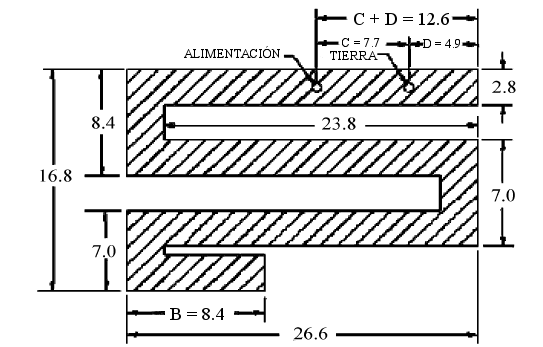
\includegraphics[scale=0.55]{./Simulaciones/original_design2}
    \caption{Medidas originales del diseño de Soontornpipit \cite{serpentina}}
    \label{fig:fig5.1}
\end{figure}

Como podemos ver, las dimensiones de la antena se ajustan a una medida de $\lambda$/4, por lo que la antena queda adaptada sin impedancia imaginaria. Dentro del artículo se hacen distintos estudios como son el cambio de materiales, cambios en el grosor de los substratos e incluso un cambio en el diseño del parche radiante. Todo ello, simulado y comprobado en dos diferentes medios: la antena en entorno de espacio libre y la antena colocada dentro de un bloque rectangular de 2/3 de la permitividad relativa del músculo humano. Los resultados dentro del artículo se ajustan al entorno de trabajo que presentan y cabe destacar que el diseño de la antena es muy simple. Además, los autores del artículo argumentan que su propio artículo es una guía para el diseño de antenas microstrip para DMI.

Al principio del mismo artículo se recoge la posibilidad de utilizar esta antena en un dispositivo desfribilador del corazón o incluso en un marcapasos. Dicha posibilidad es de hecho factible, ya que las dimensiones de la antena son muy reducidas, apenas 3 cm de largo y de ancho. Las medidas de la antena y los materiales utilizados se recogen en las \textit{tablas \ref{tab:tabla5.1}} y~\textit{\ref{tab:tabla5.2}}.

% Tabla medidas originales

\begin{table}[h]
    \centering\scalebox{0.99}{
        \begin{tabular}{| c | c | c | c | c | c |}
            \hline
            \textbf{Dimensiones} & \textbf{mm} & & \textbf{Dimensiones} & \textbf{mm} \\
            \hline
            \hline
            Largo total          & 29.4        & & B                    & 8.4         \\
            \hline
            Alto total           & 19.6        & & C                    & 7.7         \\
            \hline
            Ancho total          & 6.1         & & D                    & 4.9         \\
            \hline
            Largo parche         & 26.6        & & Grosor substratos    & 3           \\
            \hline
            Alto parche          & 16.8        & & Radio pines          & 0.997       \\
            \hline
            Ancho parche         & 2.8         & & Grosor conductor     & 0.1         \\
            \hline
            \hline
        \end{tabular}}
    \caption{Dimensiones originales de la antena de serpentina del artículo de Soontornpipit.}
    \label{tab:tabla5.1}
\end{table}

% Tabla con materiales originales

\begin{table}[h]
    \centering\scalebox{0.99}{
        \begin{tabular}{| c | c | c | c | c | c |}
            \hline
            \textbf{Materiales dieléctricos}   & \textbf{$\epsilon_{r}$} \\
            \hline
            \hline
            Alumina (substrato)                & 9.4                     \\
            \hline
            Macor (superestrato)               & 3.1                     \\
            \hline
            \hline
            \textbf{Parche, masa y conectores} & \textbf{$\sigma$ [S/m]} \\
            \hline
            \hline
            Cobre                              & 5.8 · $10^7$            \\
            \hline
            \hline
        \end{tabular}}
    \caption{Materiales originales de la antena de serpentina del artículo de Soontornpipit.}
    \label{tab:tabla5.2}
\end{table}


\section{Diseño de la antena de serpentina propuesta}\label{sec:original}

Tras estudiar el diseño del artículo, hemos utilizado la herramienta CST Studio Suite para simular el comportamiento de la antena. Vamos a simular la antena en dos ámbitos distintos. El primero será la antena en espacio libre, sin nada alrededor y después simularemos la antena rodeada de músculo, tal y como viene en el artículo.

\subsection{Antena original en espacio libre}\label{subsec:antena-original-en-espacio-libre}

La \textit{fig. \ref{fig:fig5.2}} recoge el diseño en tres dimensiones de la antena sin nada alrededor para facilitar la visualización de su forma.

% ANTENA SERPENTINA ORIGINAL SIN NADA
\begin{figure}[!htb]
    \centering
    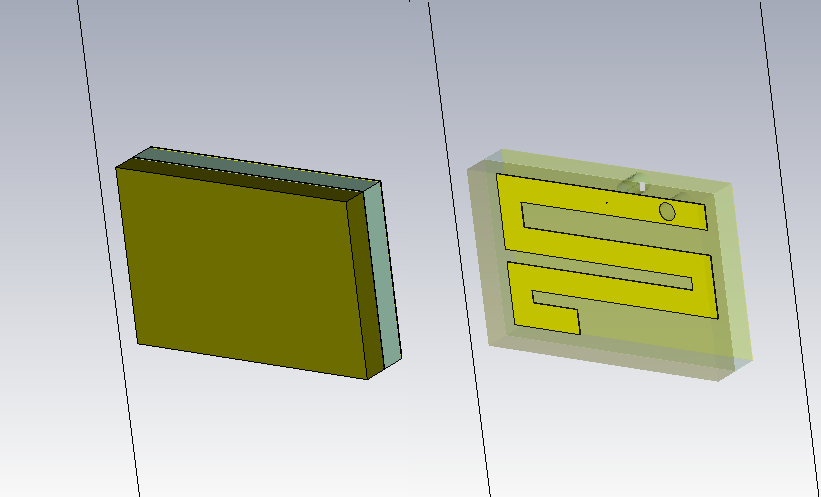
\includegraphics[scale=0.45]{./Simulaciones/original_antenna/original_antenna_copy}
    \caption{Diseño antena original construida en el software CST.}
    \label{fig:fig5.2}
\end{figure}

Al igual que en el artículo, por cada simulación que hagamos, realizaremos un estudio del parámetro $S_{11}$, del diagrama de radiación y de su campo eléctrico radiado. El parámetro $S_{11}$ nos informa sobre las frecuencias a las que la antena radia; el diagrama de radiación nos indicará hacia qué ángulo será más directiva la antena (donde mejor apunta y llega más potencia radiada) y el campo eléctrico nos dirá cómo está radiando la antena.

% S11 ANTENA SERPENTINA ORIGINAL SIN NADA
\begin{figure}[!htb]
    \centering
    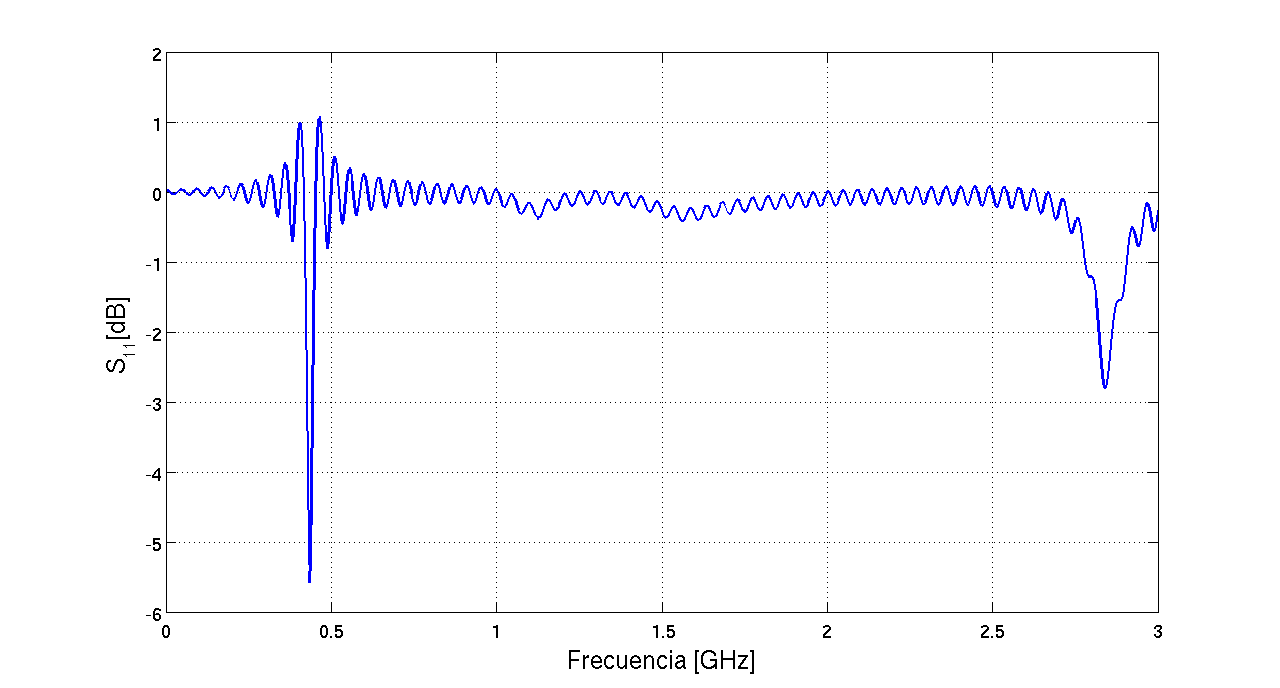
\includegraphics[scale=0.45]{./Simulaciones/matlab2/S11_original_free}
    \caption{Gráfica que recoge el parámetro $S_{11}$ de la antena de serpentina original en espacio libre.}
    \label{fig:fig5.3}
\end{figure}

En primer lugar, presentamos el resultado de la simulación del parámetro $S_{11}$. La \textit{fig. \ref{fig:fig5.3}} muestra que la antena del artículo simulada trabaja en un entorno muy parecido a la banda MICS, aunque en el espacio libre no llega a ser exactamente dicha banda. Las fluctuaciones que vemos en la gráfica se deben a la simulación realizada por el software CST. En comparación con el artículo, tenemos una variación importante, ya que según sus estudios, la banda central para la antena de serpentina en aire es de aproximadamente 370-380 MHz. En nuestro caso, la frecuencia de resonancia es de aproximadamente 435 MHz. Debemos decir que los autores del artículo no citan en ningún momento qué tipo de software han utilizado, por lo que la comparación realmente no llegará a ser exacta; lo único sí mencionado es que utilizan el método FDTD, utilizado también por nuestro software.\\

A continuación vamos a proceder a mostrar el campo eléctrico de la antena original. Para ello, se presentan cuatro figuras: las tres primeras, \textit{fig. \ref{fig:fig5.4}},~\textit{\ref{fig:fig5.5}} y~\textit{\ref{fig:fig5.6}}, son tres modelos en tres dimensiones de la antena y pequeños atributos que marcan la intensidad y dirección del campo; la última, \textit{fig. \ref{fig:fig5.7}} es una representación del campo en el parche radiante.

% E FIELD ANTENA SERPENTINA ORIGINAL SIN NADA
\begin{figure}[!htb]
    \centering
    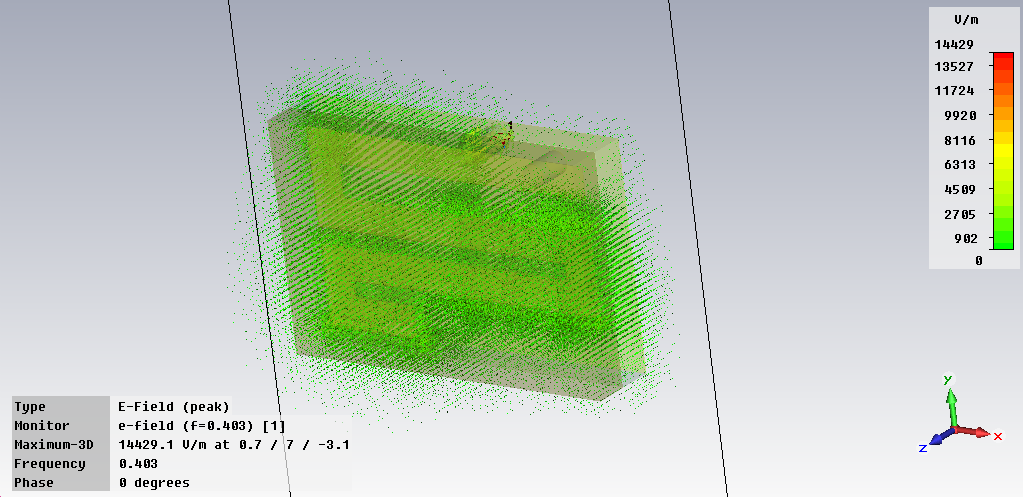
\includegraphics[scale=0.3]{./Simulaciones/original_antenna/original_antenna_E-Field}
    \caption{Representación del campo eléctrico en prespectiva.}
    \label{fig:fig5.4}
\end{figure}

\begin{figure}[!htb]
    \centering
    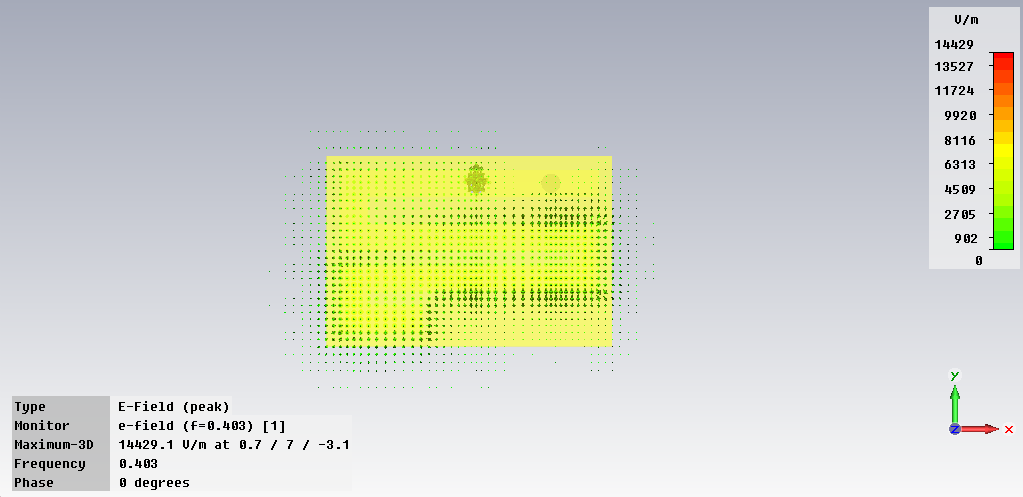
\includegraphics[scale=0.3]{./Simulaciones/original_antenna/original_antenna_E-Field_2}
    \caption{Representación del campo eléctrico desde el frente.}
    \label{fig:fig5.5}
\end{figure}

\begin{figure}[!htb]
    \centering
    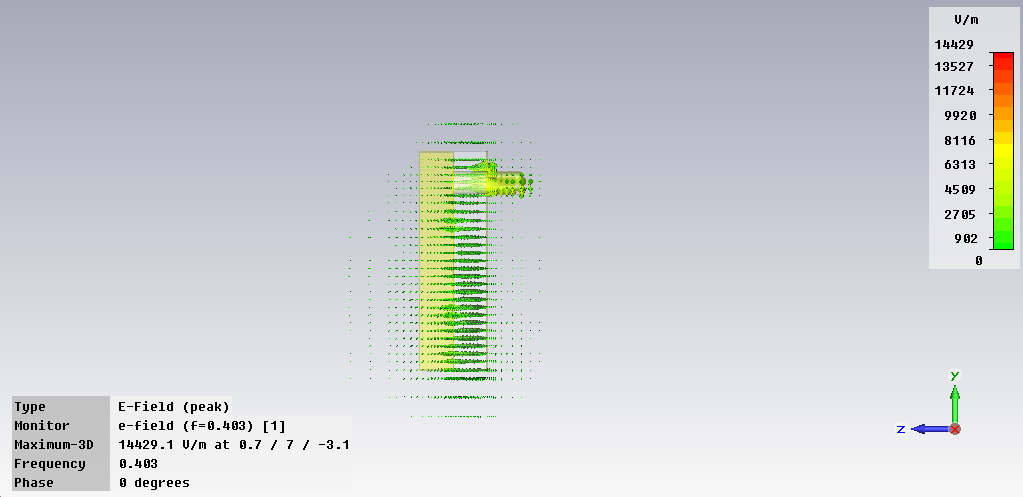
\includegraphics[scale=0.3]{./Simulaciones/original_antenna/original_antenna_E-Field_3}
    \caption{Representación del campo eléctrico desde el lado derecho.}
    \label{fig:fig5.6}
\end{figure}

\begin{figure}[!htb]
    \centering
    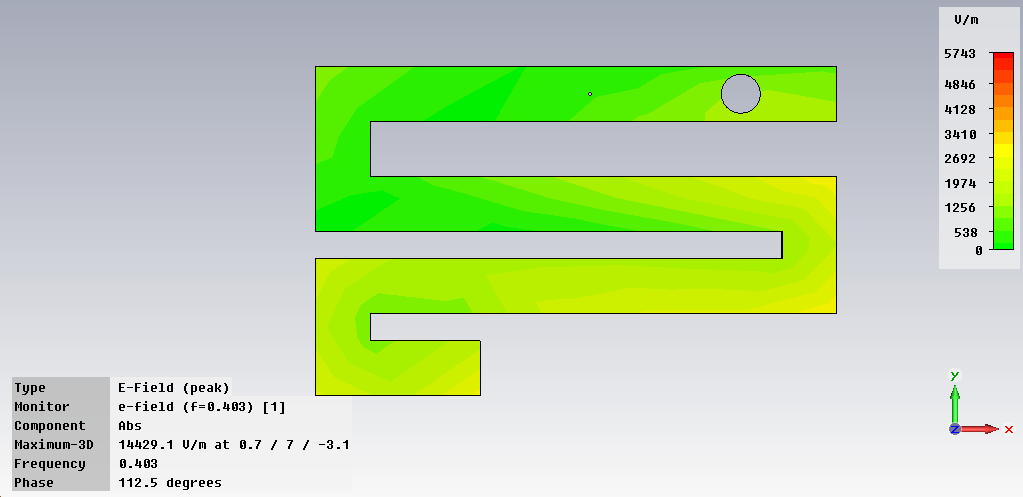
\includegraphics[scale=0.3]{./Simulaciones/original_antenna/original_antenna_E-Field_4}
    \caption{Representación del campo eléctrico justo en el parche radiante.}
    \label{fig:fig5.7}
\end{figure}

\clearpage

Como podemos ver, la antena radia campo eléctrico al exterior y sobre todo, si nos fijamos en las \textit{figs. \ref{fig:fig5.5}} y~\textit{\ref{fig:fig5.7}}, en la parte final de la serpentina. La representación del campo eléctrico en el artículo es muy parecida aunque no tenemos tanto detalles como en las imágenes anteriores.\\

Lo último que nos queda por ver es el diagrama de radiación. Tras la simulación encontramos que la antena es capaz de radiar con dos lóbulos principales tal y como podemos apreciar en la siguiente figura.

% DIAGRAMA DE RADIACION ANTENA SERPENTINA ORIGINAL SIN NADA
\begin{figure}[!htb]
    \centering
    \subfigure[]{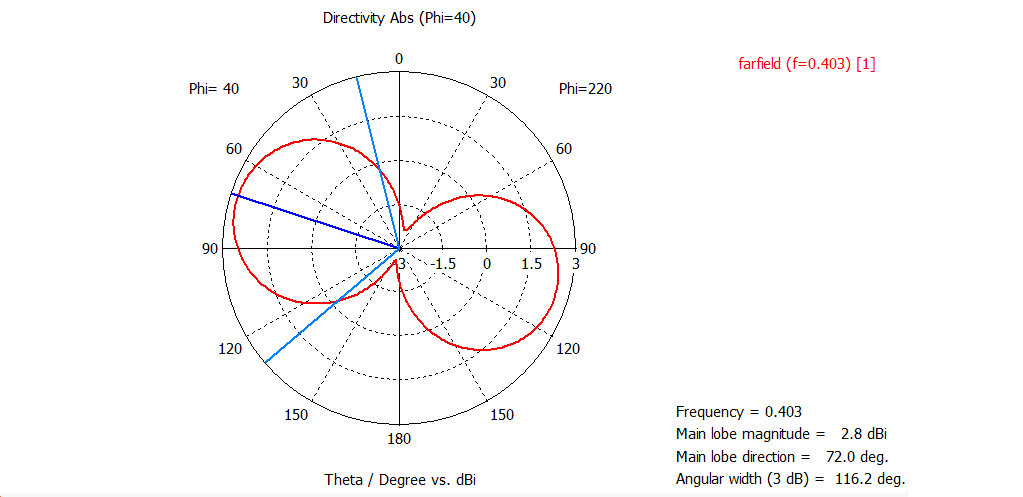
\includegraphics[scale=0.35]{./Simulaciones/original_antenna/original_antenna_radiation_pattern}}
    \subfigure[]{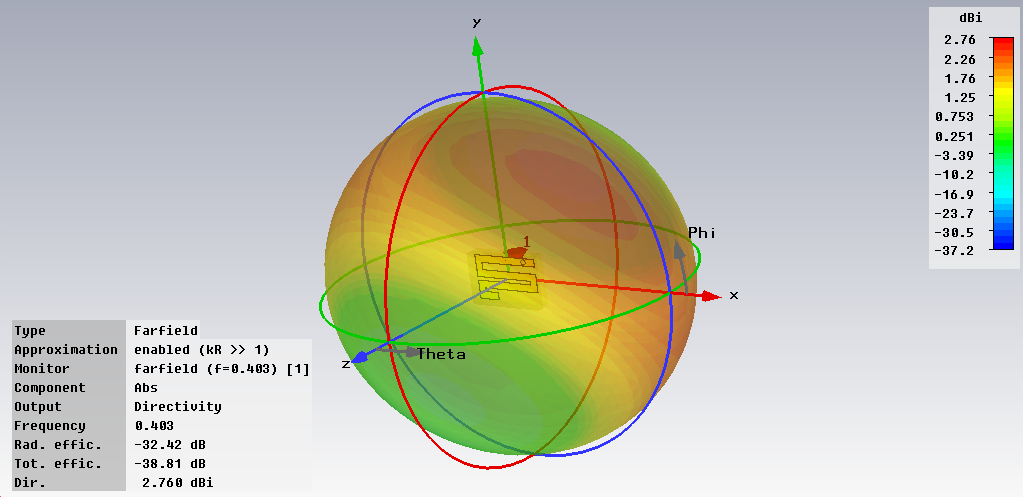
\includegraphics[scale=0.35]{./Simulaciones/original_antenna/original_antenna_radiation_pattern_3D}}
    \caption{Representación del diagrama de radiación de la antena original en espacio libre. En (a) coordenadas polares en 2D manteniendo $\phi$ = 40º y en (b) en 3D.}
    \label{fig:fig5.8}
\end{figure}

\clearpage

\subsection{Antena original rodeada de un bloque de músculo}\label{subsec:antena-original-rodeada-de-un-bloque-de-musculo}

Después de ver los distintos resultados de la antena original en espacio libre, procedemos a simular dicha antena dentro de un bloque de músculo. El diseño del artículo está pensado para esta opción, es decir, situar la antena dentro del cuerpo humano. En esta ocasión, hemos diseñado un bloque rectangular de músculo con el software CST en el cual hemos insertado la antena. Las propiedades dieléctricas del espacio cambian considerablemente, como podremos ver en las simulaciones.

Las propiedades del músculo construido son las siguientes:

% Tabla medidas músculo

\begin{table}[h]
    \centering\scalebox{0.99}{
        \begin{tabular}{| c | c | c | c | c | c |}
            \hline
            \textbf{Dimensiones}             & \textbf{mm} \\
            \hline
            \hline
            Largo                            & 50          \\
            \hline
            Alto                             & 40          \\
            \hline
            Ancho                            & 20          \\
            \hline
            \hline
            \textbf{Permitividad}            &             \\
            \textbf{relativa $\epsilon_{r}$} & 42.807      \\
            \hline
            \hline
            \textbf{Conductividad}           &             \\
            \textbf{eléctrica $\sigma$}      & 0.6463 S/m  \\
            \hline
            \hline
        \end{tabular}}
    \caption{Propiedades del bloque de músculo diseñado para su simulación.}
    \label{tab:tabla5.3}
\end{table}

En primer lugar, en la \textit{fig. \ref{fig:fig5.9}}, presentamos el diseño de la antena dentro del bloque de músculo. Como se aprecia en la imagen, lo único que cambia es el bloque rectangular que rodea la antena.

% ANTENA ORIGINAL EN MUSCULO
\begin{figure}[!htb]
    \centering
    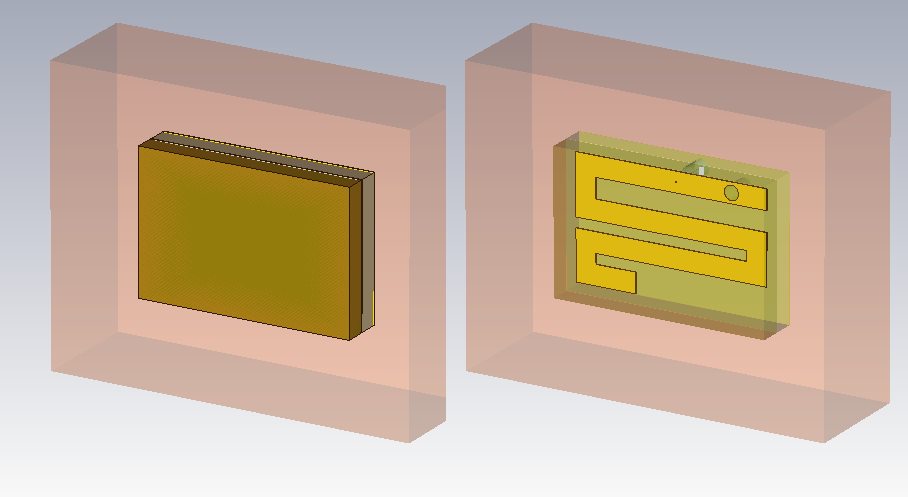
\includegraphics[scale=0.25]{./Simulaciones/original_antenna_muscle/original_serpentine_muscle_copy}
    \caption{Diseño antena original insertada en un bloque de músculo construida en el software CST.}
    \label{fig:fig5.9}
\end{figure}

\clearpage

La simulación del parámetro $S_{11}$ se recoge en la \textit{fig. \ref{fig:fig5.10}}.

% S11 ANTENA ORIGINAL EN MUSCULO
\begin{figure}[!htb]
    \centering
    \subfigure[]{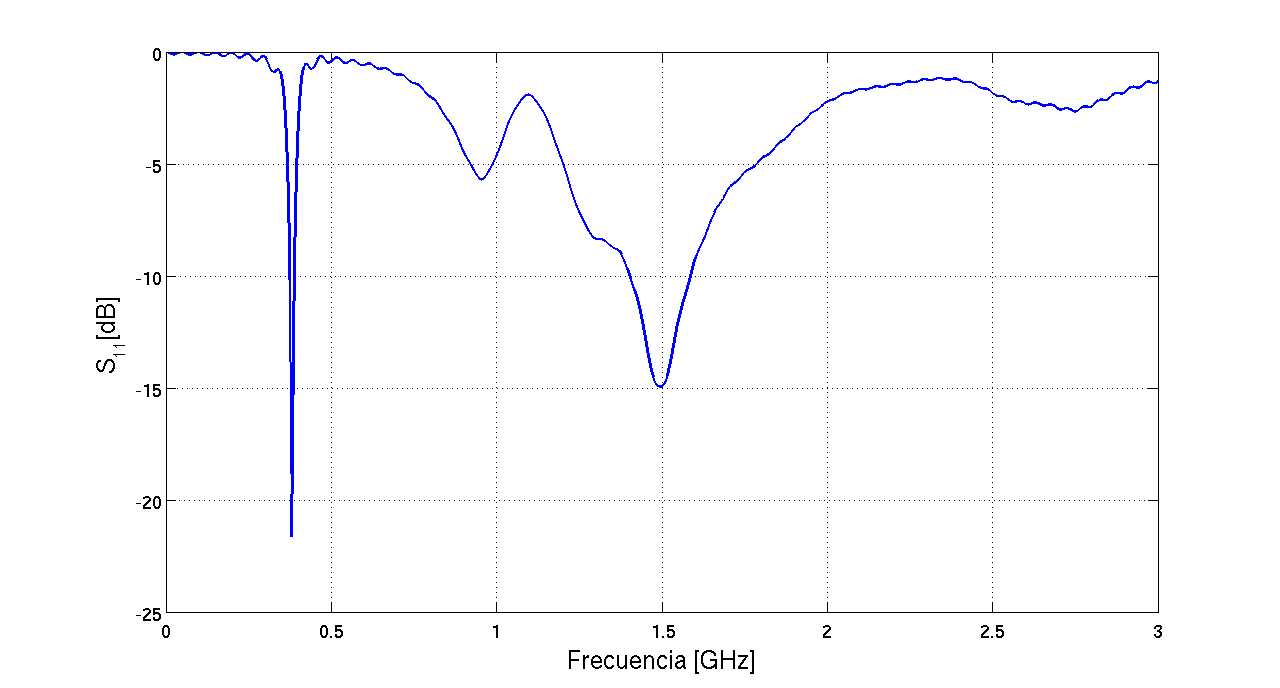
\includegraphics[scale=0.4]{./Simulaciones/matlab2/S11_original_muscle}}
    \subfigure[]{\includegraphics[scale=0.4]{./Simulaciones//matlab2/S11_original_muscle_zoom}}
    \caption{Gráficas que recogen el parámetro $S_{11}$ de la antena de serpentina original rodeada de músculo. En (a) medidas simuladas de 0 a 3 GHz y en (b) se ha aplicado un zoom en la banda MICS.}
    \label{fig:fig5.10}
\end{figure}

Las gráficas de la \textit{fig. \ref{fig:fig5.10}} dejan patente que la antena diseñada en el artículo permite trabajar en una banda cercana a la banda MICS, pero no exactamente en la misma banda. En el artículo, los autores proporcionan datos que sitúan esta antena simulada, en un entorno muy parecido o prácticamente igual en el que estamos trabajando, en una banda cercana a los 500 MHz, muy lejos de nuestra banda de trabajo. Sin embargo, nuestra simulación se acerca mucho más a la banda y como podemos apreciar en la gráfica zoom, \textit{fig. \ref{fig:fig5.10} (b)}, el mínimo $S_{11}$ está a escasos 20 MHz de la banda MICS, donde tenemos -3.02 dB de dicho parámetro. Por lo tanto, unas de las razones que nos empuja a seguir estudiando y considerando este diseño es centrar el mínimo valor de $S_{11}$ a la banda MICS. Como se anunció anteriormente, estas desigualdades entre el artículo y nuestra simulación son seguramente debidas a que no se usan el mismo software o quizá no estamos considerando algún parámetro extra que los autores no señalan.

Procedemos a ver el campo eléctrico de esta simulación, junto a la pérdida de potencia en el superestrato diélectrico de la antena y el diagrama de radiación.

%CAMPO ELÉCTRICO Y PÉRDIDA DE POTENCIA
\begin{figure}[!htb]
    \centering
    \includegraphics[scale=0.3]{./Simulaciones/original_antenna_muscle/original_serpentine_muscle_E-Field}
    \caption{Representación campo eléctrico en prespectiva.}
    \label{fig:fig5.11}
\end{figure}

\begin{figure}[!htb]
    \centering
    \includegraphics[scale=0.3]{./Simulaciones/original_antenna_muscle/original_serpentine_muscle_E-Field_2}
    \caption{Representación campo eléctrico desde el frente.}
    \label{fig:fig5.12}
\end{figure}

\begin{figure}[!htb]
    \centering
    \includegraphics[scale=0.3]{./Simulaciones/original_antenna_muscle/original_serpentine_muscle_E-Field_3}
    \caption{Representación campo eléctrico desde el lado derecho.}
    \label{fig:fig5.13}
\end{figure}

\begin{figure}[!htb]
    \centering
    \includegraphics[scale=0.3]{./Simulaciones/original_antenna_muscle/original_serpentine_muscle_E-Field_4}
    \caption{Representación campo eléctrico justo en el parche radiante.}
    \label{fig:fig5.14}
\end{figure}

\begin{figure}[!htb]
    \centering
    \includegraphics[scale=0.4]{./Simulaciones/original_antenna_muscle/original_serpentine_muscle_power_loss}
    \caption{Representación pérdida de potencia en el superestrato diélectrico.}
    \label{fig:fig5.15}
\end{figure}

\newpage

Las imágenes mostradas en las \textit{figs. \ref{fig:fig5.11}},~\textit{\ref{fig:fig5.12}},~\textit{\ref{fig:fig5.13}} y~\textit{\ref{fig:fig5.14}}, reflejan cómo el campo eléctrico se distribuye alrededor de la antena, enfatizando la densidad del mismo en la región inferior. En la \textit{fig. \ref{fig:fig5.14}} se puede ver cómo ha aumentado el campo eléctrico radiado a través del parche en comparación a exponer la antena al espacio libre, \textit{fig. \ref{fig:fig5.7}}. La misma comparación es observada en las distintas figuras representadas en tres dimensiones, demostrando que la antena es más efectiva en un medio dieléctrico como el músculo que en el espacio libre.

La imagen representada en \textit{fig. \ref{fig:fig5.15}} muestra la pérdida de potencia en el superstrato dieléctrico. Nos indica concretamente en qué zonas radia la antena al exterior y por dónde se está perdiendo eficiencia en cuanto a la potencia total entregada a la propia antena.

El diagrama de radiación de la antena rodeada de músculo queda de la siguiente manera:

\begin{figure}[!htb]
    \centering
    \subfigure[]{\includegraphics[scale=0.3]{./Simulaciones/original_antenna_muscle/original_serpentine_muscle_radiation_pattern}}
    \subfigure[]{\includegraphics[scale=0.3]{./Simulaciones/original_antenna_muscle/original_serpentine_muscle_radiation_pattern_3D}}
    \caption{Representación del diagrama de radiación de la antena original en tejido muscular. En (a) coordenadas polares en 2D manteniendo $\phi$ = 85º y en (b) en 3D.}
    \label{fig:fig5.16}
\end{figure}

Ha habido un cambio notable frente al diagrama de radiación de la antena en espacio libre: ya no existen dos lóbulos principales bien diferenciados. En su lugar, el lóbulo principal se ha situado en 60º $\theta$ aproximadamente, dejando fijo $\phi$ a 85º, y el lóbulo posterior se ha visto reducido. Además la antena radia hacia el frente con valor de ganancia 3.3 dBi, alto con respecto a la eficiencia pérdida por potencia.
En esta última figura se ve claramente la zona roja, de máxima radiación, situada en una zona superior a la antena, como bien dice el diagrama de radiación en coordenadas polares, a 60º aproximadamente de la normal de la antena.\\

Hemos comprobado mediante simulación realizada por sofrware de computadora cómo funciona la antena del artículo de Soontorpipit. Según nuestras simulaciones, esta antena puede ser expuesta a muchas modificaciones para su correcto funcionamiento en la banda MICS e incluso mejorar su eficiencia en dicha banda. A continuación, vamos a tomar esta antena como referencia y modificar ciertos parámetros que incluso los autores proponen como mejora en sus conclusiones.


\section{Estudio paramétrico de la antena de serpentina propuesta}\label{sec:modificado}

La idea que hemos dejado plasmada en el anterior párrafo la debemos llevar a cabo modificando en primer lugar las dimensiones del parche radiante, la estructura de serpentina en sí. Como sabemos del artículo, existen tres medidas catalogadas por los autores como B, C y D. Dichas medidas corresponden con la longitud del último brazo, la distancia entre el pin de tierra y el pin de alimentación y la distancia entre el principio de la estructura y el pin de tierra respectivamente. Originalmente, las medidas son: \textbf{B = 8.4 mm, C = 7.7 mm y D = 4.9 mm}.

Los estudios que se han realizado en simulación de una posible antena modificada quedan reflejados en la siguiente tabla, donde se expone qué se ha cambiado y qué resultados se han obtenido. Los materiales son los mismos con los que se ha simulado la antena original, únicamente se ha modificado las dimensiones del parche radiante. Huelga decir que se ha intentado desde el primer momento tanto mejorar el parámetro $S_{11}$ como centrar la frecuencia de resonancia a la banda MICS; además, todas las simulaciones para encontrar el diseño definitivo se han hecho con la antena rodeada de un bloque de músculo.

% TABLA DIFERENTES RESULTADOS

\begin{table}[h]
    \centering\scalebox{0.85}{
        \begin{tabular}{| c | c | c | c | c | c |}
            \hline
            %\fcolorbox{orange}{orange}{ \color{white} LaTeX}
            \textbf{Parámetro modificado} & \textbf{Frecuencia de resonancia} & \textbf{Parámetro $S_{11}$} & \textbf{Ganancia} \\
            \hline
            \hline
            B = 5 mm                      & 393 MHz                           & -26.27 dB                   & 2.8 dBi                           \\
            \hline
            B = 4.5 mm                    & 393 MHz                           & -32.65 dB                   & 2.6 dBi                           \\
            \hline
            B = 4.5 mm                    &                                   &                             &                                   \\
            D = 6 mm                      & 402 MHz                           & -25.27 dB                   & 2.6 dBi                           \\
            \hline
            B = 4.5 mm                    &                                   &                             &                                   \\
            D = 7 mm                      & 408 MHz                           & -25.78 dB                   & 2.6 dBi                           \\
            \hline
            B = 4.5 mm                    &                                   &                             &                                   \\
            D = 6.5 mm                    & 402 MHz                           & -25.43 dB                   & 2.6 dBi                           \\
            \hline
            B = 4.5 mm                    &                                   &                             &                                   \\
            C = 7.8 mm                    & 402 MHz                           & -25.87 dB                   & 2.6 dBi                           \\
            D = 6.5 mm                    &                                   &                             &                                   \\
            \hline
            \textbf{B = 6 mm}             &                                   &                             &                                   \\
            \textbf{C = 7.8 mm}           & \textbf{402 MHz}                  & \textbf{-41.7 dB}           & \textbf{2.7 dBi ($\theta$ = 85º)} \\
            \textbf{D = 7 mm}             &                                   &                             &                                   \\
            \hline
            \hline
        \end{tabular}}
    \caption{Pruebas realizadas para modificar el diseño original de la antena de serpentina.}
    \label{tab:tabla5.4}
\end{table}

En esta tabla, podemos ver las distintas modificaciones que se han realizado al parche de serpentina hasta conseguir unos valores óptimos con un parámetro $S_{11}$ de -41.7 dB a 402 MHz. Los parámetros de ancho y largo de los substratos tampoco se han visto modificados. Vamos a proceder a simular la antena con las últimas características, \textbf{B = 6 mm, C = 7.8 mm, D = 7 mm}, tanto en espacio libre como en músculo. Añadiremos un tercer punto de estudio con una estructura de tres capas, piel, grasa y músculo, intentando simular lo máximo posible un entorno real.

\subsection{Antena modificada en espacio libre}\label{subsec:antena-modificada-en-espacio-libre}

En nuestro software CST para modificar la antena origianl únicamente tenemos que cambiar los parámetros globales que tenemos definidos como B, C y D. Tras cambiar las variables, el diseño se actualiza automáticamente, presentando un nuevo aspecto como se ve en la \textit{fig. \ref{fig:fig5.17}}. Quizá no se aprecia bien los cambios, pero hemos de recordar que modificamos milímetros, apenas apreciables a simple vista; no obstante si se compara con el diseño anterior se ve que el último brazo se ha reducido y la distancia entre pines también ha cambiado.

% ANTENA MODIFICADA
\begin{figure}[!htb]
    \centering
    \subfigure[]{\includegraphics[scale=0.35]{./Simulaciones/tunned_antenna/tunned_serpentine_antenna}}
    \subfigure[]{\includegraphics[scale=0.35]{./Simulaciones/tunned_antenna/antenna_comparacion}}
    \caption{Antena microstrip en forma de serpentina modificada. En (a) el diseño completo y en (b) comparación entre la antena original (izquierda) y la modificada (derecha).}
    \label{fig:fig5.17}
\end{figure}

El parámetro $S_{11}$ en este caso, simulación en espacio libre, tiene una forma similar al que presentamos en la sección anterior, con sus impulsos debidos al software y su frecuencia desviada. Incluso en esta ocasión, su frecuencia de resonancia es más alta, como se ven en la \textit{fig. \ref{fig:fig5.19}}, debido seguramente a que hemos acortado la longitud del parche radiante, que es el que fundamentalmente marca dicha frecuencia. En definitiva, pasamos de tener una frecuencia de resonancia de 435 MHz a 456 MHz.

% S11 ANTENA MODIFICADA
\begin{figure}[!htb]
    \centering
    \includegraphics[scale=0.45]{./Simulaciones/matlab2/S11_tunned_free}
    \caption{Gráfica que recoge el parámetro $S_{11}$ de la antena de serpentina modificada en espacio libre.}
    \label{fig:fig5.18}
\end{figure}

\begin{figure}[!htb]
    \centering
    \includegraphics[scale=0.45]{./Simulaciones/matlab2/S11_vs_original_tunned_free_zoom}
    \caption{Gráfica zoom que recoge el parámetro $S_{11}$ de las antenas original y modificada en espacio libre.}
    \label{fig:fig5.19}
\end{figure}

\clearpage

El campo eléctrico para nuestra antena modificada en espacio libre queda muy similar a la antena original. En la \textit{fig. \ref{fig:fig5.20}} se exponen cuatro imágenes del resultado.

% E FIELD ANTENA MODIFICADA
\begin{figure}[!htb]
    \centering
    \subfigure[]{\includegraphics[scale=0.25]{./Simulaciones/tunned_antenna/tunned_serpentine_antenna_E-Field}}
    \subfigure[]{\includegraphics[scale=0.25]{./Simulaciones/tunned_antenna/tunned_serpentine_antenna_E-Field_2}}
    \subfigure[]{\includegraphics[scale=0.25]{./Simulaciones/tunned_antenna/tunned_serpentine_antenna_E-Field_3}}
    \subfigure[]{\includegraphics[scale=0.25]{./Simulaciones/tunned_antenna/tunned_serpentine_antenna_E-Field_4}}
    \caption{Representación del campo eléctrico de la antena modificada en espacio libre. En (a) vista en prespectiva; en (b) vista frontal; en (c) vista desde el lado derecho y en (d) vista del parche radiante.}
    \label{fig:fig5.20}
\end{figure}

Como venimos haciendo hasta ahora, representamos además el diagrama de radiación correspondiente. Éste ha cambiado respecto al original del artículo, ya que los lóbulos han modificado su posición y se encuentran en otra ángulo $\theta$ respecto a $\phi$, fijado en aproximadamente 215º. Sin embargo, el propio software de CST nos indica que este diseño no es adecuado, ya que la radiación efectiva es muy baja, es decir, nuestra antena modificada para espacio libre radia muy poco campo al exterior. Los resultados tanto en coordenadas polares como en 3D podemos verlos en la \textit{fig. \ref{fig:fig5.21}}.

% DIAGRAMA DE RADIACION ANTENA MODIFICADA
\begin{figure}[!htb]
    \centering
    \subfigure[]{\includegraphics[scale=0.6]{./Simulaciones/tunned_antenna/tunned_serpentine_antenna_radiation_pattern}}
    \subfigure[]{\includegraphics[scale=0.6]{./Simulaciones/tunned_antenna/tunned_serpentine_antenna_radiation_pattern_3D}}
    \caption{Representación del diagrama de radiación de la antena modificada en espacio libre. En (a) coordenadas polares en 2D manteniendo $\phi$ = 215º y en (b) en 3D, donde podemos ver la advertencia del programa en cuanto a la radiación efectiva.}
    \label{fig:fig5.21}
\end{figure}

\clearpage

\subsection{Antena modificada rodeada de músculo}\label{subsec:antena-modificada-rodeada-de-musculo}

Esta sección es importante ya que veremos si nuestro diseño modificado a partir del propuesto en el artículo ofrece mejores resultados con las condiciones de simulación que tenemos. La única novedad respecto a la sección anterior es que rodeamos nuestra antena de un bloque de músculo.

% ANTENA MODIFICADA MUSCULO
\begin{figure}[!htb]
    \centering
    \includegraphics[scale=0.45]{./Simulaciones/tunned_antenna_muscle/tunned_serpentine_muscle}
    \caption{Diseño de la antena modificada rodeada de un bloque de músculo.}
    \label{fig:fig5.22}
\end{figure}

Los resultados del parámetro $S_{11}$ mejoran a los simulados anteriormente en la misma condición con bloque de músculo. Se obtiene un valor de -41.7 dB en la banda MICS tal y como se aprecia en la \textit{fig. \ref{fig:fig5.23}}. El dato es muy positivo para nuestro proyecto y para nuestro conjunto de simulaciones.

% S11 ANTENA MODIFICADA MUSCULO
\begin{figure}[!htb]
    \centering
    \subfigure[]{\includegraphics[scale=0.45]{./Simulaciones/matlab2/S11_tunned_muscle}}
    \subfigure[]{\includegraphics[scale=0.45]{./Simulaciones/matlab2/S11_tunned_muscle_zoom}}
    \caption{Gráficas que recogen el parámetro $S_{11}$ de la antena de serpentina modificada en tejido muscular. En (a) medidas simuladas de 0 a 3 GHz y en (b) se ha aplicado un zoom en la banda MICS.}
    \label{fig:fig5.23}
\end{figure}

El valor de -41.7 dB es mejor que el anterior dato obtenido en el mismo entorno de simulación (-3.02 dB en la banda MICS). Nos indica que nuestra antena modificada supera en el parámetro $S_{11}$ a la antena que hemos simulado a partir del artículo. Uno de los inconvenientes encontrados es el reducido ancho de banda, debido al grosor del substrato, pero tampoco podemos aumentarlo más, porque perderíamos eficiencia en radiación. Otra desventaja importante es en el caso de construir la antena de manera fisica: será muy difícil conseguir estos valores, seguramente nos lo impidan el uso de la conexión directa por cable coaxial o por algún fallo o error en la construcción de la antena, es decir, impurezas al cortar los materiales o imperfecciones de los mismos.

\clearpage

En comparación con la simulación obtenida con la antena original en músculo, tenemos mejor valor de $S_{11}$ y una frecuencia centrada en la banda MICS.

\begin{figure}[!htb]
    \centering
    \subfigure[]{\includegraphics[scale=0.4]{./Simulaciones/matlab2/S11_vs_original_tunned_muscle}}
    \subfigure[]{\includegraphics[scale=0.4]{./Simulaciones/matlab2/S11_vs_original_tunned_muscle_zoom}}
    \caption{Comparación parámetro $S_{11}$ de la antena original y la modificada en músculo. En (a) barrido de frecuencias de 0 a 3 GHz y en (b) zoom en la banda MICS.}
    \label{fig:fig5.24}
\end{figure}

\clearpage

A continuación, mostraremos el campo eléctrico de nuestra antena modificada en las \textit{figs. \ref{fig:fig5.25}},~\textit{\ref{fig:fig5.26}},~\textit{\ref{fig:fig5.27}} y~\textit{\ref{fig:fig5.28}}.

% E FIELD ANTENA MODIFICADA MUSCULO
\begin{figure}[!htb]
    \centering
    \includegraphics[scale=0.4]{./Simulaciones/tunned_antenna_muscle/tunned_serpentine_muscle_E-Field}
    \caption{Representación campo eléctrico en prespectiva.}
    \label{fig:fig5.25}
\end{figure}

\begin{figure}[!htb]
    \centering
    \includegraphics[scale=0.4]{./Simulaciones/tunned_antenna_muscle/tunned_serpentine_muscle_E-Field_2}
    \caption{Representación campo eléctrico desde el frente.}
    \label{fig:fig5.26}
\end{figure}

\begin{figure}[!htb]
    \centering
    \includegraphics[scale=0.4]{./Simulaciones/tunned_antenna_muscle/tunned_serpentine_muscle_E-Field_3}
    \caption{Representación campo eléctrico desde el lado derecho.}
    \label{fig:fig5.27}
\end{figure}

\begin{figure}[!htb]
    \centering
    \includegraphics[scale=0.4]{./Simulaciones/tunned_antenna_muscle/tunned_serpentine_muscle_E-Field_4}
    \caption{Representación campo eléctrico en el parche radiante.}
    \label{fig:fig5.28}
\end{figure}

En las \textit{figs. \ref{fig:fig5.25}},~\textit{\ref{fig:fig5.26}},~\textit{\ref{fig:fig5.27}} y~\textit{\ref{fig:fig5.28}} anteriores hemos podido comprobar cómo se distribuye el campo en la antena. Sucede al igual que antes, la mayoría del campo eléctrico se dispone en la parte baja del parche y sale al exterior así, generando los \textit{fringing fields} u ondas viajeras, que son las que hacen que una antena funcione y radie. La posición del pin de tierra junto al de alimentación son clave para conseguir la frecuencia de resonancia a la que trabajamos y conseguir estos campos.

La distribución de pérdida de potencia se muestra en la \textit{fig. \ref{fig:fig5.29}}.

% PÉRDIDA DE POTENCIA ANTENA MODIFICADA MÚSCULO
\begin{figure}[!htb]
    \centering
    \includegraphics[scale=0.5]{./Simulaciones/tunned_antenna_muscle/tunned_serpentine_muscle_power_loss}
    \caption{Representación de la pérdida de potencia en el dieléctrico.}
    \label{fig:fig5.29}
\end{figure}

Al igual que sucedía con la antena original, la potencia se pierde por los lados más bajos del dieléctrico. Quizá esto pueda ser también un punto de estudio para conseguir una antena que consiga una eficiencia energética mayor, sin tener muchas pérdidas por ondas reflejadas u ondas superficiales.

El diagrama de radiación de nuestra antena modificada resulta muy parecido al de la antena original. Sin embargo, hemos perdido ganancia en la antena, seguramente debido a la disminución del parámetro $S_{11}$. Otro punto de estudio interesante sería conseguir un compromiso entre la ganancia de la antena y el parámetro $S_{11}$.

% DIAGRAMA DE RADIACIÓN ANTENA MODIFICADA MÚSCULO
\begin{figure}[!htb]
    \centering
    \subfigure[]{\includegraphics[scale=0.5]{./Simulaciones/tunned_antenna_muscle/tunned_serpentine_muscle_radiation_pattern}}
    \subfigure[]{\includegraphics[scale=0.5]{./Simulaciones/tunned_antenna_muscle/tunned_serpentine_muscle_radiation_pattern_3D}}
    \caption{Representación del diagrama de radiación de la antena modificada en tejido muscular. En (a) coordenadas polares en 2D manteniendo $\phi$ = 85º y en (b) en 3D.}
    \label{fig:fig5.30}
\end{figure}

El lóbulo principal se establece a unos 60º $\theta$, recayendo toda la radiación hacia la parte superior de la antena, como podemos apreciar en la imagen en 3D \textit{fig. \ref{fig:fig5.30} (b)}: la zona roja. En definitiva, se ha conseguido un ancho de haz de 120º. Una simulación posterior a esta podría ser comprobar la corriente superficial en el parche en dos antenas iguales a nuestra antena modificada: una haciendo de transmisor y otra de receptor, para comprobar el \textit{teorema de reciprocidad} con esta antena, el cual establece que cualquier dispositivo que radie potencia en forma de ondas electromagnéticas, una antena en términos coloquiales, funciona igualmente como transmisor y como receptor.

\subsection{Antena modificada rodeada de tres capas de tejido: piel, grasa y músculo}\label{subsec:3capas}

Nuestra antena modificada parece eficiente según estas simulaciones mostradas anteriormente. Ahora bien, ¿y si simulamos nuestra antena en un entorno más real?, es decir, ¿con más tejidos corporales? El artículo de referencia hace experimentos además de con músculo, con otros tipos de tejidos. En nuestro caso, con la antena modificada, vamos a simular en un entorno más realista: colocaremos la antena en un entorno electromagnético consistente en tres capas, piel, grasa y músculo. Podemos ver este diseño en la \textit{fig. \ref{fig:fig5.31}}.

% ANTENA MODIFICADA 3 CAPAS
\begin{figure}[!htb]
    \centering
    \subfigure[]{\includegraphics[scale=0.5]{./Simulaciones/tunned_antenna_3layers/tunned_serpentine_3layers}}
    \subfigure[]{\includegraphics[scale=0.5]{./Simulaciones/tunned_antenna_3layers/tunned_serpentine_3layers_2}}
    \caption{Representación de la antena modificada en el entorno dieléctrico de tres capas: piel, grasa y músculo. En (a) vista general con orden de capas desde el frente hacia atrás: piel, grasa y músculo. En (b) vista de la antena introducida entre las tres capas.}
    \label{fig:fig5.31}
\end{figure}

% TABLA CONB MEDIDAS BLOQUE DE TRES CAPAS

Las medidas y carcaterísticas de los materiales del bloque diseñado de tres capas se recogen en la tabla siguiente:

% Tabla medidas bloque 3 capas
% Piel. Largo = 50 mm,alto = 40 mm,ancho = 14 mm, E_r = 31.29, Conductividad = 8.0138 S/m
% Grasa. Largo = 50 mm,alto = 40 mm,ancho = 3 mm, E_r = 4.6023, Conductividad = 0.58521 S/m
% Músculo. Largo 50 mm= ,alto = 40 mm,ancho = 6 mm, E_r = 42.807, Conductividad = 0.6463 S/m

\begin{table}[h]
    \centering\scalebox{0.99}{
        \begin{tabular}{| c | c | c | c | c | c |}
            \hline
            \textbf{Material} & \textbf{Dimensiones} & \textbf{Permitividad} & \textbf{Conductividad}   \\
            & \textbf{[mm]}        & \textbf{relativa}     & \textbf{eléctrica [S/m]} \\
            \hline
            \hline
            \textbf{Piel}     & 50 x 40 x 14         & 31.29                 & 8.0138                   \\
            \hline
            \hline
            \textbf{Grasa}    & 50 x 40 x 3          & 4.6023                & 0.58521                  \\
            \hline
            \hline
            \textbf{Músculo}  & 50 x 40 x 6          & 42.807                & 0.6463                   \\
            \hline
            \hline
        \end{tabular}}
    \caption{Propiedades del bloque de tres capas (piel, grasa y músculo) diseñado para la simulación.}
    \label{tab:tabla5.5}
\end{table}

En cuanto al parámetro $S_{11}$, de nuevo ha sido modificado y no está centrado en la banda MICS, aunque tiene buenas propiedades para ella. Por supuesto, ha influido el nuevo entorno dieléctrico en el que nos encontramos, ya no es una única permitividad relativa $\epsilon_{r}$: ahora hay tres y muy distintas todas ellas. Dicho desplazamiento podemos verlo en las \textit{figs. \ref{fig:fig5.32} (a)} y \textit{(b)}.

% S11 ANTENA MODIFICADA 3 CAPAS
\begin{figure}[!htb]
    \centering
    \subfigure[]{\includegraphics[scale=0.45]{./Simulaciones/matlab2/S11_tunned_3layers}}
    \subfigure[]{\includegraphics[scale=0.45]{./Simulaciones/matlab2/S11_tunned_3layers_zoom}}
    \caption{Gráficas que recogen el parámetro $S_{11}$ de la antena modificada en de tres capas. En (a) medidas simuladas de 0 a 3 GHz y en (b) se ha aplicado un zoom en la banda MICS.}
    \label{fig:fig5.32}
\end{figure}

Para la banda MICS, tenemos -7.74 dB $\simeq$ -8 dB, lo cual está razonablemente bien para un simulación que asemeja un entorno real. Un punto de estudio también interesante sería modificar esta antena, a partir de la que tenemos, para que trabaje perfectamente en la banda MICS.

\clearpage

En comparación con la simulación en músculo, nuestro mínimo $S_{11}$ se desplaza a una frecuencia menor, 393 MHz: representado en \textit{figs. \ref{fig:fig5.32} (b)} y~\textit{\ref{fig:fig5.33}}.

\begin{figure}[!htb]
    \centering
    \includegraphics[scale=0.45]{./Simulaciones/matlab2/S11_vs_tunned_3layers_muscle_zoom}
    \caption{Gráfica comparativa del parámetro $S_{11}$ entre la antena modificada simulada en músculo y con tres capas de tejido.}
    \label{fig:fig5.33}
\end{figure}

La posible razón del desplazamiento sufrido es debido al cambio de entorno dieléctrico. En la anterior simulación, la antena está rodeada completamente de tejido muscular y en esta ocasión, la antena está rodeada en su mayoría por el tejido de piel. Aún así, es razonable pensar que la antena funcionaría mejor en la banda MICS si se corrigieran estos defectos, modificando el parche radiante o los materiales.\\

El campo eléctrico radiado en esta situación nos lo muestra la \textit{fig. \ref{fig:fig5.34}}. No ha habido grandes cambios con respecto a las simulaciones anteriores, pero se asemejan mucho más a las simulaciones en tejido muscular que en espacio libre.

% E FIELD ANTENA MODIFICADA 3 CAPAS
\begin{figure}[!htb]
    \centering
    \subfigure[]{\includegraphics[scale=0.32]{./Simulaciones/tunned_antenna_3layers/tunned_serpentine_3layers_E-Field}}
    \subfigure[]{\includegraphics[scale=0.32]{./Simulaciones/tunned_antenna_3layers/tunned_serpentine_3layers_E-Field_2}}
    \subfigure[]{\includegraphics[scale=0.32]{./Simulaciones/tunned_antenna_3layers/tunned_serpentine_3layers_E-Field_3}}
    \subfigure[]{\includegraphics[scale=0.32]{./Simulaciones/tunned_antenna_3layers/tunned_serpentine_3layers_E-Field_4}}
    \caption{Representación del campo eléctrico en distintas vistas para la antena modificada en el entorno de tres capas. En (a) vista en prespectiva; en (b) vista frontal; en (c) vista desde el lado derecho y en (d) vista del parche radiante.}
    \label{fig:fig5.34}
\end{figure}

\clearpage

El diagrama de radiación de este modelo se ve en la \textit{fig. \ref{fig:fig5.35}}:

% DIAGRAMA DE RADIACIÓN ANTENA MODIFICADA 3 CAPAS
\begin{figure}[!htb]
    \centering
    \subfigure[]{\includegraphics[scale=0.4]{./Simulaciones/tunned_antenna_3layers/tunned_serpentine_3layers_radiation_pattern}}
    \subfigure[]{\includegraphics[scale=0.4]{./Simulaciones/tunned_antenna_3layers/tunned_serpentine_3layers_radiation_pattern_3D}}
    \caption{Representación del diagrama de radiación de la antena modificada en tejido muscular. En (a) coordenadas polares en 2D manteniendo $\phi$ = 90º y en (b) en 3D, donde podemos ver la advertencia del programa en cuanto a la radiación efectiva.}
    \label{fig:fig5.35}
\end{figure}

Las imágenes nos muestran dos lóbulos, el principal y el posterior muy similares a los vistos en tejido muscular. El ancho de haz a 3 dB en este caso es un poco mayor, pero lo encontramos a los mismos 60º $\theta$.

Como podemos comprobar, la radiación efectiva es muy pobre, está por debajo de los -40 dB, por lo que el diseño de la antena ha de ser modificado bastante más si queremos que funcione a la perfección dentro de un entorno de piel, grasa y músculo. Únicamente se ha modificado como se vió en la sección anterior los parámetros del parche, las medidas \textit{B, C} y \textit{D}; por consiguiente, ha de modificarse y estudiarse otros parámetros como las propias medidas de la antena o el grosor de los capas dieléctricas o los materiales, etc. Para simplificar nuestro proyecto y por diversas limitaciones que mencionaremos más adelante, se ha buscado eficiencia exclusivamente en entornos con tejido muscular.

Al igual que venimos diciendo a lo largo de este capítulo, hay diversos puntos de estudio que se pueden engrosar dentro de una serie de líneas futuras de trabajo a partir del estudio plasmado en estas hojas. Basándonos en nuestro diseño modificado se puede por ejemplo, mejorar la eficiencia de la antena, otros tipos de conectores, mejorar las prestaciones para entornos multicapa, etc.


\section{Diseño optimizado de la antena de serpentina propuesta con nuevos materiales}\label{sec:optimizado}

En este apartado vamos a buscar la eficiencia de nuestra antena con nuevos materiales. El motivo de los nuevos materiales tiene su razón en que son materiales muy utilizados y muy habituales en laboratorios que fabrican dispositivos eléctricos. Son además materiales que poseen características parecidas a los materiales propuestos en el artículo. Los materiales originales dieléctricos, \textit{Macor} y \textit{Alumina}, han sido sustituidos por los recogidos en la \textit{tabla \ref{tab:tabla5.6}}:

% Tabla con materiales nuevos

\begin{table}[h]
    \centering\scalebox{0.99}{
        \begin{tabular}{| c | c | c | c | c | c |}
            \hline
            \textbf{Materiales dieléctricos}           & \textbf{$\epsilon_{r}$} & Grosor [mm] \\
            \hline
            \hline
            Arlon 1000 (substrato)                     & 10                      & 2.54        \\
            \hline
            Policloruro de vinilo (PVC) (superestrato) & 3.19                    & 3           \\
            \hline
            \hline
            \textbf{Parche, masa y conectores}         & \textbf{$\sigma$ [S/m]} & Grosor [mm] \\
            \hline
            \hline
            Cobre                                      & 5.8 · $10^7$            & 0.1         \\
            \hline
            \hline
        \end{tabular}}
    \caption{Materiales nuevos para la antena de serpentina adaptada del artículo de Soontornpipit.}
    \label{tab:tabla5.6}
\end{table}

Como podemos observar en la \textit{tabla \ref{tab:tabla5.6}}, se ha modificado el grosor de la capa del substrato, que pasa de 3 mm a 2.54 mm. Este cambio sucede porque los materiales disponibles en laboratorios vienen de fábrica con unos espesores fijos y en el caso de \textit{Arlon 1000}, este espesor es de 1.27 mm. Al poner dos capas de este material, hemos obtenido un grosor de 2.54 mm, un valor cercano a los 3 mm originales.

Al igual que sucede en la anterior sección con el diseño modificado, aquí también debemos rediseñar las dimensiones del parche radiante. Cabe indicar que las dimensiones de la antena son idénticas de nuevo, por lo que lo único que se va a modificar son las dimensiones del parche y el grosor de la capa del substrato. La \textit{tabla \ref{tab:tabla5.7}} recoge los parámetros que han sido cambiados y la evolución hasta conseguir un parámetro $S_{11}$ eficiente.

\begin{table}[h]
    \centering\scalebox{0.85}{
        \begin{tabular}{| c | c | c | c | c | c |}
            \hline
            %\fcolorbox{orange}{orange}{ \color{white} LaTeX}
            \textbf{Parámetro modificado} & \textbf{Frecuencia de resonancia} & \textbf{Parámetro $S_{11}$} & \textbf{Ganancia} \\
            \hline
            \hline
            B = 6 mm                      &                                   &                             &                                     \\
            C = 7.8 mm                    & 384 MHz                           & -30.69 dB                   & 2.7 dBi                             \\
            D = 7 mm                      &                                   &                             &                                     \\
            \hline
            B = 6 mm                      &                                   &                             &                                     \\
            C = 7.8 mm                    & 396 MHz                           & -27.62 dB                   & 2.71 dBi                            \\
            D = 9 mm                      &                                   &                             &                                     \\
            \hline
            B = 6 mm                      &                                   &                             &                                     \\
            C = 7.8 mm                    & 399 MHz                           & -30.7 dB                    & 2.73 dBi                            \\
            D = 9.5 mm                    &                                   &                             &                                     \\
            \hline
            B = 5.5 mm                    &                                   &                             &                                     \\
            C = 7.8 mm                    & 402 MHz                           & -25.55 dB                   & 2.76 dBi                            \\
            D = 9.5 mm                    &                                   &                             &                                     \\
            \hline
            B = 5.5 mm                    &                                   &                             &                                     \\
            C = 7.45 mm                   & 402 MHz                           & -28.39 dB                   & 2.735 dBi                           \\
            D = 9.5 mm                    &                                   &                             &                                     \\
            \hline
            \textbf{B = 5.5 mm}           &                                   &                             &                                     \\
            \textbf{C = 7.5 mm}           & \textbf{402 MHz}                  & \textbf{-28.69 dB}          & \textbf{2.738 dBi ($\theta$ = 85º)} \\
            \textbf{D = 9.5 mm}           &                                   &                             &                                     \\
            \hline
            \hline
        \end{tabular}}
    \caption{Pruebas realizadas para conseguir una antena optimizada con nuevos materiales a partir del diseño modificado de la antena de serpentina.}
    \label{tab:tabla5.7}
\end{table}

Los parámetros que utilizaremos aparecen destacados en la última fila de la tabla. Es visible que las prestaciones, al menos en simulación, de esta antena respecto a la antena modificada (con casi -42 dB de parámetro $S_{11}$) han empeorado en más de 10 dB. Sin duda, los nuevos materiales utilizados, junto al nuevo grosor del substrato, son los causantes de este nuevo parámetro de la antena. Aun así, hemos de decir que las prestaciones son buenas e incluso mejores que las analizadas en el artículo base de nuestra investigación. Con estos nuevos datos, materiales y forma de la serpentina, vamos a analizar las características de la antena como en las secciones anteriores.

El objetivo de encontrar la eficiencia de nuestra antena se tiene que basar en un entorno parecido a la realidad, por eso las simulaciones expuestas en las siguientes páginas se desarrollan ya en un bloque de músculo, al igual que las pruebas que se han realizado para encontrar las medidas óptimas del parche. La nueva forma de este último se contemplan en la \textit{fig. \ref{fig:fig5.36}}. Se distingue de las anteriores en que los pines de alimentación y de masa están más a la izquierda, debido a que el parámetro \textit{D} ha aumentado más, y que el último brazo del parche es un poco más largo también.

\begin{figure}[!htb]
    \centering
    \includegraphics[scale=0.4]{./Simulaciones/optimized_antenna_muscle/optimized_muscle}
    \caption{Antena optimizada con los nuevos materiales dentro de un bloque de músculo.}
    \label{fig:fig5.36}
\end{figure}

La gráfica del parámetro $S_{11}$ en la \textit{fig. \ref{fig:fig5.37}} destaca que la antena cumple la función de radiar en la banda de trabajo MICS. Sin embargo, con respecto a las otras simulaciones realizadas, se puede observar un cambio de este parámetro en las demás bandas de frecuencias que resta eficiencia a la antena. Es un inconveniente a considerar tras cambiar los materiales originales del diseño del artículo. Aunque hayamos perdido eficiencia, la simulación demuestra que nuestra antena es capaz de trabajar a la frecuencia de la banda MICS rodeada de tejido muscular. El siguiente paso a partir de aquí, como futura línea de investigación sería encontrar con estos materiales un diseño aún más eficiente.

El dato de -28.69 dB como $S_{11}$ a 402 MHz para una antena microstrip es bastante aceptable. Nuestro objetivo de analizar e intentar mejorar el diseño se ha conseguido en este punto.

\begin{figure}[!htb]
    \centering
    \subfigure[]{\includegraphics[scale=0.4]{./Simulaciones/matlab2/S11_optimized_muscle}}
    \subfigure[]{\includegraphics[scale=0.4]{./Simulaciones/matlab2/S11_optimized_muscle_zoom}}
    \caption{Gráficas que recogen el parámetro $S_{11}$ de la antena optimizada con nuevos materiales en tejido muscular. En (a) medidas simuladas de 0 a 3 GHz y en (b) se ha aplicado un zoom en la banda MICS.}
    \label{fig:fig5.37}
\end{figure}

%\textbf{\textcolor{red}{rojo}}

Ahora vamos a realizar la comparación de dicho parámetro con las anteriores simulaciones. Esto nos servirá para analizar nuestro trabajo y ver cómo cambia la simulación con los parámetros modificados.

\begin{figure}[!htb]
    \centering
    \subfigure[]{\includegraphics[scale=0.4]{./Simulaciones/matlab2/S11_vs_original_tunned_optimized_muscle}}
    \subfigure[]{\includegraphics[scale=0.4]{./Simulaciones/matlab2/S11_vs_original_tunned_optimized_muscle_zoom}}
    \caption{Gráfica comparativa del parámetro $S_{11}$ entre la antenas original, modificada y optimizada simulada en músculo. En (a) medidas simuladas de 0 a 3 GHz y en (b) se ha aplicado un zoom en la banda MICS.}
    \label{fig:fig5.38}
\end{figure}

Se puede apreciar en la \textit{fig. \ref{fig:fig5.38}} como las tres simulaciones son casi idénticas a excepción de que están desplazadas a lo largo del ancho de frecuencias simulado. La antena modificada, en color rojo, es la que mejor prestaciones tiene, aunque muy seguida de nuestra antena optimizada con nuevos materiales, en color verde. Las posibles bandas resiudales conseguidas alrededor de 1.5 GHz no presentan mayor problema en las simulaciones. Para nuestro objetivo, las podemos ignorar.\\

La simulación del campo eléctrico es nuestro siguiente paso en la simulación como en anteriores secciones. Queda representado en la siguiente figura:

\begin{figure}[!htb]
    \centering
    \subfigure[]{\includegraphics[scale=0.25]{./Simulaciones/optimized_antenna_muscle/E_Field_optimized_muscle}}
    \subfigure[]{\includegraphics[scale=0.25]{./Simulaciones/optimized_antenna_muscle/E_Field_optimized_muscle_front}}
    \subfigure[]{\includegraphics[scale=0.25]{./Simulaciones/optimized_antenna_muscle/E_Field_optimized_muscle_right}}
    \subfigure[]{\includegraphics[scale=0.25]{./Simulaciones/optimized_antenna_muscle/E_Field_optimized_muscle_patch}}
    \caption{Representación del campo eléctrico en distintas vistas para la antena optimizada con nuevos materiales en tejido muscular. En (a) vista en prespectiva; en (b) vista frontal; en (c) vista desde el lado derecho y en (d) vista del parche radiante.}
    \label{fig:fig5.39}
\end{figure}

Como bien podemos observar en la \textit{fig. \ref{fig:fig5.39}} el campo eléctrico es muy parecido a las otras simulaciones. Los últimos brazos del parche radiante son los que más intensidad de campo eléctrico registran. Para nuestro interés, sabemos que esta antena radia perfectamente en un entorno de músculo.\\

Las últimas figuras que nos quedan por mostrar de nuestra simulación son los diagramas de radiación. Con respecto a la antena modificada, apenas ha cambiado el dibujo, únicamente lo destacable es el descenso en radiación eficiente al exterior, cerca de 2 dB por debajo.

\begin{figure}[!htb]
    \centering
    \subfigure[2D]{\includegraphics[scale=0.5]{./Simulaciones/optimized_antenna_muscle/radiation_pattern_2D}}
    \subfigure[3D]{\includegraphics[scale=0.5]{./Simulaciones/optimized_antenna_muscle/radiation_pattern_3D}}
    \caption{Diagramas de radiación de la antena optimizada con nuevos materiales en un bloque de músculo.}
    \label{fig:fig5.40}
\end{figure}

En definitiva, nuestra última simulación confirma que hemos obtenido una antena eficiente para la banda MICS, con unas características razonables y que sin duda, serían mejores si los materiales fueran los originales u otros más acordes para este diseño.

    \newpage \thispagestyle{empty} \cleardoublepage

%===============================================================
%CONCLUSIONES Y LÍNEAS FUTURAS
%===============================================================
    \chapter{\textbf{Conclusiones y líneas futuras}}\label{conclusiones}

En este Proyecto Fin de Carrera se ha estudiado, analizado y diseñado una antena microstrip en forma de serpentina para sistemas de comunicación de los Dispositivos Médicos Implantables (DMI). Los pasos que se han realizado han sido los siguientes:

\begin{itemize}
    \item Se ha efectuado una revisión de artículos de la literatura referente a las antenas microstrip en DMI. Los artículos destacados son investigaciones recientes de distintos tipos de antenas para diferentes propósitos (sección \ref{sec:aplicacionesdmi} del capítulo \ref{ch:contexto}).
    \item Se ha realizado un análisis de la antena propuesta por Soontornpipit en \cite{soont}. A partir de ese diseño, se ha analizado la eficiencia de dicha antena en un entorno en espacio libre y en un entorno de tejido muscular a través del software CST (sección \ref{sec:original} del capítulo \ref{ch:simulaciones}).
    \item A continuación, se ha realizado un estudio paramétrico de las variables de la antena que ha dado paso a una modificación de las dimensiones del parche radiante para ajustar la frecuencia de resonancia a la banda MICS, mediante simulaciones en tejido muscular. La antena rediseñada con los mismos materiales que en \cite{soont} cumple con su función e incluso mejora algunos parámetros como el $S_{11}$ (sección \ref{sec:modificado} del capítulo \ref{ch:simulaciones}).
    \item Se ha estudiado la posibilidad de simular la antena modificada en un entorno de tres capas de tejido (piel, músculo y grasa). La antena responde bien a la simulación, aunque empeorando sus resultados respecto a la simulación únicamente en tejido múscular (subsección \ref{subsec:3capas} del capítulo \ref{ch:simulaciones}).
    \item Se ha propuesto otro diseño de la misma antena con distintos materiales a los propuestos en \cite{soont}. Esto ha implicado un nuevo estudio paramétrico para cambiar los parámetros del parche radiante y el grosor de los substratos. El objetivo de centrar la frecuencia de resonancia en la banda MICS en tejido muscular se ha conseguido en detrimento de la eficiencia con respecto al diseño con los mismos materiales del artículo (sección \ref{sec:optimizado} del capítulo \ref{ch:simulaciones}).
\end{itemize}


\section{Conclusiones}

Este Proyecto Fin de Carrera ha tenido como objetivo el estudio de una antena de tecnología microstrip para DMI. Podemos decir que este tipo de antenas son aptas para estos dispositivos en el entorno de tejido muscular que se ha analizado. Se puede afirmar por tanto, que las antenas microstrip son una posibilidad viable para los enlaces de comunicaciones de los DMI hoy en día, en lugar de los enlaces inductivos los cuales tienen importantes limitaciones como se ha mencionado a lo largo de este proyecto.

Tras presentar el diseño de una antena microstrip con parche radiante en forma de serpentina~\cite{soont}, se ha comprobado mediante simulaciones en el software \textit{CST Studio Suite} que la antena es viable para los DMI. Los diagramas de radiación presentados han demostrado que el diseño de antena microstrip elegido radia con un lóbulo de gran ancho de haz. Sin embargo, la antena simulada presenta baja eficiencia, presente en en todas las simulaciones debida seguramente a la adaptación de impedancias. Por otro lado, el estudio paramétrico que se ha realizado para encontrar un parámetro $S_{11}$ ajustado a la banda MICS ha sido satisfactorio, si bien los autores del artículo no consideran este diseño como adecuado para el parámetro $S_{11}$.

El último diseño propuesto, con distintos materiales al del artículo, indica que el prototipo de antena con parche radiante en forma de serpentina, puede ser implementado junto a DMI. Algunos artículos en la literatura como~\cite{requena} o~\cite{kim} prefieren el estudio del parche radiante en forma de espiral, argumentando que muestra mejor eficiencia que el parche en serpentina, pero en este proyecto se ha estudiado que el diseño en serpentina puede ser también una gran opción para futuros DMI.

A partir de los resultados de las simulaciones, podemos decir que existen diferencias notables entre el entorno de espacio libre y los entornos con tejidos humanos (músculo o tres capas: piel, grasa y músculo). La antena propuesta está diseñada para un entorno de tejido humano, en especial, el tejido muscular como hemos comprobado en las simulaciones. Hemos comprobado también que el cambio de materiales de la antena influye en el comportamiento de la misma. Los materiales originales, muestran mayor eficiencia en el parámetro $S_{11}$ y directividad que los materiales propuestos en la última sección~\ref{sec:optimizado}. Es posible, como hemos comentado, que cambiando las dimensiones de la antena se pueda adaptar mejor con los nuevos materiales a las condiciones de simulación. Hemos de mencionar además, la diferencia existente entre nuestras simulaciones y las simulaciones de los autores: como dijimos, los autores de~\cite{soont} no indican qué software están utilizando, por lo que los resultados obtenidos en este proyecto no se ajustan a las condiciones computacionales del artículo.

Es visible comprobar las limitaciones de este tipo de estudios únicamente basados en simulaciones. La antena propuesta en este proyecto podría ser fabricada para analizar su comportamiento en pruebas reales y así puntualizar los resultados obtenidos en las simulaciones. Lo recogido en este proyecto es parte de lo que podría ser una investigación completa en laboratorio. Así por ejemplo, se podría medir el índice SAR de esta antena y comprobar otra serie de medidas para su futura adaptación a DMI. Es posible que el prototipo fabricado a partir de este diseño, se alejase ligeramente de los resultados numéricos, debido seguramente a impurezas en la fabricación, pero son puntos a tener en cuenta cuando se trabaja en este campo.

A lo largo del Proyecto Fin de Carrera se ha profundizado en el campo de las antenas microstrip. Como primera aproximación que se ha tenido a este tipo de materia y tecnologías hemos alcanzado unos niveles aceptables de aprendizaje. Algunos artículos relacionados con este campo se han analizado en la sección~\ref{sec:aplicacionesdmi}, lo que ha supuesto un siguiente estudio de las distintas propiedades electromagnéticas de los tejidos humanos. Las propiedades mencionadas han ayudado de forma notable a comprender el comportamiento de las simulaciones realizadas en los distintos medios propuestos. El estudio de las bandas MICS e ISM, sobre todo de la primera, ha enfocado nuestro estudio paramétrico del parámetro $S_{11}$ para las simulaciones.

Otro punto a destacar es la pequeña introducción realizada al programa CST Studio Suite 2010 para la simulación de antenas. Es un programa que no se utiliza habitualmente en los cursos académicos de la universidad por lo que ha exigido un esfuerzo mayor para este proyecto. El aprendizaje para manejarlo y presentar los datos forma parte del propio proyecto.


\section{Líneas futuras}

Las distintas líneas futuras o futuras investigaciones que se han ido mencionando a lo largo de este Proyecto Fin de Carrera quedan recogidas aquí:

\begin{itemize}
    \item La fabricación del último diseño realizado con distintos materiales a los del artículo y comprobar su eficiencia en pruebas de laboratorio.
    \item Incorporar la antena fabricada en un prototipo de sistema de comunicaciones, como por ejemplo, con el chip de \textit{Microsemi} visto en la subsección \ref{subsec:comparacion} del capítulo~\ref{ch:cap3}~\cite{zarlink}.
    \item Mejorar el diseño de serpentina con otros materiales y/o dimensiones para que funcione correctamente en un entorno de tres capas (piel, músculo y grasa). Este entorno es el más parecido a la realidad por lo que encontrar un diseño que funcione en la banda MICS correctamente sería excepcional.
    \item Diseñar una antena aún más eficiente. En este punto puede entrar en juego remodelar la estrucutra entera de la antena, cambiar la forma del parche radiante o incluso encontrar un método de alimentación más eficiente.
\end{itemize}

    \newpage \thispagestyle{empty} \cleardoublepage

%%%%%%%%%%%%%%%%%%%%%%%%%%%%%%%%%%%%%%%%%%%%%%%%%%%%%%%%%%%%%%%%%%%%%%%%
    \backmatter
%%%%%%%%%%%%%%%%%%%%%%%%%%%%%%%%%%%%%%%%%%%%%%%%%%%%%%%%%%%%%%%%%%%%%%%%

%===============================================================
%APÉNDICE I. PRESUPUESTO
%===============================================================
    \addcontentsline{toc}{chapter}{Apéndice I. Presupuesto}
    \chapter*{\textbf{Apéndice I. Presupuesto}}

El presupuesto de este Proyecto Fin de Carrera va a consistir en las horas trabajadas en cada uno de los pasos para formalizar su estructura.

\begin{table}[h]
    \centering\scalebox{0.99}{
        \begin{tabular}{| c | c | c | c | c | c |}
            \hline
            \textbf{Hitos}                     & \textbf{Horas}      \\
            \textbf{realizados}                & \textbf{utilizadas} \\
            \hline
            \hline
            Revisión bibliográfica             & 30 horas            \\
            \hline
            Simulaciones en CST                & 100 horas           \\
            \hline
            Análisis en Matlab                 & 10 horas            \\
            \hline
            Creación y redacción de la memoria & 150 horas           \\
            \hline
            Creación y redacción de la wiki    & 60 horas            \\
            \hline
            \hline
        \end{tabular}}
%\caption{Horas trabajadas en cada uno de los pasos de este Proyecto Fin de Carrera.}
    \label{tab:tablaa.1}
\end{table}

    \newpage \thispagestyle{empty} \cleardoublepage

%===============================================================
%APÉNDICE II. ARTÍCULO WIKI
%===============================================================
    \addcontentsline{toc}{chapter}{Apéndice II. Artículo wiki}
    \chapter*{\textbf{Apéndice II. Artículo wiki}}

\begin{Large}
    \textbf{TSC-Wiki sobre el Proyecto Fin de Carrera}
\end{Large}

Simultáneamente a esta memoria se ha creado un artículo wiki en la siguiente dirección web:\\

\url{http://tsc.urjc.es/RedTSC-wiki/index.php/Eduardo_de_Diego_Lucas}\\

El artículo está completamente escrito en inglés y es un complemento extra a la memoria. En el artículo se pueden ver los mismos resultados expuestos en la memoria y las simulaciones realizadas. La ventaja que posee es que se puede visualizar las simulaciones en 3D realizadas en el programa CST en movimiento: los campos eléctricos y los diagramas de radiación.\\

Para acceder se ha creado este usuario y contraseña:

\begin{center}
    \texttt{Usuario: pfc.edudediego}\\
    \texttt{Contraseña: pfcTSC\_URJC}
\end{center}

    \newpage \thispagestyle{empty} \cleardoublepage

% ----------------- BIBLIOGRAFÍA -----------------------

    \addcontentsline{toc}{chapter}{Bibliografía}
    \bibliographystyle{unsrt}
    \bibliography{./Bibliografia/biblio}
    \nocite{*}
    \newpage \thispagestyle{empty} \cleardoublepage


\end{document}